\documentclass[12pt,a4paper]{article}

\usepackage[a4paper,text={16.5cm,25.2cm},centering]{geometry}
\usepackage{lmodern}
\usepackage{amssymb,amsmath}
\usepackage{bm}
\usepackage{graphicx}
\usepackage{microtype}
\usepackage{hyperref}
\setlength{\parindent}{0pt}
\setlength{\parskip}{1.2ex}

\hypersetup
       {   pdfauthor = { Guolun Li 1004118215 },
           pdftitle={ Assignment 1 },
           colorlinks=TRUE,
           linkcolor=black,
           citecolor=blue,
           urlcolor=blue
       }

\title{ Assignment 1 }

\author{ Guolun Li 1004118215 }


\usepackage{upquote}
\usepackage{listings}
\usepackage{xcolor}
\lstset{
    basicstyle=\ttfamily\footnotesize,
    upquote=true,
    breaklines=true,
    breakindent=0pt,
    keepspaces=true,
    showspaces=false,
    columns=fullflexible,
    showtabs=false,
    showstringspaces=false,
    escapeinside={(*@}{@*)},
    extendedchars=true,
}
\newcommand{\HLJLt}[1]{#1}
\newcommand{\HLJLw}[1]{#1}
\newcommand{\HLJLe}[1]{#1}
\newcommand{\HLJLeB}[1]{#1}
\newcommand{\HLJLo}[1]{#1}
\newcommand{\HLJLk}[1]{\textcolor[RGB]{148,91,176}{\textbf{#1}}}
\newcommand{\HLJLkc}[1]{\textcolor[RGB]{59,151,46}{\textit{#1}}}
\newcommand{\HLJLkd}[1]{\textcolor[RGB]{214,102,97}{\textit{#1}}}
\newcommand{\HLJLkn}[1]{\textcolor[RGB]{148,91,176}{\textbf{#1}}}
\newcommand{\HLJLkp}[1]{\textcolor[RGB]{148,91,176}{\textbf{#1}}}
\newcommand{\HLJLkr}[1]{\textcolor[RGB]{148,91,176}{\textbf{#1}}}
\newcommand{\HLJLkt}[1]{\textcolor[RGB]{148,91,176}{\textbf{#1}}}
\newcommand{\HLJLn}[1]{#1}
\newcommand{\HLJLna}[1]{#1}
\newcommand{\HLJLnb}[1]{#1}
\newcommand{\HLJLnbp}[1]{#1}
\newcommand{\HLJLnc}[1]{#1}
\newcommand{\HLJLncB}[1]{#1}
\newcommand{\HLJLnd}[1]{\textcolor[RGB]{214,102,97}{#1}}
\newcommand{\HLJLne}[1]{#1}
\newcommand{\HLJLneB}[1]{#1}
\newcommand{\HLJLnf}[1]{\textcolor[RGB]{66,102,213}{#1}}
\newcommand{\HLJLnfm}[1]{\textcolor[RGB]{66,102,213}{#1}}
\newcommand{\HLJLnp}[1]{#1}
\newcommand{\HLJLnl}[1]{#1}
\newcommand{\HLJLnn}[1]{#1}
\newcommand{\HLJLno}[1]{#1}
\newcommand{\HLJLnt}[1]{#1}
\newcommand{\HLJLnv}[1]{#1}
\newcommand{\HLJLnvc}[1]{#1}
\newcommand{\HLJLnvg}[1]{#1}
\newcommand{\HLJLnvi}[1]{#1}
\newcommand{\HLJLnvm}[1]{#1}
\newcommand{\HLJLl}[1]{#1}
\newcommand{\HLJLld}[1]{\textcolor[RGB]{148,91,176}{\textit{#1}}}
\newcommand{\HLJLs}[1]{\textcolor[RGB]{201,61,57}{#1}}
\newcommand{\HLJLsa}[1]{\textcolor[RGB]{201,61,57}{#1}}
\newcommand{\HLJLsb}[1]{\textcolor[RGB]{201,61,57}{#1}}
\newcommand{\HLJLsc}[1]{\textcolor[RGB]{201,61,57}{#1}}
\newcommand{\HLJLsd}[1]{\textcolor[RGB]{201,61,57}{#1}}
\newcommand{\HLJLsdB}[1]{\textcolor[RGB]{201,61,57}{#1}}
\newcommand{\HLJLsdC}[1]{\textcolor[RGB]{201,61,57}{#1}}
\newcommand{\HLJLse}[1]{\textcolor[RGB]{59,151,46}{#1}}
\newcommand{\HLJLsh}[1]{\textcolor[RGB]{201,61,57}{#1}}
\newcommand{\HLJLsi}[1]{#1}
\newcommand{\HLJLso}[1]{\textcolor[RGB]{201,61,57}{#1}}
\newcommand{\HLJLsr}[1]{\textcolor[RGB]{201,61,57}{#1}}
\newcommand{\HLJLss}[1]{\textcolor[RGB]{201,61,57}{#1}}
\newcommand{\HLJLssB}[1]{\textcolor[RGB]{201,61,57}{#1}}
\newcommand{\HLJLnB}[1]{\textcolor[RGB]{59,151,46}{#1}}
\newcommand{\HLJLnbB}[1]{\textcolor[RGB]{59,151,46}{#1}}
\newcommand{\HLJLnfB}[1]{\textcolor[RGB]{59,151,46}{#1}}
\newcommand{\HLJLnh}[1]{\textcolor[RGB]{59,151,46}{#1}}
\newcommand{\HLJLni}[1]{\textcolor[RGB]{59,151,46}{#1}}
\newcommand{\HLJLnil}[1]{\textcolor[RGB]{59,151,46}{#1}}
\newcommand{\HLJLnoB}[1]{\textcolor[RGB]{59,151,46}{#1}}
\newcommand{\HLJLoB}[1]{\textcolor[RGB]{102,102,102}{\textbf{#1}}}
\newcommand{\HLJLow}[1]{\textcolor[RGB]{102,102,102}{\textbf{#1}}}
\newcommand{\HLJLp}[1]{#1}
\newcommand{\HLJLc}[1]{\textcolor[RGB]{153,153,119}{\textit{#1}}}
\newcommand{\HLJLch}[1]{\textcolor[RGB]{153,153,119}{\textit{#1}}}
\newcommand{\HLJLcm}[1]{\textcolor[RGB]{153,153,119}{\textit{#1}}}
\newcommand{\HLJLcp}[1]{\textcolor[RGB]{153,153,119}{\textit{#1}}}
\newcommand{\HLJLcpB}[1]{\textcolor[RGB]{153,153,119}{\textit{#1}}}
\newcommand{\HLJLcs}[1]{\textcolor[RGB]{153,153,119}{\textit{#1}}}
\newcommand{\HLJLcsB}[1]{\textcolor[RGB]{153,153,119}{\textit{#1}}}
\newcommand{\HLJLg}[1]{#1}
\newcommand{\HLJLgd}[1]{#1}
\newcommand{\HLJLge}[1]{#1}
\newcommand{\HLJLgeB}[1]{#1}
\newcommand{\HLJLgh}[1]{#1}
\newcommand{\HLJLgi}[1]{#1}
\newcommand{\HLJLgo}[1]{#1}
\newcommand{\HLJLgp}[1]{#1}
\newcommand{\HLJLgs}[1]{#1}
\newcommand{\HLJLgsB}[1]{#1}
\newcommand{\HLJLgt}[1]{#1}


\begin{document}

\maketitle

The goal of this assignment is to get you familiar with the basics of decision theory and gradient-based model fitting.

\section{Decision theory [13pts]}
One successful use of probabilistic models is for building spam filters, which take in an email and take different actions depending on the likelihood that it's spam.

Imagine you are running an email service. You have a well-calibrated spam classifier that tells you the probability that a particular email is spam: $p(\textnormal{spam}|\textnormal{email})$. You have three options for what to do with each email: You can show it to the user, put it in the spam folder, or delete it entirely.

Depending on whether or not the email really is spam, the user will suffer a different amount of wasted time for the different actions we can take, $L(\textnormal{action}, \textnormal{spam})$:

\[
\begin{tabular}{c|cc}
Action & Spam & Not spam \\ \hline
Show   & 10 & 0 \\
Folder & 1  & 50 \\
Delete & 0  & 200
\end{tabular}
\]
\begin{itemize}
\item[1. ] [3pts] Plot the expected wasted user time for each of the three possible actions, as a function of the probability of spam: $p(\textnormal{spam}|\textnormal{email})$

\end{itemize}

\begin{lstlisting}
(*@\HLJLn{losses}@*) (*@\HLJLoB{=}@*) (*@\HLJLp{[[}@*)(*@\HLJLni{10}@*)(*@\HLJLp{,}@*) (*@\HLJLni{0}@*)(*@\HLJLp{],}@*)
          (*@\HLJLp{[}@*)(*@\HLJLni{1}@*)(*@\HLJLp{,}@*) (*@\HLJLni{50}@*)(*@\HLJLp{],}@*)
          (*@\HLJLp{[}@*)(*@\HLJLni{0}@*)(*@\HLJLp{,}@*) (*@\HLJLni{200}@*)(*@\HLJLp{]]}@*)

(*@\HLJLn{num{\_}actions}@*) (*@\HLJLoB{=}@*) (*@\HLJLnf{length}@*)(*@\HLJLp{(}@*)(*@\HLJLn{losses}@*)(*@\HLJLp{)}@*)

(*@\HLJLk{function}@*) (*@\HLJLnf{expected{\_}loss{\_}of{\_}action}@*)(*@\HLJLp{(}@*)(*@\HLJLn{prob{\_}spam}@*)(*@\HLJLp{,}@*) (*@\HLJLn{action}@*)(*@\HLJLp{)}@*)
    (*@\HLJLcs{{\#}TODO:}@*) (*@\HLJLcs{Return}@*) (*@\HLJLcs{expected}@*) (*@\HLJLcs{loss}@*) (*@\HLJLcs{over}@*) (*@\HLJLcs{a}@*) (*@\HLJLcs{Bernoulli}@*) (*@\HLJLcs{random}@*) (*@\HLJLcs{variable}@*)
    (*@\HLJLcs{{\#}}@*)      (*@\HLJLcs{with}@*) (*@\HLJLcs{mean}@*) (*@\HLJLcs{prob{\_}spam.}@*)
    (*@\HLJLcs{{\#}}@*)      (*@\HLJLcs{Losses}@*) (*@\HLJLcs{are}@*) (*@\HLJLcs{given}@*) (*@\HLJLcs{by}@*) (*@\HLJLcs{the}@*) (*@\HLJLcs{table}@*) (*@\HLJLcs{above.}@*)
    (*@\HLJLk{return}@*) (*@\HLJLp{[}@*)(*@\HLJLn{losses}@*)(*@\HLJLp{[}@*)(*@\HLJLn{action}@*)(*@\HLJLp{][}@*)(*@\HLJLni{1}@*)(*@\HLJLp{]}@*)(*@\HLJLoB{*}@*)(*@\HLJLn{prob{\_}spam}@*)(*@\HLJLp{[}@*)(*@\HLJLn{i}@*)(*@\HLJLp{]}@*) (*@\HLJLoB{+}@*) (*@\HLJLn{losses}@*)(*@\HLJLp{[}@*)(*@\HLJLn{action}@*)(*@\HLJLp{][}@*)(*@\HLJLni{2}@*)(*@\HLJLp{]}@*)(*@\HLJLoB{*}@*)(*@\HLJLp{(}@*)(*@\HLJLni{1}@*)(*@\HLJLoB{-}@*)(*@\HLJLn{prob{\_}spam}@*)(*@\HLJLp{[}@*)(*@\HLJLn{i}@*)(*@\HLJLp{])}@*)
    (*@\HLJLk{for}@*) (*@\HLJLn{i}@*) (*@\HLJLkp{in}@*) (*@\HLJLni{1}@*)(*@\HLJLoB{:}@*)(*@\HLJLnf{length}@*)(*@\HLJLp{(}@*)(*@\HLJLn{prob{\_}spam}@*)(*@\HLJLp{)]}@*)
    (*@\HLJLcs{{\#}return}@*) (*@\HLJLcs{losses[action][1]*prob{\_}spam}@*) (*@\HLJLcs{+}@*) (*@\HLJLcs{losses[action][2]*(1-prob{\_}spam)}@*)
(*@\HLJLk{end}@*)
(*@\HLJLk{using}@*) (*@\HLJLn{Test}@*)
(*@\HLJLnd{@testset}@*) (*@\HLJLs{"{}expected{\_}loss{\_}of{\_}action}@*) (*@\HLJLs{correct"{}}@*) (*@\HLJLk{begin}@*)
  (*@\HLJLn{n}@*) (*@\HLJLoB{=}@*) (*@\HLJLnf{length}@*)(*@\HLJLp{(}@*)(*@\HLJLn{losses}@*)(*@\HLJLp{)}@*)
  (*@\HLJLnd{@test}@*) (*@\HLJLnf{expected{\_}loss{\_}of{\_}action}@*)(*@\HLJLp{(}@*)(*@\HLJLnfB{0.4}@*)(*@\HLJLp{,}@*) (*@\HLJLni{1}@*)(*@\HLJLp{)}@*) (*@\HLJLoB{==}@*) (*@\HLJLp{[}@*)(*@\HLJLni{4}@*)(*@\HLJLp{]}@*)
  (*@\HLJLnd{@test}@*) (*@\HLJLnf{expected{\_}loss{\_}of{\_}action}@*)(*@\HLJLp{([}@*)(*@\HLJLni{1}@*)(*@\HLJLp{,}@*)(*@\HLJLni{0}@*)(*@\HLJLp{],}@*) (*@\HLJLni{2}@*)(*@\HLJLp{)}@*) (*@\HLJLoB{==}@*) (*@\HLJLp{[}@*)(*@\HLJLni{1}@*)(*@\HLJLp{,}@*) (*@\HLJLni{50}@*)(*@\HLJLp{]}@*)
(*@\HLJLk{end}@*)
\end{lstlisting}

\begin{lstlisting}
Test Summary:                   | Pass  Total
expected_loss_of_action correct |    2      2
\end{lstlisting}


\begin{lstlisting}
(*@\HLJLn{prob{\_}range}@*) (*@\HLJLoB{=}@*) (*@\HLJLnf{range}@*)(*@\HLJLp{(}@*)(*@\HLJLnfB{0.}@*)(*@\HLJLp{,}@*) (*@\HLJLn{stop}@*)(*@\HLJLoB{=}@*)(*@\HLJLnfB{1.}@*)(*@\HLJLp{,}@*) (*@\HLJLn{length}@*)(*@\HLJLoB{=}@*)(*@\HLJLni{500}@*)(*@\HLJLp{)}@*)
(*@\HLJLn{action{\_}names}@*) (*@\HLJLoB{=}@*) (*@\HLJLp{[}@*)(*@\HLJLs{"{}Show"{}}@*)(*@\HLJLp{,}@*)(*@\HLJLs{"{}Folder"{}}@*)(*@\HLJLp{,}@*)(*@\HLJLs{"{}Delete"{}}@*)(*@\HLJLp{]}@*)
(*@\HLJLcs{{\#}}@*) (*@\HLJLcs{Make}@*) (*@\HLJLcs{plot}@*)
(*@\HLJLk{using}@*) (*@\HLJLn{Plots}@*)
(*@\HLJLk{for}@*) (*@\HLJLn{action}@*) (*@\HLJLkp{in}@*) (*@\HLJLni{1}@*)(*@\HLJLoB{:}@*)(*@\HLJLn{num{\_}actions}@*)
  (*@\HLJLnf{display}@*)(*@\HLJLp{(}@*)(*@\HLJLnf{plot!}@*)(*@\HLJLp{(}@*)(*@\HLJLn{prob{\_}range}@*)(*@\HLJLp{,}@*) (*@\HLJLnf{expected{\_}loss{\_}of{\_}action}@*)(*@\HLJLp{(}@*)(*@\HLJLn{prob{\_}range}@*)(*@\HLJLp{,}@*) (*@\HLJLn{action}@*)(*@\HLJLp{),}@*)
  (*@\HLJLn{label}@*) (*@\HLJLoB{=}@*) (*@\HLJLn{action{\_}names}@*)(*@\HLJLp{[}@*)(*@\HLJLn{action}@*)(*@\HLJLp{]))}@*)
(*@\HLJLk{end}@*)
\end{lstlisting}

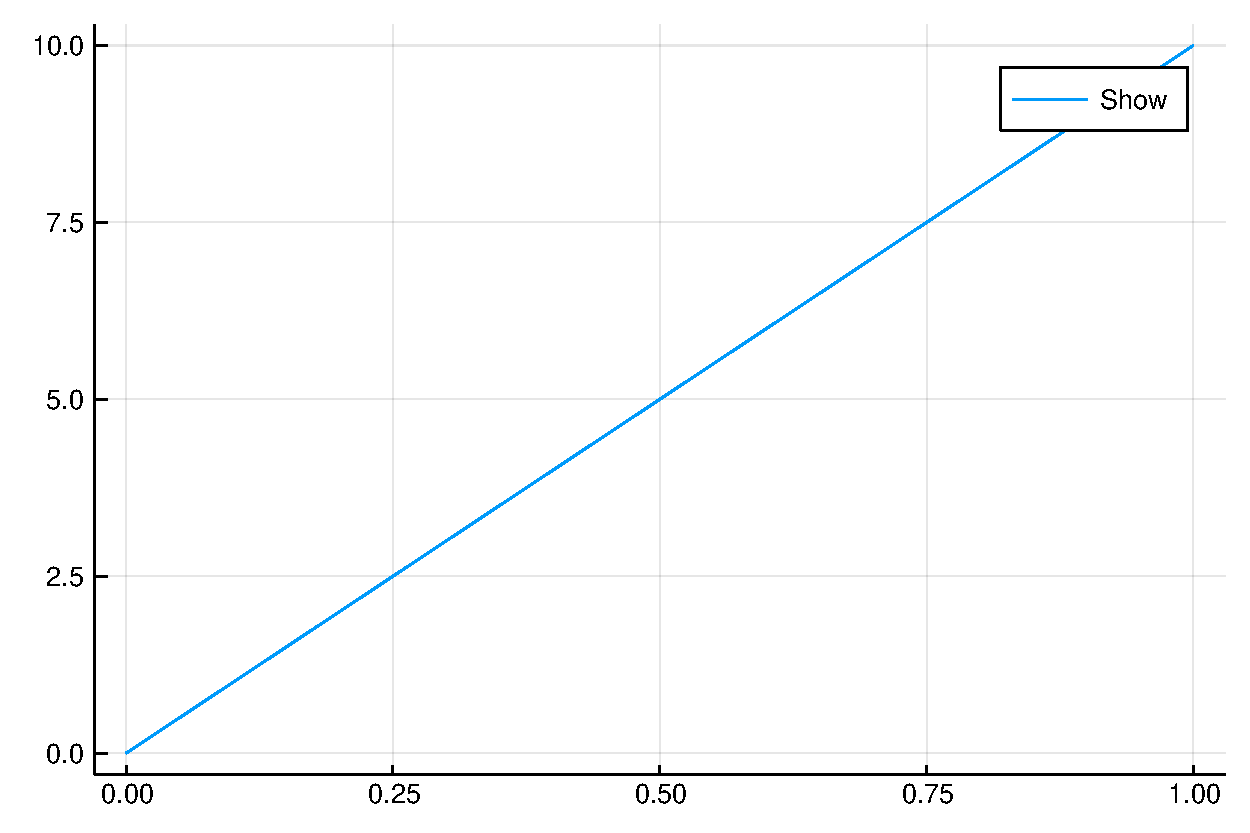
\includegraphics[width=\linewidth]{figures/A1_1_1.pdf}
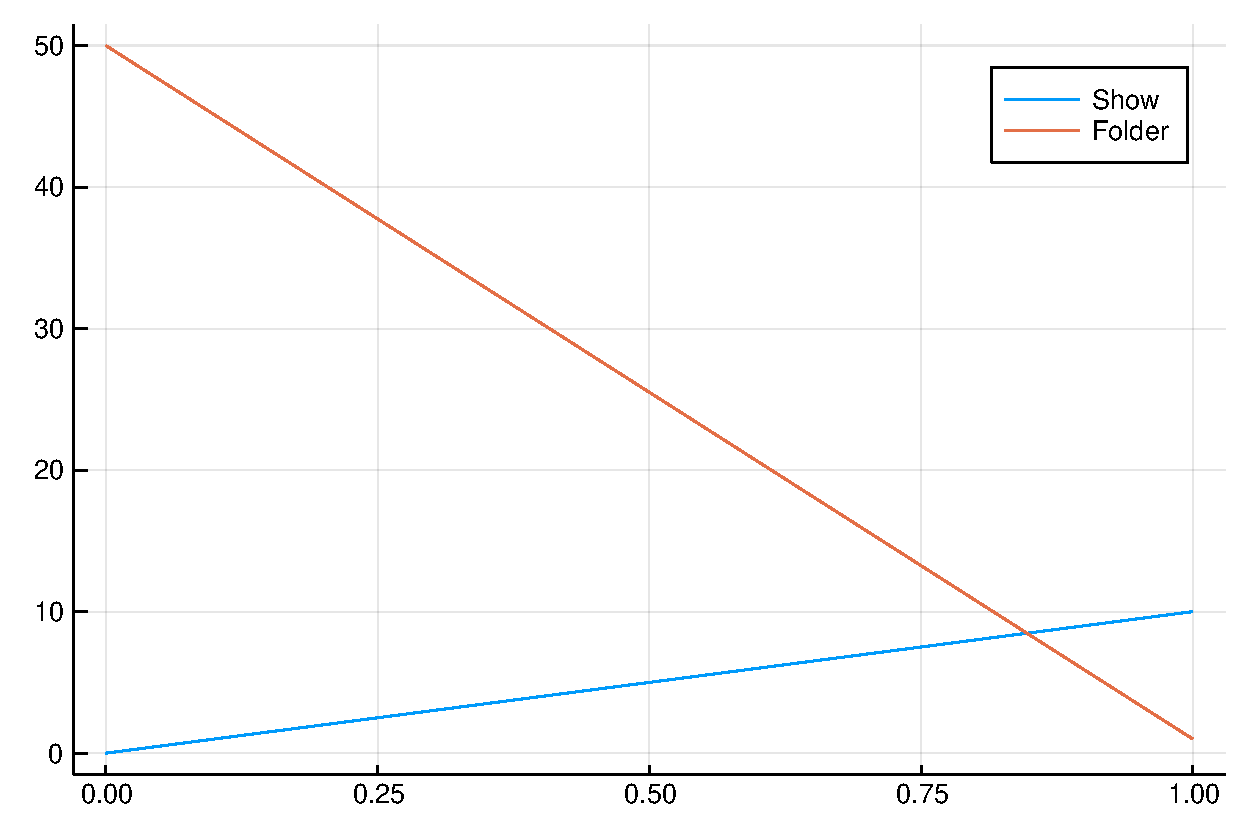
\includegraphics[width=\linewidth]{figures/A1_1_2.pdf}
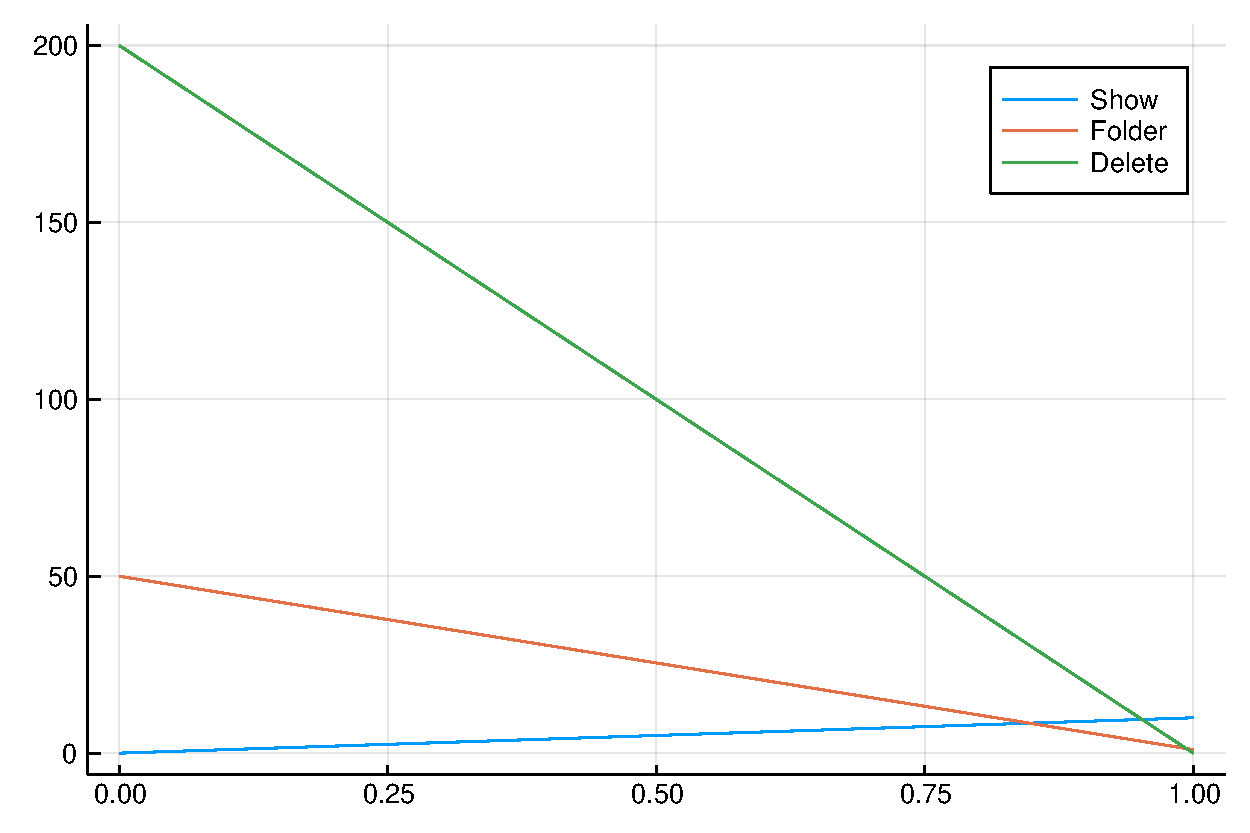
\includegraphics[width=\linewidth]{figures/A1_1_3.pdf}

\begin{itemize}
\item[2. ] [2pts] Write a function that computes the optimal action given the probability of spam.

\end{itemize}

\begin{lstlisting}
(*@\HLJLk{function}@*) (*@\HLJLnf{optimal{\_}action}@*)(*@\HLJLp{(}@*)(*@\HLJLn{prob{\_}spam}@*)(*@\HLJLp{)}@*)
  (*@\HLJLcs{{\#}TODO:}@*) (*@\HLJLcs{return}@*) (*@\HLJLcs{best}@*) (*@\HLJLcs{action}@*) (*@\HLJLcs{given}@*) (*@\HLJLcs{the}@*) (*@\HLJLcs{probability}@*) (*@\HLJLcs{of}@*) (*@\HLJLcs{spam.}@*)
  (*@\HLJLcs{{\#}}@*) (*@\HLJLcs{Hint:}@*) (*@\HLJLcs{Julia{\textquotesingle}s}@*) (*@\HLJLcs{findmin}@*) (*@\HLJLcs{function}@*) (*@\HLJLcs{might}@*) (*@\HLJLcs{be}@*) (*@\HLJLcs{helpful.}@*)
  (*@\HLJLk{return}@*) (*@\HLJLnf{findmin}@*)(*@\HLJLp{([}@*)(*@\HLJLnf{expected{\_}loss{\_}of{\_}action}@*)(*@\HLJLp{(}@*)(*@\HLJLn{prob{\_}spam}@*)(*@\HLJLp{,}@*) (*@\HLJLn{action}@*)(*@\HLJLp{)}@*) (*@\HLJLk{for}@*) (*@\HLJLn{action}@*) (*@\HLJLkp{in}@*) (*@\HLJLni{1}@*)(*@\HLJLoB{:}@*)(*@\HLJLn{num{\_}actions}@*)(*@\HLJLp{])[}@*)(*@\HLJLni{2}@*)(*@\HLJLp{]}@*)
(*@\HLJLk{end}@*)
(*@\HLJLk{using}@*) (*@\HLJLn{Test}@*)
(*@\HLJLnd{@testset}@*) (*@\HLJLs{"{}optimal{\_}action()}@*) (*@\HLJLs{correct"{}}@*) (*@\HLJLk{begin}@*)
  (*@\HLJLnd{@test}@*) (*@\HLJLnf{optimal{\_}action}@*)(*@\HLJLp{(}@*)(*@\HLJLnfB{0.5}@*)(*@\HLJLp{)}@*) (*@\HLJLoB{==}@*) (*@\HLJLni{1}@*)
  (*@\HLJLnd{@test}@*) (*@\HLJLnf{optimal{\_}action}@*)(*@\HLJLp{(}@*)(*@\HLJLni{1}@*)(*@\HLJLp{)}@*) (*@\HLJLoB{==}@*) (*@\HLJLni{3}@*)
  (*@\HLJLnd{@test}@*) (*@\HLJLnf{optimal{\_}action}@*)(*@\HLJLp{(}@*)(*@\HLJLni{0}@*)(*@\HLJLp{)}@*) (*@\HLJLoB{==}@*) (*@\HLJLni{1}@*)
(*@\HLJLk{end}@*)
\end{lstlisting}

\begin{lstlisting}
Test Summary:            | Pass  Total
optimal_action() correct |    3      3
Test.DefaultTestSet("optimal_action() correct", Any[], 3, false)
\end{lstlisting}


\begin{itemize}
\item[3. ] [4pts] Plot the expected loss of the optimal action as a function of the probability of spam.

\end{itemize}
Color the line according to the optimal action for that probability of spam.


\begin{lstlisting}
(*@\HLJLn{prob{\_}range}@*) (*@\HLJLoB{=}@*) (*@\HLJLnf{range}@*)(*@\HLJLp{(}@*)(*@\HLJLni{0}@*)(*@\HLJLp{,}@*) (*@\HLJLn{stop}@*)(*@\HLJLoB{=}@*)(*@\HLJLnfB{1.}@*)(*@\HLJLp{,}@*) (*@\HLJLn{length}@*)(*@\HLJLoB{=}@*)(*@\HLJLni{500}@*)(*@\HLJLp{)}@*)
  (*@\HLJLn{optimal{\_}losses}@*) (*@\HLJLoB{=}@*) (*@\HLJLp{[]}@*)
  (*@\HLJLn{optimal{\_}actions}@*) (*@\HLJLoB{=}@*) (*@\HLJLp{[]}@*)
  (*@\HLJLk{for}@*) (*@\HLJLn{p}@*) (*@\HLJLkp{in}@*) (*@\HLJLn{prob{\_}range}@*)
      (*@\HLJLcs{{\#}}@*) (*@\HLJLcs{TODO:}@*)  (*@\HLJLcs{Compute}@*) (*@\HLJLcs{the}@*) (*@\HLJLcs{optimal}@*) (*@\HLJLcs{action}@*) (*@\HLJLcs{and}@*) (*@\HLJLcs{its}@*) (*@\HLJLcs{expected}@*) (*@\HLJLcs{loss}@*) (*@\HLJLcs{for}@*)
      (*@\HLJLcs{{\#}}@*) (*@\HLJLcs{probability}@*) (*@\HLJLcs{of}@*) (*@\HLJLcs{spam}@*) (*@\HLJLcs{given}@*) (*@\HLJLcs{by}@*) (*@\HLJLcs{p.}@*)
      (*@\HLJLn{opt}@*) (*@\HLJLoB{=}@*) (*@\HLJLnf{optimal{\_}action}@*)(*@\HLJLp{(}@*)(*@\HLJLn{p}@*)(*@\HLJLp{)}@*)
      (*@\HLJLnf{append!}@*)(*@\HLJLp{(}@*)(*@\HLJLn{optimal{\_}actions}@*)(*@\HLJLp{,}@*) (*@\HLJLn{opt}@*)(*@\HLJLp{)}@*)
      (*@\HLJLnf{append!}@*)(*@\HLJLp{(}@*)(*@\HLJLn{optimal{\_}losses}@*)(*@\HLJLp{,}@*) (*@\HLJLnf{expected{\_}loss{\_}of{\_}action}@*)(*@\HLJLp{(}@*)(*@\HLJLn{p}@*)(*@\HLJLp{,}@*) (*@\HLJLn{opt}@*)(*@\HLJLp{))}@*)
  (*@\HLJLk{end}@*)

  (*@\HLJLnf{plot}@*)(*@\HLJLp{(}@*)(*@\HLJLn{prob{\_}range}@*)(*@\HLJLp{,}@*) (*@\HLJLn{optimal{\_}losses}@*)(*@\HLJLp{,}@*) (*@\HLJLn{linecolor}@*)(*@\HLJLoB{=}@*)(*@\HLJLn{optimal{\_}actions}@*)(*@\HLJLp{,}@*)
  (*@\HLJLn{label}@*) (*@\HLJLoB{=}@*) (*@\HLJLs{"{}expectedloss"{}}@*)(*@\HLJLp{)}@*)
  (*@\HLJLnf{savefig}@*)(*@\HLJLp{(}@*)(*@\HLJLs{"{}expectedlossToprob.pdf"{}}@*)(*@\HLJLp{)}@*)
\end{lstlisting}


\begin{itemize}
\item[4. ] [4pts] For exactly which range of the probabilities of an email being spam should we delete an email?

\end{itemize}
Find the exact answer by hand using algebra. $\\$ Given probability of spam $p\in [0,1]$, the expected loss of deleting, foldering and showing such email are respectively $10p,p+50(1-p),200(1-p)$. Making a decision of deletion is equivalent to expected loss of deletion being smaller than expected loss of the other two actions. We have: $200(1-p)\leq p+50(1-p)$ and $200(1-p) \leq 10p$, which implies $p \geq \frac{150}{151}$ and $p \geq \frac{20}{21}$. So when $\frac{150}{151} \leq p \leq 1$, we'll delete the mail.

\section{Regression}
\subsection{Manually Derived Linear Regression [10pts]}
Suppose that $X \in \mathbb{R}^{m \times n}$ with $n \geq m$ and $Y \in \mathbb{R}^n$, and that $Y \sim \mathcal{N}(X^T\beta, \sigma^2 I)$.

In this question you will derive the result that the maximum likelihood estimate $\hat\beta$ of $\beta$ is given by

\[
\hat\beta = (XX^T)^{-1}XY
\]
\begin{itemize}
\item[1. ] [1pts] What happens if $n < m$?

\end{itemize}
We'll have more variables than observations which will cause overfitting.

\begin{itemize}
\item[2. ] [2pts] What are the expectation and covariance matrix of $\hat\beta$, for a given true value of $\beta$?

\end{itemize}
\[
E(\hat{\beta}) = E((XX^{T})^{-1}XY) = (XX^{T})^{-1}XE(Y) = (XX^{T})^{-1}XX^{T}\beta
= I\beta = \beta
\]
\begin{itemize}
\item[3. ] [2pts] Show that maximizing the likelihood is equivalent to minimizing the squared error $\sum_{i=1}^n (y_i - x_i\beta)^2$. [Hint: Use $\sum_{i=1}^n a_i^2 = a^Ta$]

\end{itemize}
Since $Y\sim N(X^{T}\beta, \sigma^2I)$, we have:

\[
L(\beta) = f(Y|X,\beta) =
\frac{1}{(2\pi)^{n/2}|\sigma^2I|^{1/2}}exp(-1/2(Y-X^T\beta)^T(\sigma^2I)^{-1}(Y-X^T\beta))
\]
Since exponential function is increasing, maximizing the likelihood function is equivalent to minimizing $(Y-X^T\beta)^T(Y-X^T\beta)=\sum_{i=1}^n(y_i-x_i\beta)^2$ with respect to $\beta$, where $x_i$ is the $i^{th}$ column of $X$.

\begin{itemize}
\item[4. ] [2pts] Write the squared error in vector notation, (see above hint), expand the expression, and collect like terms. [Hint: Use $\beta^Tx^Ty = y^Tx\beta$ and $x^Tx$ is symmetric]

\end{itemize}

\begin{align}
\sum_{i=1}^n(y_i-x_i\beta)^2
&=(Y-X^T\beta)^T(Y-X^T\beta) \\
&=(Y^T-\beta^TX)(Y-X^T\beta)\\
&=Y^TY-\beta^TXY-Y^TX^T\beta+\beta^TX^TX\beta \\
&=Y^TY-2Y^TX^T\beta+\beta^TX^TX\beta\hspace{15mm}\text{because $Y^TX^T\beta$ is symmetric}
\end{align}
\begin{itemize}
\item[5. ] [3pts] Use the likelihood expression to write the negative log-likelihood.  Write the derivative of the negative log-likelihood with respect to $\beta$, set equal to zero, and solve to show the maximum likelihood estimate $\hat\beta$ as above.

\end{itemize}
\[
L(\beta) = f(Y|X,\beta) =
\frac{1}{(2\pi)^{n/2}|\sigma^2I|^{1/2}}exp(-1/(2\sigma^2)I(Y^TY-2\beta^TXY+\beta^TX^TX\beta))
\]
We have:


\begin{align}
l(\beta) &= -log(L(\beta))\\
& = -log(\frac{1}{(2\pi)^{n/2}|\sigma^2I|^{1/2}})
-1/(2\sigma^2)I(Y^TY-2\beta^TXY+\beta^TX^TX\beta))\\
l'(\beta)&= -1/(2\sigma^2)(0-2XY+(XX^T+(XX^T)^T)\beta)\\
&=-1/(2\sigma^2)(-2XY+2XX^T\beta)\\
&=0\\
&2XX^T\beta=2XY\\
&\hat{\beta} = (XX^T)^{-1}XY
\end{align}
And $l''(\beta) = -1/(2\sigma^2)(2X^TX) < 0$ so $\hat{\beta}$ indeed is a maximum.

\subsection{Toy Data [2pts]}
For visualization purposes and to minimize computational resources we will work with 1-dimensional toy data.

That is $X \in \mathbb{R}^{m \times n}$ where $m=1$.

We will learn models for 3 target functions

\begin{itemize}
\item \texttt{target\_f1}, linear trend with constant noise.


\item \texttt{target\_f2}, linear trend with heteroskedastic noise.


\item \texttt{target\_f3}, non-linear trend with heteroskedastic noise.

\end{itemize}

\begin{lstlisting}
(*@\HLJLk{using}@*) (*@\HLJLn{LinearAlgebra}@*)

(*@\HLJLk{function}@*) (*@\HLJLnf{target{\_}f1}@*)(*@\HLJLp{(}@*)(*@\HLJLn{x}@*)(*@\HLJLp{,}@*) (*@\HLJLn{\ensuremath{\sigma}{\_}true}@*)(*@\HLJLoB{=}@*)(*@\HLJLnfB{0.3}@*)(*@\HLJLp{)}@*)
  (*@\HLJLn{noise}@*) (*@\HLJLoB{=}@*) (*@\HLJLnf{randn}@*)(*@\HLJLp{(}@*)(*@\HLJLnf{size}@*)(*@\HLJLp{(}@*)(*@\HLJLn{x}@*)(*@\HLJLp{))}@*)
  (*@\HLJLn{y}@*) (*@\HLJLoB{=}@*) (*@\HLJLni{2}@*)(*@\HLJLn{x}@*) (*@\HLJLoB{.+}@*) (*@\HLJLn{\ensuremath{\sigma}{\_}true}@*)(*@\HLJLoB{.*}@*)(*@\HLJLn{noise}@*)
  (*@\HLJLk{return}@*) (*@\HLJLnf{vec}@*)(*@\HLJLp{(}@*)(*@\HLJLn{y}@*)(*@\HLJLp{)}@*)
(*@\HLJLk{end}@*)

(*@\HLJLk{function}@*) (*@\HLJLnf{target{\_}f2}@*)(*@\HLJLp{(}@*)(*@\HLJLn{x}@*)(*@\HLJLp{)}@*)
  (*@\HLJLn{noise}@*) (*@\HLJLoB{=}@*) (*@\HLJLnf{randn}@*)(*@\HLJLp{(}@*)(*@\HLJLnf{size}@*)(*@\HLJLp{(}@*)(*@\HLJLn{x}@*)(*@\HLJLp{))}@*)
  (*@\HLJLn{y}@*) (*@\HLJLoB{=}@*) (*@\HLJLni{2}@*)(*@\HLJLn{x}@*) (*@\HLJLoB{+}@*) (*@\HLJLn{norm}@*)(*@\HLJLoB{.}@*)(*@\HLJLp{(}@*)(*@\HLJLn{x}@*)(*@\HLJLp{)}@*)(*@\HLJLoB{*}@*)(*@\HLJLnfB{0.3}@*)(*@\HLJLoB{.*}@*)(*@\HLJLn{noise}@*)
  (*@\HLJLk{return}@*) (*@\HLJLnf{vec}@*)(*@\HLJLp{(}@*)(*@\HLJLn{y}@*)(*@\HLJLp{)}@*)
(*@\HLJLk{end}@*)

(*@\HLJLk{function}@*) (*@\HLJLnf{target{\_}f3}@*)(*@\HLJLp{(}@*)(*@\HLJLn{x}@*)(*@\HLJLp{)}@*)
  (*@\HLJLn{noise}@*) (*@\HLJLoB{=}@*) (*@\HLJLnf{randn}@*)(*@\HLJLp{(}@*)(*@\HLJLnf{size}@*)(*@\HLJLp{(}@*)(*@\HLJLn{x}@*)(*@\HLJLp{))}@*)
  (*@\HLJLn{y}@*) (*@\HLJLoB{=}@*) (*@\HLJLni{2}@*)(*@\HLJLn{x}@*) (*@\HLJLoB{+}@*) (*@\HLJLni{5}@*)(*@\HLJLn{sin}@*)(*@\HLJLoB{.}@*)(*@\HLJLp{(}@*)(*@\HLJLnfB{0.5}@*)(*@\HLJLoB{*}@*)(*@\HLJLn{x}@*)(*@\HLJLp{)}@*) (*@\HLJLoB{+}@*) (*@\HLJLn{norm}@*)(*@\HLJLoB{.}@*)(*@\HLJLp{(}@*)(*@\HLJLn{x}@*)(*@\HLJLp{)}@*)(*@\HLJLoB{*}@*)(*@\HLJLnfB{0.3}@*)(*@\HLJLoB{.*}@*)(*@\HLJLn{noise}@*)
  (*@\HLJLk{return}@*) (*@\HLJLnf{vec}@*)(*@\HLJLp{(}@*)(*@\HLJLn{y}@*)(*@\HLJLp{)}@*)
(*@\HLJLk{end}@*)
\end{lstlisting}

\begin{lstlisting}
target_f3 (generic function with 1 method)
\end{lstlisting}


\begin{itemize}
\item[1. ] [1pts] Write a function which produces a batch of data $x \sim \text{Uniform}(0,20)$ and \texttt{y = target\_f(x)}

\end{itemize}

\begin{lstlisting}
(*@\HLJLk{function}@*) (*@\HLJLnf{sample{\_}batch}@*)(*@\HLJLp{(}@*)(*@\HLJLn{target{\_}f}@*)(*@\HLJLp{,}@*) (*@\HLJLn{batch{\_}size}@*)(*@\HLJLp{)}@*)
  (*@\HLJLn{x}@*) (*@\HLJLoB{=}@*) (*@\HLJLp{(}@*)(*@\HLJLni{20}@*)(*@\HLJLoB{*}@*)(*@\HLJLnf{rand}@*)(*@\HLJLp{(}@*)(*@\HLJLn{batch{\_}size}@*)(*@\HLJLp{))}@*)(*@\HLJLoB{{\textquotesingle}}@*)
  (*@\HLJLn{y}@*) (*@\HLJLoB{=}@*) (*@\HLJLnf{target{\_}f}@*)(*@\HLJLp{(}@*)(*@\HLJLn{x}@*)(*@\HLJLp{)}@*)
  (*@\HLJLk{return}@*) (*@\HLJLp{(}@*)(*@\HLJLn{x}@*)(*@\HLJLp{,}@*)(*@\HLJLn{y}@*)(*@\HLJLp{)}@*)
(*@\HLJLk{end}@*)
\end{lstlisting}

\begin{lstlisting}
sample_batch (generic function with 1 method)
\end{lstlisting}


\begin{lstlisting}
(*@\HLJLk{using}@*) (*@\HLJLn{Test}@*)
(*@\HLJLnd{@testset}@*) (*@\HLJLs{"{}sample}@*) (*@\HLJLs{dimensions}@*) (*@\HLJLs{are}@*) (*@\HLJLs{correct"{}}@*) (*@\HLJLk{begin}@*)
  (*@\HLJLn{m}@*) (*@\HLJLoB{=}@*) (*@\HLJLni{1}@*) (*@\HLJLcs{{\#}}@*) (*@\HLJLcs{dimensionality}@*)
  (*@\HLJLn{n}@*) (*@\HLJLoB{=}@*) (*@\HLJLni{200}@*) (*@\HLJLcs{{\#}}@*) (*@\HLJLcs{batch-size}@*)
  (*@\HLJLk{for}@*) (*@\HLJLn{target{\_}f}@*) (*@\HLJLkp{in}@*) (*@\HLJLp{(}@*)(*@\HLJLn{target{\_}f1}@*)(*@\HLJLp{,}@*) (*@\HLJLn{target{\_}f2}@*)(*@\HLJLp{,}@*) (*@\HLJLn{target{\_}f3}@*)(*@\HLJLp{)}@*)
    (*@\HLJLn{x}@*)(*@\HLJLp{,}@*)(*@\HLJLn{y}@*) (*@\HLJLoB{=}@*) (*@\HLJLnf{sample{\_}batch}@*)(*@\HLJLp{(}@*)(*@\HLJLn{target{\_}f}@*)(*@\HLJLp{,}@*)(*@\HLJLn{n}@*)(*@\HLJLp{)}@*)
    (*@\HLJLnd{@test}@*) (*@\HLJLnf{size}@*)(*@\HLJLp{(}@*)(*@\HLJLn{x}@*)(*@\HLJLp{)}@*) (*@\HLJLoB{==}@*) (*@\HLJLp{(}@*)(*@\HLJLn{m}@*)(*@\HLJLp{,}@*)(*@\HLJLn{n}@*)(*@\HLJLp{)}@*)
    (*@\HLJLnd{@test}@*) (*@\HLJLnf{size}@*)(*@\HLJLp{(}@*)(*@\HLJLn{y}@*)(*@\HLJLp{)}@*) (*@\HLJLoB{==}@*) (*@\HLJLp{(}@*)(*@\HLJLn{n}@*)(*@\HLJLp{,)}@*)
  (*@\HLJLk{end}@*)
(*@\HLJLk{end}@*)
\end{lstlisting}

\begin{lstlisting}
Test Summary:                 | Pass  Total
sample dimensions are correct |    6      6
Test.DefaultTestSet("sample dimensions are correct", Any[], 6, false)
\end{lstlisting}


\begin{itemize}
\item[2. ] [1pts] For all three targets, plot a $n=1000$ sample of the data.  \textbf{Note: You will use these plots later, in your writeup display once other questions are complete.}

\end{itemize}

\begin{lstlisting}
(*@\HLJLk{using}@*) (*@\HLJLn{Plots}@*)
(*@\HLJLn{n}@*) (*@\HLJLoB{=}@*) (*@\HLJLni{1000}@*)
(*@\HLJLn{x1}@*)(*@\HLJLp{,}@*)(*@\HLJLn{y1}@*) (*@\HLJLoB{=}@*) (*@\HLJLnf{sample{\_}batch}@*)(*@\HLJLp{(}@*)(*@\HLJLn{target{\_}f1}@*)(*@\HLJLp{,}@*)(*@\HLJLn{n}@*)(*@\HLJLp{)}@*)
(*@\HLJLn{plot{\_}f1}@*) (*@\HLJLoB{=}@*) (*@\HLJLnf{plot}@*)(*@\HLJLp{(}@*)(*@\HLJLn{x1}@*)(*@\HLJLoB{{\textquotesingle}}@*)(*@\HLJLp{,}@*) (*@\HLJLn{y1}@*)(*@\HLJLp{)}@*)

(*@\HLJLn{x2}@*)(*@\HLJLp{,}@*)(*@\HLJLn{y2}@*) (*@\HLJLoB{=}@*) (*@\HLJLnf{sample{\_}batch}@*)(*@\HLJLp{(}@*)(*@\HLJLn{target{\_}f2}@*)(*@\HLJLp{,}@*)(*@\HLJLn{n}@*)(*@\HLJLp{)}@*)
(*@\HLJLn{plot{\_}f2}@*) (*@\HLJLoB{=}@*) (*@\HLJLnf{plot}@*)(*@\HLJLp{(}@*)(*@\HLJLn{x2}@*)(*@\HLJLoB{{\textquotesingle}}@*)(*@\HLJLp{,}@*) (*@\HLJLn{y2}@*)(*@\HLJLp{)}@*)

(*@\HLJLn{x3}@*)(*@\HLJLp{,}@*)(*@\HLJLn{y3}@*) (*@\HLJLoB{=}@*) (*@\HLJLnf{sample{\_}batch}@*)(*@\HLJLp{(}@*)(*@\HLJLn{target{\_}f3}@*)(*@\HLJLp{,}@*)(*@\HLJLn{n}@*)(*@\HLJLp{)}@*)
(*@\HLJLn{plot{\_}f3}@*) (*@\HLJLoB{=}@*) (*@\HLJLnf{plot}@*)(*@\HLJLp{(}@*)(*@\HLJLn{x3}@*)(*@\HLJLoB{{\textquotesingle}}@*)(*@\HLJLp{,}@*) (*@\HLJLn{y3}@*)(*@\HLJLp{)}@*)
\end{lstlisting}

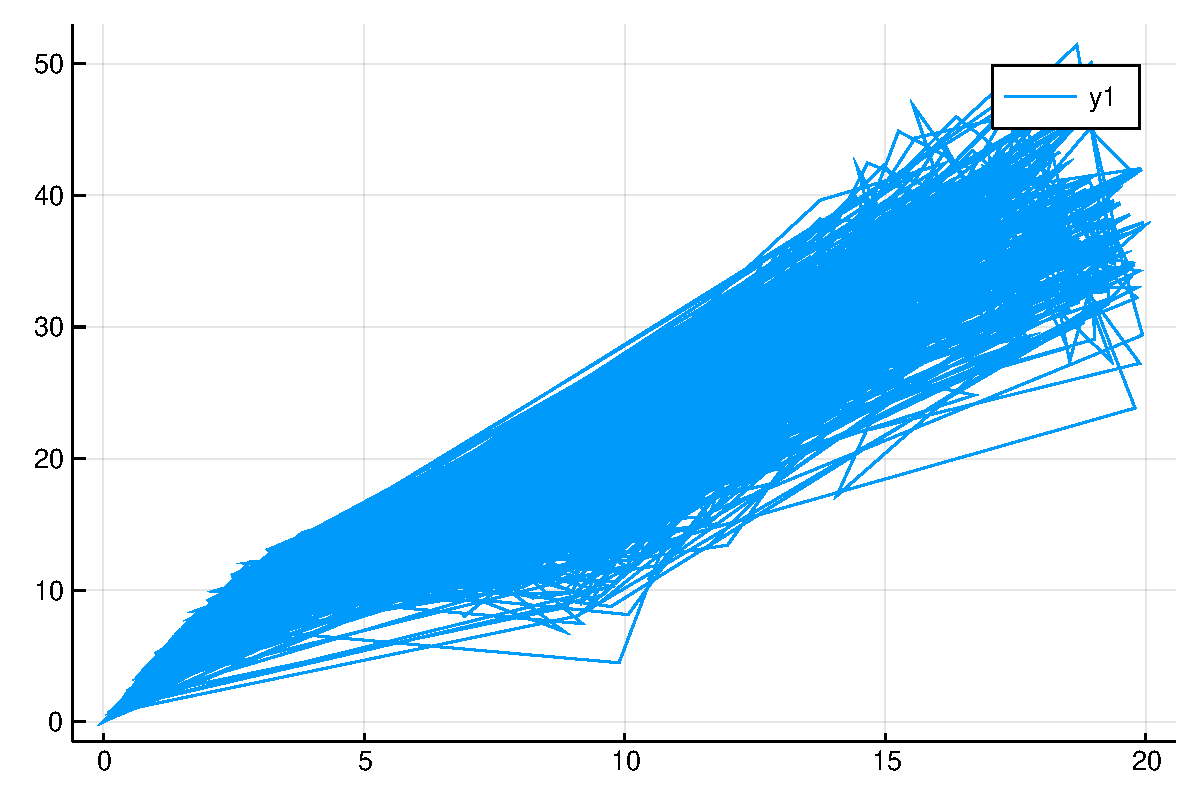
\includegraphics[width=\linewidth]{figures/A1_7_1.pdf}

\subsection{Linear Regression Model with $\hat \beta$ MLE [4pts]}
\begin{itemize}
\item[1. ] [2pts] Program the function that computes the the maximum likelihood estimate given $X$ and $Y$.  Use it to compute the estimate $\hat \beta$ for a $n=1000$ sample from each target function.

\end{itemize}

\begin{lstlisting}
(*@\HLJLk{function}@*) (*@\HLJLnf{beta{\_}mle}@*)(*@\HLJLp{(}@*)(*@\HLJLn{X}@*)(*@\HLJLp{,}@*)(*@\HLJLn{Y}@*)(*@\HLJLp{)}@*)
      (*@\HLJLn{beta}@*) (*@\HLJLoB{=}@*) (*@\HLJLnf{inv}@*)(*@\HLJLp{(}@*)(*@\HLJLn{X}@*)(*@\HLJLoB{*}@*)(*@\HLJLn{X}@*)(*@\HLJLoB{{\textquotesingle}}@*)(*@\HLJLp{)}@*)(*@\HLJLoB{*}@*)(*@\HLJLn{X}@*)(*@\HLJLoB{*}@*)(*@\HLJLn{Y}@*)
      (*@\HLJLk{return}@*) (*@\HLJLn{beta}@*)
    (*@\HLJLk{end}@*)

    (*@\HLJLk{using}@*) (*@\HLJLn{Test}@*)
    (*@\HLJLnd{@testset}@*) (*@\HLJLs{"{}beta{\_}mle}@*) (*@\HLJLs{computes}@*) (*@\HLJLs{correctly"{}}@*) (*@\HLJLk{begin}@*)
        (*@\HLJLn{X}@*) (*@\HLJLoB{=}@*) (*@\HLJLp{[}@*)(*@\HLJLni{3}@*) (*@\HLJLni{4}@*)(*@\HLJLp{]}@*)
        (*@\HLJLn{Y}@*) (*@\HLJLoB{=}@*) (*@\HLJLp{[}@*)(*@\HLJLni{1}@*)(*@\HLJLp{,}@*) (*@\HLJLni{2}@*)(*@\HLJLp{]}@*)
        (*@\HLJLnd{@test}@*) (*@\HLJLnf{beta{\_}mle}@*)(*@\HLJLp{(}@*)(*@\HLJLn{X}@*)(*@\HLJLp{,}@*)(*@\HLJLn{Y}@*)(*@\HLJLp{)}@*) (*@\HLJLoB{==}@*) (*@\HLJLp{[}@*)(*@\HLJLni{11}@*)(*@\HLJLoB{/}@*)(*@\HLJLni{25}@*)(*@\HLJLp{]}@*)
    (*@\HLJLk{end}@*)
\end{lstlisting}

\begin{lstlisting}
Test Summary:               | Pass  Total
beta_mle computes correctly |    1      1
\end{lstlisting}


\begin{lstlisting}
(*@\HLJLn{n}@*)(*@\HLJLoB{=}@*)(*@\HLJLni{1000}@*) (*@\HLJLcs{{\#}}@*) (*@\HLJLcs{batch{\_}size}@*)

    (*@\HLJLn{x{\_}1}@*)(*@\HLJLp{,}@*) (*@\HLJLn{y{\_}1}@*) (*@\HLJLoB{=}@*) (*@\HLJLnf{sample{\_}batch}@*)(*@\HLJLp{(}@*)(*@\HLJLn{target{\_}f1}@*)(*@\HLJLp{,}@*)(*@\HLJLn{n}@*)(*@\HLJLp{)}@*)
    (*@\HLJLn{\ensuremath{\beta}{\_}mle{\_}1}@*) (*@\HLJLoB{=}@*) (*@\HLJLnf{beta{\_}mle}@*)(*@\HLJLp{(}@*)(*@\HLJLn{x{\_}1}@*)(*@\HLJLp{,}@*)(*@\HLJLn{y{\_}1}@*)(*@\HLJLp{)}@*)

    (*@\HLJLn{x{\_}2}@*)(*@\HLJLp{,}@*) (*@\HLJLn{y{\_}2}@*) (*@\HLJLoB{=}@*) (*@\HLJLnf{sample{\_}batch}@*)(*@\HLJLp{(}@*)(*@\HLJLn{target{\_}f2}@*)(*@\HLJLp{,}@*)(*@\HLJLn{n}@*)(*@\HLJLp{)}@*)
    (*@\HLJLn{\ensuremath{\beta}{\_}mle{\_}2}@*) (*@\HLJLoB{=}@*) (*@\HLJLnf{beta{\_}mle}@*)(*@\HLJLp{(}@*)(*@\HLJLn{x{\_}2}@*)(*@\HLJLp{,}@*)(*@\HLJLn{y{\_}2}@*)(*@\HLJLp{)}@*)

    (*@\HLJLn{x{\_}3}@*)(*@\HLJLp{,}@*) (*@\HLJLn{y{\_}3}@*) (*@\HLJLoB{=}@*) (*@\HLJLnf{sample{\_}batch}@*)(*@\HLJLp{(}@*)(*@\HLJLn{target{\_}f2}@*)(*@\HLJLp{,}@*)(*@\HLJLn{n}@*)(*@\HLJLp{)}@*)
    (*@\HLJLn{\ensuremath{\beta}{\_}mle{\_}3}@*) (*@\HLJLoB{=}@*) (*@\HLJLnf{sample{\_}batch}@*)(*@\HLJLp{(}@*)(*@\HLJLn{target{\_}f3}@*)(*@\HLJLp{,}@*)(*@\HLJLn{n}@*)(*@\HLJLp{)}@*)
\end{lstlisting}

\begin{lstlisting}
([1.0886936683176884 12.038451315332491 (*@\ensuremath{\dots}@*) 10.909389875725225 1.292896498556
0398], [5.493507091508028, 26.256122848944877, 36.08458242728992, 7.1836498
373402895, 21.460978370892413, 27.5723550808766, 24.52465402078307, 16.1458
19300176917, 8.349165248437437, 22.059783341354386  (*@\ensuremath{\dots}@*)  13.800274324722649, 
1.9544285555808767, 15.440576241347216, 31.66671690732593, 35.6353229812438
7, 9.882316870977519, 27.8981649286618, 14.305563125879091, 16.042001989940
81, 5.032675714978786])
\end{lstlisting}


\begin{itemize}
\item[2. ] [2pts] For each function, plot the linear regression model given by $Y \sim \mathcal{N}(X^T\hat\beta, \sigma^2 I)$ for $\sigma=1.$.  This plot should have the line of best fit given by the maximum likelihood estimate, as well as a shaded region around the line corresponding to plus/minus one standard deviation (i.e. the fixed uncertainty $\sigma=1.0$).  Using \texttt{Plots.jl} this shaded uncertainty region can be achieved with the \texttt{ribbon} keyword argument.  \textbf{Display 3 plots, one for each target function, showing samples of data and maximum likelihood estimate linear regression model}

\end{itemize}

\begin{lstlisting}
(*@\HLJLnf{sort!}@*)(*@\HLJLp{(}@*)(*@\HLJLn{x{\_}1}@*)(*@\HLJLoB{{\textquotesingle}}@*)(*@\HLJLp{)}@*)
(*@\HLJLnf{plot!}@*)(*@\HLJLp{(}@*)(*@\HLJLn{plot{\_}f1}@*)(*@\HLJLp{,}@*) (*@\HLJLn{x{\_}1}@*)(*@\HLJLoB{{\textquotesingle}}@*)(*@\HLJLp{,}@*) (*@\HLJLp{(}@*)(*@\HLJLn{x{\_}1}@*)(*@\HLJLp{)}@*)(*@\HLJLoB{{\textquotesingle}*}@*)(*@\HLJLn{\ensuremath{\beta}{\_}mle{\_}1}@*)(*@\HLJLp{,}@*)(*@\HLJLn{color}@*) (*@\HLJLoB{=}@*) (*@\HLJLs{"{}red"{}}@*)(*@\HLJLp{,}@*)(*@\HLJLn{ribbon}@*) (*@\HLJLoB{=}@*) (*@\HLJLni{1}@*)(*@\HLJLp{)}@*)
\end{lstlisting}

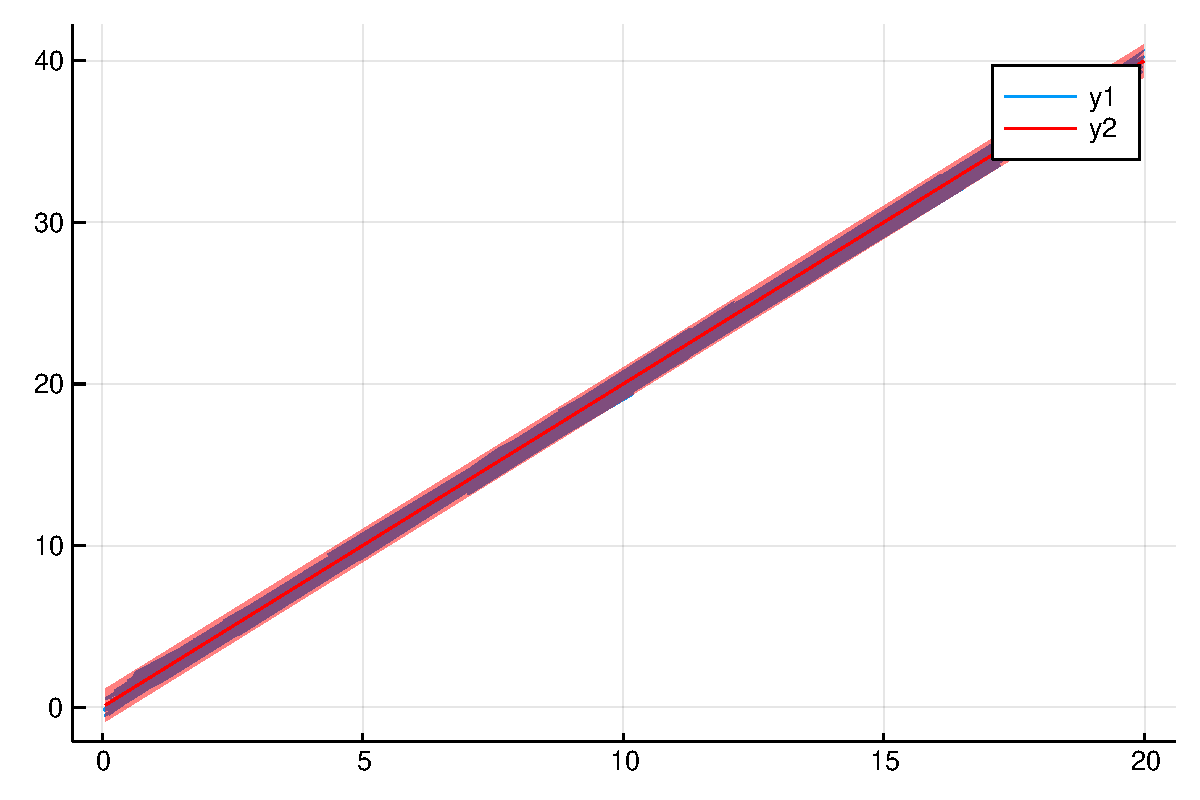
\includegraphics[width=\linewidth]{figures/A1_9_1.pdf}

\begin{lstlisting}
(*@\HLJLnf{sort!}@*)(*@\HLJLp{(}@*)(*@\HLJLn{x2}@*)(*@\HLJLoB{{\textquotesingle}}@*)(*@\HLJLp{)}@*)
(*@\HLJLnf{plot!}@*)(*@\HLJLp{(}@*)(*@\HLJLn{plot{\_}f2}@*)(*@\HLJLp{,}@*) (*@\HLJLn{x2}@*)(*@\HLJLoB{{\textquotesingle}}@*)(*@\HLJLp{,}@*) (*@\HLJLp{(}@*)(*@\HLJLn{x2}@*)(*@\HLJLp{)}@*)(*@\HLJLoB{{\textquotesingle}*}@*)(*@\HLJLn{\ensuremath{\beta}{\_}mle{\_}1}@*)(*@\HLJLp{,}@*)(*@\HLJLn{color}@*) (*@\HLJLoB{=}@*) (*@\HLJLs{"{}red"{}}@*)(*@\HLJLp{,}@*)(*@\HLJLn{ribbon}@*) (*@\HLJLoB{=}@*) (*@\HLJLni{1}@*)(*@\HLJLp{)}@*)
\end{lstlisting}

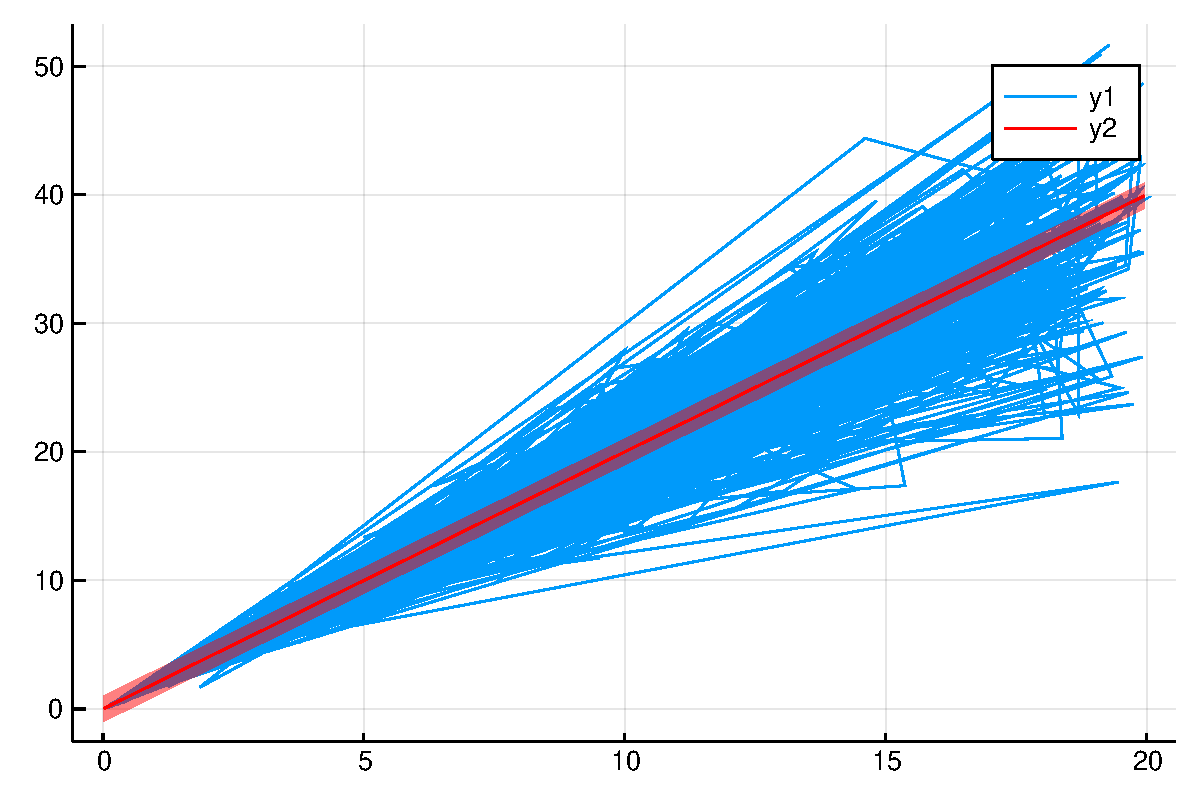
\includegraphics[width=\linewidth]{figures/A1_10_1.pdf}

\begin{lstlisting}
(*@\HLJLnf{sort!}@*)(*@\HLJLp{(}@*)(*@\HLJLn{x3}@*)(*@\HLJLoB{{\textquotesingle}}@*)(*@\HLJLp{)}@*)
(*@\HLJLnf{plot!}@*)(*@\HLJLp{(}@*)(*@\HLJLn{plot{\_}f3}@*)(*@\HLJLp{,}@*) (*@\HLJLp{(}@*)(*@\HLJLn{x3}@*)(*@\HLJLp{)}@*)(*@\HLJLoB{{\textquotesingle}}@*)(*@\HLJLp{,}@*) (*@\HLJLp{(}@*)(*@\HLJLn{x3}@*)(*@\HLJLp{)}@*)(*@\HLJLoB{{\textquotesingle}*}@*)(*@\HLJLn{\ensuremath{\beta}{\_}mle{\_}1}@*) (*@\HLJLp{,}@*)(*@\HLJLn{color}@*) (*@\HLJLoB{=}@*) (*@\HLJLs{"{}red"{}}@*)(*@\HLJLp{,}@*) (*@\HLJLn{ribbon}@*) (*@\HLJLoB{=}@*) (*@\HLJLni{1}@*)(*@\HLJLp{)}@*)
\end{lstlisting}

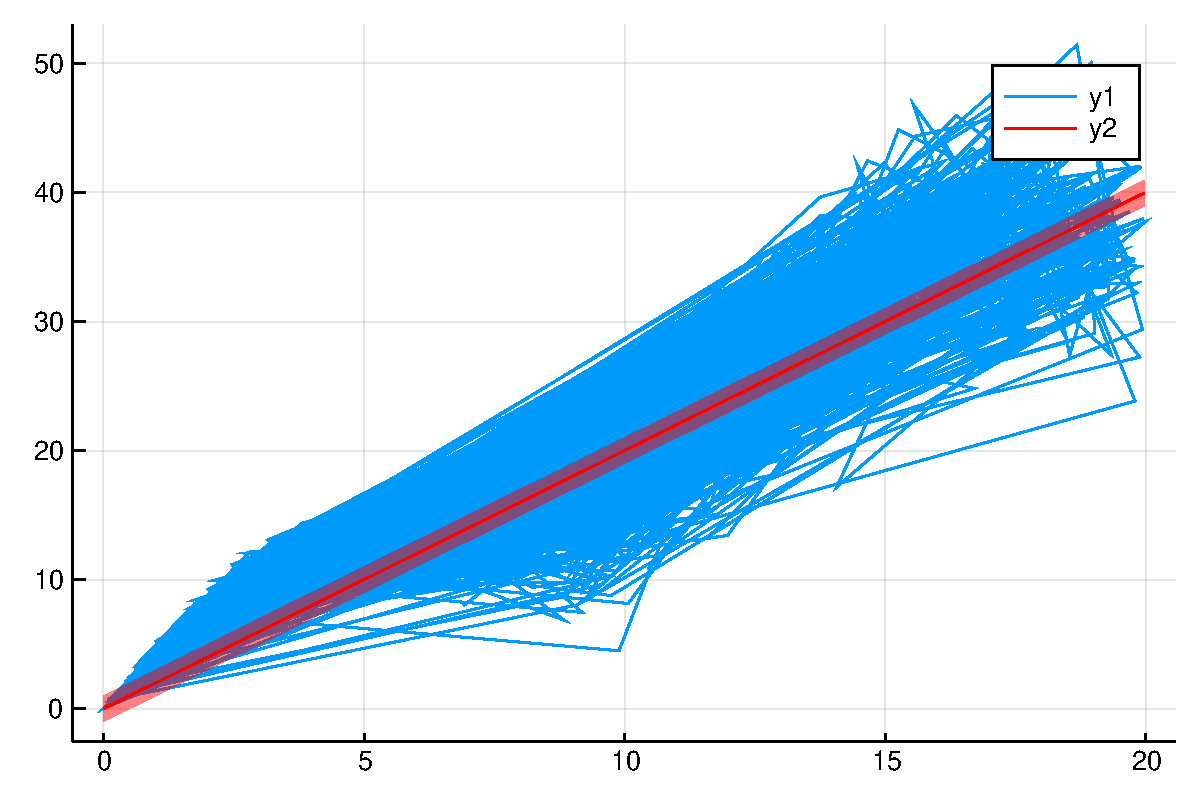
\includegraphics[width=\linewidth]{figures/A1_11_1.pdf}

\subsection{Log-likelihood of Data Under Model [6pts]}
\begin{itemize}
\item[1. ] [2pts] Write code for the function that computes the likelihood of $x$ under the Gaussian distribution $\mathcal{N}(\ensuremath{\mu},\ensuremath{\sigma})$.  For reasons that will be clear later, this function should be able to broadcast to the case where $x, \mu, \sigma$ are all vector valued  and return a vector of likelihoods with equivalent length, i.e., $x_i \sim \mathcal{N}(\mu_i,\sigma_i)$.

\end{itemize}

\begin{lstlisting}
(*@\HLJLk{function}@*) (*@\HLJLnf{gaussian{\_}log{\_}likelihood}@*)(*@\HLJLp{(}@*)(*@\HLJLn{\ensuremath{\mu}}@*)(*@\HLJLp{,}@*) (*@\HLJLn{\ensuremath{\sigma}}@*)(*@\HLJLp{,}@*) (*@\HLJLn{x}@*)(*@\HLJLp{)}@*)
  (*@\HLJLs{"{}"{}"{}}@*)
  (*@\HLJLs{compute}@*) (*@\HLJLs{log-likelihood}@*) (*@\HLJLs{of}@*) (*@\HLJLs{x}@*) (*@\HLJLs{under}@*) (*@\HLJLs{N(\ensuremath{\mu},\ensuremath{\sigma})}@*)
  (*@\HLJLs{"{}"{}"{}}@*)
  (*@\HLJLn{n}@*) (*@\HLJLoB{=}@*) (*@\HLJLnf{length}@*)(*@\HLJLp{(}@*)(*@\HLJLn{x}@*)(*@\HLJLp{)}@*)
  (*@\HLJLk{return}@*) (*@\HLJLoB{-}@*)(*@\HLJLni{1}@*)(*@\HLJLoB{/}@*)(*@\HLJLni{2}@*)(*@\HLJLoB{*}@*)(*@\HLJLnf{log}@*)(*@\HLJLp{(}@*)(*@\HLJLni{2}@*)(*@\HLJLoB{*}@*)(*@\HLJLn{pi}@*)(*@\HLJLp{)}@*) (*@\HLJLoB{-}@*) (*@\HLJLnf{log}@*)(*@\HLJLp{(}@*)(*@\HLJLn{\ensuremath{\sigma}}@*)(*@\HLJLp{)}@*) (*@\HLJLoB{-}@*) (*@\HLJLni{1}@*)(*@\HLJLoB{/}@*)(*@\HLJLp{(}@*)(*@\HLJLni{2}@*)(*@\HLJLn{\ensuremath{\sigma}}@*)(*@\HLJLoB{{\textasciicircum}}@*)(*@\HLJLni{2}@*)(*@\HLJLp{)}@*)(*@\HLJLoB{*}@*)(*@\HLJLp{(}@*)(*@\HLJLn{x}@*)(*@\HLJLoB{-}@*)(*@\HLJLn{\ensuremath{\mu}}@*)(*@\HLJLp{)}@*)(*@\HLJLoB{{\textasciicircum}}@*)(*@\HLJLni{2}@*)
(*@\HLJLk{end}@*)
\end{lstlisting}

\begin{lstlisting}
gaussian_log_likelihood (generic function with 1 method)
\end{lstlisting}


\begin{lstlisting}
(*@\HLJLcs{{\#}}@*) (*@\HLJLcs{Test}@*) (*@\HLJLcs{Gaussian}@*) (*@\HLJLcs{likelihood}@*) (*@\HLJLcs{against}@*) (*@\HLJLcs{standard}@*) (*@\HLJLcs{implementation}@*)
(*@\HLJLnd{@testset}@*) (*@\HLJLs{"{}Gaussian}@*) (*@\HLJLs{log}@*) (*@\HLJLs{likelihood"{}}@*) (*@\HLJLk{begin}@*)
(*@\HLJLk{using}@*) (*@\HLJLn{Distributions}@*)(*@\HLJLoB{:}@*) (*@\HLJLn{pdf}@*)(*@\HLJLp{,}@*) (*@\HLJLn{Normal}@*)
(*@\HLJLcs{{\#}}@*) (*@\HLJLcs{Scalar}@*) (*@\HLJLcs{mean}@*) (*@\HLJLcs{and}@*) (*@\HLJLcs{variance}@*)
(*@\HLJLn{x}@*) (*@\HLJLoB{=}@*) (*@\HLJLnf{randn}@*)(*@\HLJLp{()}@*)
(*@\HLJLn{\ensuremath{\mu}}@*) (*@\HLJLoB{=}@*) (*@\HLJLnf{randn}@*)(*@\HLJLp{()}@*)
(*@\HLJLn{\ensuremath{\sigma}}@*) (*@\HLJLoB{=}@*) (*@\HLJLnf{rand}@*)(*@\HLJLp{()}@*)
(*@\HLJLnd{@test}@*) (*@\HLJLnf{size}@*)(*@\HLJLp{(}@*)(*@\HLJLnf{gaussian{\_}log{\_}likelihood}@*)(*@\HLJLp{(}@*)(*@\HLJLn{\ensuremath{\mu}}@*)(*@\HLJLp{,}@*)(*@\HLJLn{\ensuremath{\sigma}}@*)(*@\HLJLp{,}@*)(*@\HLJLn{x}@*)(*@\HLJLp{))}@*) (*@\HLJLoB{==}@*) (*@\HLJLp{()}@*) (*@\HLJLcs{{\#}}@*) (*@\HLJLcs{Scalar}@*) (*@\HLJLcs{log-likelihood}@*)
(*@\HLJLnd{@test}@*) (*@\HLJLn{gaussian{\_}log{\_}likelihood}@*)(*@\HLJLoB{.}@*)(*@\HLJLp{(}@*)(*@\HLJLn{\ensuremath{\mu}}@*)(*@\HLJLp{,}@*)(*@\HLJLn{\ensuremath{\sigma}}@*)(*@\HLJLp{,}@*)(*@\HLJLn{x}@*)(*@\HLJLp{)}@*) (*@\HLJLoB{\ensuremath{\approx}}@*) (*@\HLJLn{log}@*)(*@\HLJLoB{.}@*)(*@\HLJLp{(}@*)(*@\HLJLn{pdf}@*)(*@\HLJLoB{.}@*)(*@\HLJLp{(}@*)(*@\HLJLnf{Normal}@*)(*@\HLJLp{(}@*)(*@\HLJLn{\ensuremath{\mu}}@*)(*@\HLJLp{,}@*)(*@\HLJLn{\ensuremath{\sigma}}@*)(*@\HLJLp{),}@*)(*@\HLJLn{x}@*)(*@\HLJLp{))}@*) (*@\HLJLcs{{\#}}@*) (*@\HLJLcs{Correct}@*) (*@\HLJLcs{Value}@*)
(*@\HLJLcs{{\#}}@*) (*@\HLJLcs{Vector}@*) (*@\HLJLcs{valued}@*) (*@\HLJLcs{x}@*) (*@\HLJLcs{under}@*) (*@\HLJLcs{constant}@*) (*@\HLJLcs{mean}@*) (*@\HLJLcs{and}@*) (*@\HLJLcs{variance}@*)
(*@\HLJLn{x}@*) (*@\HLJLoB{=}@*) (*@\HLJLnf{randn}@*)(*@\HLJLp{(}@*)(*@\HLJLni{100}@*)(*@\HLJLp{)}@*)
(*@\HLJLn{\ensuremath{\mu}}@*) (*@\HLJLoB{=}@*) (*@\HLJLnf{randn}@*)(*@\HLJLp{()}@*)
(*@\HLJLn{\ensuremath{\sigma}}@*) (*@\HLJLoB{=}@*) (*@\HLJLnf{rand}@*)(*@\HLJLp{()}@*)
(*@\HLJLnd{@test}@*) (*@\HLJLnf{size}@*)(*@\HLJLp{(}@*)(*@\HLJLn{gaussian{\_}log{\_}likelihood}@*)(*@\HLJLoB{.}@*)(*@\HLJLp{(}@*)(*@\HLJLn{\ensuremath{\mu}}@*)(*@\HLJLp{,}@*)(*@\HLJLn{\ensuremath{\sigma}}@*)(*@\HLJLp{,}@*)(*@\HLJLn{x}@*)(*@\HLJLp{))}@*) (*@\HLJLoB{==}@*) (*@\HLJLp{(}@*)(*@\HLJLni{100}@*)(*@\HLJLp{,)}@*) (*@\HLJLcs{{\#}}@*) (*@\HLJLcs{Vector}@*) (*@\HLJLcs{of}@*) (*@\HLJLcs{log-likelihoods}@*)
(*@\HLJLnd{@test}@*) (*@\HLJLn{gaussian{\_}log{\_}likelihood}@*)(*@\HLJLoB{.}@*)(*@\HLJLp{(}@*)(*@\HLJLn{\ensuremath{\mu}}@*)(*@\HLJLp{,}@*)(*@\HLJLn{\ensuremath{\sigma}}@*)(*@\HLJLp{,}@*)(*@\HLJLn{x}@*)(*@\HLJLp{)}@*) (*@\HLJLoB{\ensuremath{\approx}}@*) (*@\HLJLn{log}@*)(*@\HLJLoB{.}@*)(*@\HLJLp{(}@*)(*@\HLJLn{pdf}@*)(*@\HLJLoB{.}@*)(*@\HLJLp{(}@*)(*@\HLJLnf{Normal}@*)(*@\HLJLp{(}@*)(*@\HLJLn{\ensuremath{\mu}}@*)(*@\HLJLp{,}@*)(*@\HLJLn{\ensuremath{\sigma}}@*)(*@\HLJLp{),}@*)(*@\HLJLn{x}@*)(*@\HLJLp{))}@*) (*@\HLJLcs{{\#}}@*) (*@\HLJLcs{Correct}@*) (*@\HLJLcs{Values}@*)
(*@\HLJLcs{{\#}}@*) (*@\HLJLcs{Vector}@*) (*@\HLJLcs{valued}@*) (*@\HLJLcs{x}@*) (*@\HLJLcs{under}@*) (*@\HLJLcs{vector}@*) (*@\HLJLcs{valued}@*) (*@\HLJLcs{mean}@*) (*@\HLJLcs{and}@*) (*@\HLJLcs{variance}@*)
(*@\HLJLn{x}@*) (*@\HLJLoB{=}@*) (*@\HLJLnf{randn}@*)(*@\HLJLp{(}@*)(*@\HLJLni{10}@*)(*@\HLJLp{)}@*)
(*@\HLJLn{\ensuremath{\mu}}@*) (*@\HLJLoB{=}@*) (*@\HLJLnf{randn}@*)(*@\HLJLp{(}@*)(*@\HLJLni{10}@*)(*@\HLJLp{)}@*)
(*@\HLJLn{\ensuremath{\sigma}}@*) (*@\HLJLoB{=}@*) (*@\HLJLnf{rand}@*)(*@\HLJLp{(}@*)(*@\HLJLni{10}@*)(*@\HLJLp{)}@*)
(*@\HLJLnd{@test}@*) (*@\HLJLnf{size}@*)(*@\HLJLp{(}@*)(*@\HLJLn{gaussian{\_}log{\_}likelihood}@*)(*@\HLJLoB{.}@*)(*@\HLJLp{(}@*)(*@\HLJLn{\ensuremath{\mu}}@*)(*@\HLJLp{,}@*)(*@\HLJLn{\ensuremath{\sigma}}@*)(*@\HLJLp{,}@*)(*@\HLJLn{x}@*)(*@\HLJLp{))}@*) (*@\HLJLoB{==}@*) (*@\HLJLp{(}@*)(*@\HLJLni{10}@*)(*@\HLJLp{,)}@*) (*@\HLJLcs{{\#}}@*) (*@\HLJLcs{Vector}@*) (*@\HLJLcs{of}@*) (*@\HLJLcs{log-likelihoods}@*)
(*@\HLJLnd{@test}@*) (*@\HLJLn{gaussian{\_}log{\_}likelihood}@*)(*@\HLJLoB{.}@*)(*@\HLJLp{(}@*)(*@\HLJLn{\ensuremath{\mu}}@*)(*@\HLJLp{,}@*)(*@\HLJLn{\ensuremath{\sigma}}@*)(*@\HLJLp{,}@*)(*@\HLJLn{x}@*)(*@\HLJLp{)}@*) (*@\HLJLoB{\ensuremath{\approx}}@*) (*@\HLJLn{log}@*)(*@\HLJLoB{.}@*)(*@\HLJLp{(}@*)(*@\HLJLn{pdf}@*)(*@\HLJLoB{.}@*)(*@\HLJLp{(}@*)(*@\HLJLn{Normal}@*)(*@\HLJLoB{.}@*)(*@\HLJLp{(}@*)(*@\HLJLn{\ensuremath{\mu}}@*)(*@\HLJLp{,}@*)(*@\HLJLn{\ensuremath{\sigma}}@*)(*@\HLJLp{),}@*)(*@\HLJLn{x}@*)(*@\HLJLp{))}@*) (*@\HLJLcs{{\#}}@*) (*@\HLJLcs{Correct}@*) (*@\HLJLcs{Values}@*)
(*@\HLJLk{end}@*)
\end{lstlisting}

\begin{lstlisting}
Gaussian log likelihood: Test Failed at none:21
  Expression: gaussian_log_likelihood.((*@\ensuremath{\mu}@*), (*@\ensuremath{\sigma}@*), x) (*@\ensuremath{\approx}@*) log.(pdf.(Normal.((*@\ensuremath{\mu}@*), (*@\ensuremath{\sigma}@*)), 
x))
   Evaluated: [0.384619826927967, -219.03757759018018, -0.8988606582324185,
 -0.5951051805402987, -3.111343855586875, -3.713962300412577, -78931.806160
10781, -1.0085522895661472, -4.177615321728998, -2160.9116125244495] (*@\ensuremath{\approx}@*) [0.3
846198269279668, -219.03757759018015, -0.8988606582324182, -0.5951051805402
988, -3.1113438555868744, -3.7139623004125775, -Inf, -1.0085522895661474, -
4.177615321728999, -Inf]
Stacktrace:
 [1] top-level scope at none:21
 [2] top-level scope at /Users/julia/buildbot/worker/package_macos64/build/
usr/share/julia/stdlib/v1.3/Test/src/Test.jl:1107
 [3] top-level scope at none:3
Test Summary:           | Pass  Fail  Total
Gaussian log likelihood |    5     1      6
Error: Some tests did not pass: 5 passed, 1 failed, 0 errored, 0 broken.
\end{lstlisting}


\begin{itemize}
\item[2. ] [2pts] Use your gaussian log-likelihood function to write the code which computes the negative log-likelihood of the target value $Y$ under the model $Y \sim \mathcal{N}(X^T\beta, \sigma^2*I)$ for  a given value of $\beta$.

\end{itemize}

\begin{lstlisting}
(*@\HLJLk{function}@*) (*@\HLJLnf{lr{\_}model{\_}nll}@*)(*@\HLJLp{(}@*)(*@\HLJLn{\ensuremath{\beta}}@*)(*@\HLJLp{,}@*)(*@\HLJLn{x}@*)(*@\HLJLp{,}@*)(*@\HLJLn{y}@*)(*@\HLJLp{;}@*)(*@\HLJLn{\ensuremath{\sigma}}@*) (*@\HLJLoB{=}@*) (*@\HLJLni{1}@*)(*@\HLJLp{)}@*)
      (*@\HLJLk{return}@*) (*@\HLJLoB{-}@*)(*@\HLJLnf{sum}@*)(*@\HLJLp{(}@*)(*@\HLJLn{gaussian{\_}log{\_}likelihood}@*)(*@\HLJLoB{.}@*)(*@\HLJLp{(}@*)(*@\HLJLn{x}@*)(*@\HLJLoB{{\textquotesingle}*}@*)(*@\HLJLn{\ensuremath{\beta}}@*)(*@\HLJLp{,}@*) (*@\HLJLn{\ensuremath{\sigma}}@*)(*@\HLJLp{,}@*) (*@\HLJLn{y}@*)(*@\HLJLp{))}@*)
    (*@\HLJLk{end}@*)
\end{lstlisting}

\begin{lstlisting}
lr_model_nll (generic function with 1 method)
\end{lstlisting}


\begin{itemize}
\item[3. ] [1pts] Use this function to compute and report the negative-log-likelihood of a $n\in \{10,100,1000\}$ batch of data  under the model with the maximum-likelihood estimate $\hat\beta$ and $\sigma \in \{0.1,0.3,1.,2.\}$ for each target function.

\end{itemize}

\begin{lstlisting}
(*@\HLJLk{for}@*) (*@\HLJLn{n}@*) (*@\HLJLkp{in}@*) (*@\HLJLp{(}@*)(*@\HLJLni{10}@*)(*@\HLJLp{,}@*)(*@\HLJLni{100}@*)(*@\HLJLp{,}@*)(*@\HLJLni{1000}@*)(*@\HLJLp{)}@*)
    (*@\HLJLnf{println}@*)(*@\HLJLp{(}@*)(*@\HLJLs{"{}--------}@*)  (*@\HLJLsi{{\$}n}@*)  (*@\HLJLs{------------"{}}@*)(*@\HLJLp{)}@*)
    (*@\HLJLk{for}@*) (*@\HLJLn{target{\_}f}@*) (*@\HLJLkp{in}@*) (*@\HLJLp{(}@*)(*@\HLJLn{target{\_}f1}@*)(*@\HLJLp{,}@*)(*@\HLJLn{target{\_}f2}@*)(*@\HLJLp{,}@*) (*@\HLJLn{target{\_}f3}@*)(*@\HLJLp{)}@*)
      (*@\HLJLnf{println}@*)(*@\HLJLp{(}@*)(*@\HLJLs{"{}--------}@*)  (*@\HLJLsi{{\$}target{\_}f}@*)  (*@\HLJLs{------------"{}}@*)(*@\HLJLp{)}@*)
      (*@\HLJLk{for}@*) (*@\HLJLn{\ensuremath{\sigma}{\_}model}@*) (*@\HLJLkp{in}@*) (*@\HLJLp{(}@*)(*@\HLJLnfB{0.1}@*)(*@\HLJLp{,}@*)(*@\HLJLnfB{0.3}@*)(*@\HLJLp{,}@*)(*@\HLJLnfB{1.}@*)(*@\HLJLp{,}@*)(*@\HLJLnfB{2.}@*)(*@\HLJLp{)}@*)
        (*@\HLJLnf{println}@*)(*@\HLJLp{(}@*)(*@\HLJLs{"{}--------}@*)  (*@\HLJLsi{{\$}\ensuremath{\sigma}{\_}model}@*)  (*@\HLJLs{------------"{}}@*)(*@\HLJLp{)}@*)
        (*@\HLJLn{x}@*)(*@\HLJLp{,}@*)(*@\HLJLn{y}@*) (*@\HLJLoB{=}@*) (*@\HLJLnf{sample{\_}batch}@*)(*@\HLJLp{(}@*)(*@\HLJLn{target{\_}f}@*)(*@\HLJLp{,}@*) (*@\HLJLn{n}@*)(*@\HLJLp{)}@*)
        (*@\HLJLn{\ensuremath{\beta}{\_}mle}@*) (*@\HLJLoB{=}@*) (*@\HLJLnf{beta{\_}mle}@*)(*@\HLJLp{(}@*)(*@\HLJLn{x}@*)(*@\HLJLp{,}@*) (*@\HLJLn{y}@*)(*@\HLJLp{)}@*)
        (*@\HLJLn{nll}@*) (*@\HLJLoB{=}@*) (*@\HLJLnf{lr{\_}model{\_}nll}@*)(*@\HLJLp{(}@*)(*@\HLJLn{\ensuremath{\beta}{\_}mle}@*)(*@\HLJLp{,}@*) (*@\HLJLn{x}@*)(*@\HLJLp{,}@*) (*@\HLJLn{y}@*)(*@\HLJLp{,}@*) (*@\HLJLn{\ensuremath{\sigma}}@*) (*@\HLJLoB{=}@*) (*@\HLJLn{\ensuremath{\sigma}{\_}model}@*)(*@\HLJLp{)}@*)
        (*@\HLJLnf{println}@*)(*@\HLJLp{(}@*)(*@\HLJLs{"{}Negative}@*) (*@\HLJLs{Log-Likelihood:}@*) (*@\HLJLsi{{\$}nll}@*)(*@\HLJLs{"{}}@*)(*@\HLJLp{)}@*)
      (*@\HLJLk{end}@*)
    (*@\HLJLk{end}@*)
(*@\HLJLk{end}@*)
\end{lstlisting}

\begin{lstlisting}
--------  10  ------------
--------  target_f1  ------------
--------  0.1  ------------
Negative Log-Likelihood: 14.60484561002148
--------  0.3  ------------
Negative Log-Likelihood: 0.03929835379537372
--------  1.0  ------------
Negative Log-Likelihood: 9.501176894226282
--------  2.0  ------------
Negative Log-Likelihood: 16.165749155237926
--------  target_f2  ------------
--------  0.1  ------------
Negative Log-Likelihood: 5940.675130884259
--------  0.3  ------------
Negative Log-Likelihood: 400.14532451370235
--------  1.0  ------------
Negative Log-Likelihood: 29.050289929520797
--------  2.0  ------------
Negative Log-Likelihood: 22.63344564030749
--------  target_f3  ------------
--------  0.1  ------------
Negative Log-Likelihood: 5027.541678842214
--------  0.3  ------------
Negative Log-Likelihood: 645.4845068652833
--------  1.0  ------------
Negative Log-Likelihood: 99.30975852096094
--------  2.0  ------------
Negative Log-Likelihood: 44.198683325447526
--------  100  ------------
--------  target_f1  ------------
--------  0.1  ------------
Negative Log-Likelihood: 264.6099885484631
--------  0.3  ------------
Negative Log-Likelihood: 20.97673192713688
--------  1.0  ------------
Negative Log-Likelihood: 97.0184607261001
--------  2.0  ------------
Negative Log-Likelihood: 162.23143666449286
--------  target_f2  ------------
--------  0.1  ------------
Negative Log-Likelihood: 49438.70502038882
--------  0.3  ------------
Negative Log-Likelihood: 8003.107551300833
--------  1.0  ------------
Negative Log-Likelihood: 756.2209961339265
--------  2.0  ------------
Negative Log-Likelihood: 339.4322465821211
--------  target_f3  ------------
--------  0.1  ------------
Negative Log-Likelihood: 127675.71121834767
--------  0.3  ------------
Negative Log-Likelihood: 12387.838199332587
--------  1.0  ------------
Negative Log-Likelihood: 1059.766236071052
--------  2.0  ------------
Negative Log-Likelihood: 461.1135966385613
--------  1000  ------------
--------  target_f1  ------------
--------  0.1  ------------
Negative Log-Likelihood: 3292.375196426592
--------  0.3  ------------
Negative Log-Likelihood: 221.90129076761235
--------  1.0  ------------
Negative Log-Likelihood: 963.353036533414
--------  2.0  ------------
Negative Log-Likelihood: 1622.891532528807
--------  target_f2  ------------
--------  0.1  ------------
Negative Log-Likelihood: 524032.08986650244
--------  0.3  ------------
Negative Log-Likelihood: 61932.01744321678
--------  1.0  ------------
Negative Log-Likelihood: 7086.513316800898
--------  2.0  ------------
Negative Log-Likelihood: 2912.720627924585
--------  target_f3  ------------
--------  0.1  ------------
Negative Log-Likelihood: 1.3191783574054842e6
--------  0.3  ------------
Negative Log-Likelihood: 134636.17089087
--------  1.0  ------------
Negative Log-Likelihood: 12633.568929830428
--------  2.0  ------------
Negative Log-Likelihood: 4511.273942789586
\end{lstlisting}


\begin{itemize}
\item[4. ] [1pts] For each target function, what is the best choice of $\sigma$?

\end{itemize}
Please note that $\sigma$ and batch-size $n$ are modelling hyperparameters. In the expression of maximum likelihood estimate, $\sigma$ or $n$ do not appear, and in principle shouldn't affect the final answer. However, in practice these can have significant effect on the numerical stability of the model. Too small values of $\sigma$ will make data away from the mean very unlikely, which can cause issues with precision. Also, the negative log-likelihood objective involves a sum over the log-likelihoods of each datapoint. This means that with a larger batch-size $n$, there are more datapoints to sum over, so a larger negative log-likelihood is not necessarily worse. The take-home is that you cannot directly compare the negative log-likelihoods achieved by these models with different hyperparameter settings.

Please note that $\sigma$ and batch-size $n$ are modelling hyperparameters. In the expression of maximum likelihood estimate, $\sigma$ or $n$ do not appear, and in principle shouldn't affect the final answer. However, in practice these can have significant effect on the numerical stability of the model. Too small values of $\sigma$ will make data away from the mean very unlikely, which can cause issues with precision. Also, the negative log-likelihood objective involves a sum over the log-likelihoods of each datapoint. This means that with a larger batch-size $n$, there are more datapoints to sum over, so a larger negative log-likelihood is not necessarily worse. The take-home is that you cannot directly compare the negative log-likelihoods achieved by these models with different hyperparameter settings. The best choice of $\ensuremath{\sigma}$ for $f_1$ is 0.3; The best choice of $\ensuremath{\sigma}$ for $f_2$ is 2.0;The best choice of $\ensuremath{\sigma}$ for $f_1$ is 2.0.

\subsection{Automatic Differentiation and Maximizing Likelihood [3pts]}
In a previous question you derived the expression for the derivative of the negative log-likelihood with respect to $\beta$. We will use that to test the gradients produced by automatic differentiation.

\begin{itemize}
\item[1. ] [3pts] For a random value of $\beta$, $\sigma$, and $n=100$ sample from a target function,  use automatic differentiation to compute the derivative of the negative log-likelihood of the sampled data  with respect $\beta$.  Test that this is equivalent to the hand-derived value.

\end{itemize}

\begin{lstlisting}
(*@\HLJLk{using}@*) (*@\HLJLn{Zygote}@*)(*@\HLJLoB{:}@*) (*@\HLJLn{gradient}@*)
(*@\HLJLk{using}@*) (*@\HLJLn{Test}@*)
(*@\HLJLnd{@testset}@*) (*@\HLJLs{"{}Gradients}@*) (*@\HLJLs{wrt}@*) (*@\HLJLs{parameter"{}}@*) (*@\HLJLk{begin}@*)
(*@\HLJLn{\ensuremath{\beta}{\_}test}@*) (*@\HLJLoB{=}@*) (*@\HLJLnf{randn}@*)(*@\HLJLp{()}@*)
(*@\HLJLn{\ensuremath{\sigma}{\_}test}@*) (*@\HLJLoB{=}@*) (*@\HLJLnf{rand}@*)(*@\HLJLp{()}@*)
(*@\HLJLn{x}@*)(*@\HLJLp{,}@*)(*@\HLJLn{y}@*) (*@\HLJLoB{=}@*) (*@\HLJLnf{sample{\_}batch}@*)(*@\HLJLp{(}@*)(*@\HLJLn{target{\_}f1}@*)(*@\HLJLp{,}@*)(*@\HLJLni{100}@*)(*@\HLJLp{)}@*)
(*@\HLJLn{ad{\_}grad}@*) (*@\HLJLoB{=}@*) (*@\HLJLnf{gradient}@*)(*@\HLJLp{((}@*)(*@\HLJLn{\ensuremath{\beta}}@*) (*@\HLJLoB{->}@*) (*@\HLJLnf{lr{\_}model{\_}nll}@*)(*@\HLJLp{(}@*)(*@\HLJLn{\ensuremath{\beta}}@*)(*@\HLJLp{,}@*)(*@\HLJLn{x}@*)(*@\HLJLp{,}@*)(*@\HLJLn{y}@*)(*@\HLJLp{;}@*)(*@\HLJLn{\ensuremath{\sigma}}@*) (*@\HLJLoB{=}@*) (*@\HLJLn{\ensuremath{\sigma}{\_}test}@*)(*@\HLJLp{)),}@*) (*@\HLJLn{\ensuremath{\beta}{\_}test}@*)(*@\HLJLp{)}@*)
(*@\HLJLn{hand{\_}derivative}@*) (*@\HLJLoB{=}@*) (*@\HLJLni{1}@*)(*@\HLJLoB{/}@*)(*@\HLJLp{(}@*)(*@\HLJLni{2}@*)(*@\HLJLoB{*}@*)(*@\HLJLn{\ensuremath{\sigma}{\_}test}@*)(*@\HLJLoB{{\textasciicircum}}@*)(*@\HLJLni{2}@*)(*@\HLJLp{)}@*)(*@\HLJLoB{*}@*)(*@\HLJLp{(}@*)(*@\HLJLoB{-}@*)(*@\HLJLni{2}@*)(*@\HLJLoB{*}@*)(*@\HLJLn{x}@*)(*@\HLJLoB{*}@*)(*@\HLJLn{y}@*) (*@\HLJLoB{+}@*) (*@\HLJLni{2}@*)(*@\HLJLoB{*}@*)(*@\HLJLn{x}@*)(*@\HLJLoB{*}@*)(*@\HLJLn{x}@*)(*@\HLJLoB{{\textquotesingle}*}@*)(*@\HLJLn{\ensuremath{\beta}{\_}test}@*)(*@\HLJLp{)}@*)
(*@\HLJLnd{@test}@*) (*@\HLJLn{ad{\_}grad}@*)(*@\HLJLp{[}@*)(*@\HLJLni{1}@*)(*@\HLJLp{]}@*) (*@\HLJLoB{\ensuremath{\approx}}@*) (*@\HLJLn{hand{\_}derivative}@*)
(*@\HLJLk{end}@*)
\end{lstlisting}

\begin{lstlisting}
Test Summary:           | Pass  Total
Gradients wrt parameter |    1      1
Test.DefaultTestSet("Gradients wrt parameter", Any[], 1, false)
\end{lstlisting}


\subsubsection{Train Linear Regression Model with Gradient Descent [5pts]}
In this question we will compute gradients of of negative log-likelihood with respect to $\beta$. We will use gradient descent to find $\beta$ that maximizes the likelihood.

\begin{itemize}
\item[1. ] [3pts] Write a function \texttt{train\_lin\_reg} that accepts a target function and an initial estimate for $\beta$ and some  hyperparameters for batch-size, model variance, learning rate, and number of iterations.  Then, for each iteration:

\begin{itemize}
\item sample data from the target function


\item compute gradients of negative log-likelihood with respect to $\beta$


\item update the estimate of $\beta$ with gradient descent with specified learning rate

\end{itemize}
and, after all iterations, returns the final estimate of $\beta$.

\end{itemize}

\begin{lstlisting}
(*@\HLJLk{using}@*) (*@\HLJLn{Logging}@*) (*@\HLJLcs{{\#}}@*) (*@\HLJLcs{Print}@*) (*@\HLJLcs{training}@*) (*@\HLJLcs{progress}@*) (*@\HLJLcs{to}@*) (*@\HLJLcs{REPL,}@*) (*@\HLJLcs{not}@*) (*@\HLJLcs{pdf}@*)

(*@\HLJLk{function}@*) (*@\HLJLnf{train{\_}lin{\_}reg}@*)(*@\HLJLp{(}@*)(*@\HLJLn{target{\_}f}@*)(*@\HLJLp{,}@*) (*@\HLJLn{\ensuremath{\beta}{\_}init}@*)(*@\HLJLp{;}@*) (*@\HLJLn{bs}@*)(*@\HLJLoB{=}@*) (*@\HLJLni{100}@*)(*@\HLJLp{,}@*) (*@\HLJLn{lr}@*) (*@\HLJLoB{=}@*) (*@\HLJLnfB{1e-6}@*)(*@\HLJLp{,}@*) (*@\HLJLn{iters}@*)(*@\HLJLoB{=}@*)(*@\HLJLni{1000}@*)(*@\HLJLp{,}@*) (*@\HLJLn{\ensuremath{\sigma}{\_}model}@*) (*@\HLJLoB{=}@*) (*@\HLJLnfB{1.}@*)(*@\HLJLp{)}@*)
    (*@\HLJLnd{@info}@*) (*@\HLJLs{"{}function:}@*) (*@\HLJLsi{{\$}target{\_}f}@*)(*@\HLJLs{"{}}@*)
    (*@\HLJLn{\ensuremath{\beta}{\_}curr}@*) (*@\HLJLoB{=}@*) (*@\HLJLn{\ensuremath{\beta}{\_}init}@*)
    (*@\HLJLk{for}@*) (*@\HLJLn{i}@*) (*@\HLJLkp{in}@*) (*@\HLJLni{1}@*)(*@\HLJLoB{:}@*)(*@\HLJLn{iters}@*)
      (*@\HLJLn{x}@*)(*@\HLJLp{,}@*)(*@\HLJLn{y}@*) (*@\HLJLoB{=}@*) (*@\HLJLnf{sample{\_}batch}@*)(*@\HLJLp{(}@*)(*@\HLJLn{target{\_}f}@*)(*@\HLJLp{,}@*) (*@\HLJLn{bs}@*)(*@\HLJLp{)}@*)
      (*@\HLJLn{log{\_}loss}@*) (*@\HLJLoB{=}@*) (*@\HLJLnf{lr{\_}model{\_}nll}@*)(*@\HLJLp{(}@*)(*@\HLJLn{\ensuremath{\beta}{\_}curr}@*)(*@\HLJLp{,}@*) (*@\HLJLn{x}@*)(*@\HLJLp{,}@*) (*@\HLJLn{y}@*)(*@\HLJLp{)}@*)
      (*@\HLJLnd{@info}@*) (*@\HLJLs{"{}loss:}@*) (*@\HLJLsi{{\$}log{\_}loss}@*)  (*@\HLJLs{\ensuremath{\beta}:}@*) (*@\HLJLsi{{\$}\ensuremath{\beta}{\_}curr}@*)(*@\HLJLs{"{}}@*)
      (*@\HLJLn{grad{\_}\ensuremath{\beta}}@*) (*@\HLJLoB{=}@*) (*@\HLJLnf{gradient}@*)(*@\HLJLp{(}@*)(*@\HLJLn{\ensuremath{\beta}}@*) (*@\HLJLoB{->}@*) (*@\HLJLp{(}@*)(*@\HLJLnf{lr{\_}model{\_}nll}@*)(*@\HLJLp{(}@*)(*@\HLJLn{\ensuremath{\beta}}@*)(*@\HLJLp{,}@*) (*@\HLJLn{x}@*)(*@\HLJLp{,}@*) (*@\HLJLn{y}@*)(*@\HLJLp{)),}@*)(*@\HLJLn{\ensuremath{\beta}{\_}curr}@*)(*@\HLJLp{)}@*)(*@\HLJLcs{{\#}:}@*) (*@\HLJLcs{compute}@*) (*@\HLJLcs{gradients}@*)
      (*@\HLJLn{\ensuremath{\beta}{\_}curr}@*) (*@\HLJLoB{=}@*) (*@\HLJLn{\ensuremath{\beta}{\_}curr}@*) (*@\HLJLoB{-}@*) (*@\HLJLn{grad{\_}\ensuremath{\beta}}@*)(*@\HLJLp{[}@*)(*@\HLJLni{1}@*)(*@\HLJLp{]}@*)(*@\HLJLoB{*}@*)(*@\HLJLn{lr}@*) (*@\HLJLcs{{\#}gradient}@*) (*@\HLJLcs{descent}@*)
    (*@\HLJLk{end}@*)
    (*@\HLJLk{return}@*) (*@\HLJLn{\ensuremath{\beta}{\_}curr}@*)
(*@\HLJLk{end}@*)
\end{lstlisting}

\begin{lstlisting}
train_lin_reg (generic function with 1 method)
\end{lstlisting}


\begin{itemize}
\item[2. ] [2pts] For each target function, start with an initial parameter $\beta$,  learn an estimate for $\beta_\text{learned}$ by gradient descent.  Then plot a $n=1000$ sample of the data and the learned linear regression model with shaded region for uncertainty corresponding to plus/minus one standard deviation.

\end{itemize}

\begin{lstlisting}
(*@\HLJLk{using}@*) (*@\HLJLn{Plots}@*)
(*@\HLJLn{\ensuremath{\beta}{\_}init}@*) (*@\HLJLoB{=}@*) (*@\HLJLni{1000}@*)(*@\HLJLoB{*}@*)(*@\HLJLnf{randn}@*)(*@\HLJLp{()}@*) (*@\HLJLcs{{\#}}@*) (*@\HLJLcs{Initial}@*) (*@\HLJLcs{parameter}@*)
(*@\HLJLcs{{\#}\ensuremath{\beta}{\_}learned=}@*) (*@\HLJLcs{train{\_}lin{\_}reg():}@*) (*@\HLJLcs{{\#}call}@*) (*@\HLJLcs{training}@*) (*@\HLJLcs{function}@*)
(*@\HLJLk{for}@*) (*@\HLJLn{target{\_}f}@*) (*@\HLJLkp{in}@*) (*@\HLJLp{(}@*)(*@\HLJLn{target{\_}f1}@*)(*@\HLJLp{,}@*) (*@\HLJLn{target{\_}f2}@*)(*@\HLJLp{,}@*) (*@\HLJLn{target{\_}f3}@*)(*@\HLJLp{)}@*)
    (*@\HLJLn{\ensuremath{\beta}{\_}learned}@*) (*@\HLJLoB{=}@*) (*@\HLJLnf{train{\_}lin{\_}reg}@*)(*@\HLJLp{(}@*)(*@\HLJLn{target{\_}f}@*)(*@\HLJLp{,}@*) (*@\HLJLn{\ensuremath{\beta}{\_}init}@*)(*@\HLJLp{)}@*)
    (*@\HLJLn{n}@*) (*@\HLJLoB{=}@*) (*@\HLJLni{1000}@*)
    (*@\HLJLn{x}@*)(*@\HLJLp{,}@*)(*@\HLJLn{y}@*) (*@\HLJLoB{=}@*) (*@\HLJLnf{sample{\_}batch}@*)(*@\HLJLp{(}@*)(*@\HLJLn{target{\_}f}@*)(*@\HLJLp{,}@*) (*@\HLJLn{n}@*)(*@\HLJLp{)}@*)
    (*@\HLJLnf{plot}@*)(*@\HLJLp{(}@*)(*@\HLJLn{x}@*)(*@\HLJLoB{{\textquotesingle}}@*)(*@\HLJLp{,}@*)(*@\HLJLn{y}@*)(*@\HLJLp{,}@*) (*@\HLJLn{label}@*) (*@\HLJLoB{=}@*) (*@\HLJLs{"{}sample}@*) (*@\HLJLs{data"{}}@*)(*@\HLJLp{,}@*) (*@\HLJLn{title}@*) (*@\HLJLoB{=}@*) (*@\HLJLs{"{}function:}@*) (*@\HLJLsi{{\$}target{\_}f}@*)(*@\HLJLs{"{}}@*)(*@\HLJLp{)}@*)
    (*@\HLJLnf{sort!}@*)(*@\HLJLp{(}@*)(*@\HLJLn{x}@*)(*@\HLJLoB{{\textquotesingle}}@*)(*@\HLJLp{)}@*)
    (*@\HLJLnf{display}@*)(*@\HLJLp{(}@*)(*@\HLJLnf{plot!}@*)(*@\HLJLp{(}@*)(*@\HLJLn{x}@*)(*@\HLJLoB{{\textquotesingle}}@*)(*@\HLJLp{,}@*) (*@\HLJLn{x}@*)(*@\HLJLoB{{\textquotesingle}}@*) (*@\HLJLoB{*}@*) (*@\HLJLn{\ensuremath{\beta}{\_}learned}@*)(*@\HLJLp{,}@*) (*@\HLJLn{color}@*) (*@\HLJLoB{=}@*) (*@\HLJLs{"{}red"{}}@*)(*@\HLJLp{,}@*) (*@\HLJLn{ribbon}@*) (*@\HLJLoB{=}@*) (*@\HLJLni{1}@*)(*@\HLJLp{,}@*) (*@\HLJLn{label}@*) (*@\HLJLoB{=}@*) (*@\HLJLs{"{}regression}@*) (*@\HLJLs{CI"{}}@*)(*@\HLJLp{))}@*)
(*@\HLJLk{end}@*)
\end{lstlisting}

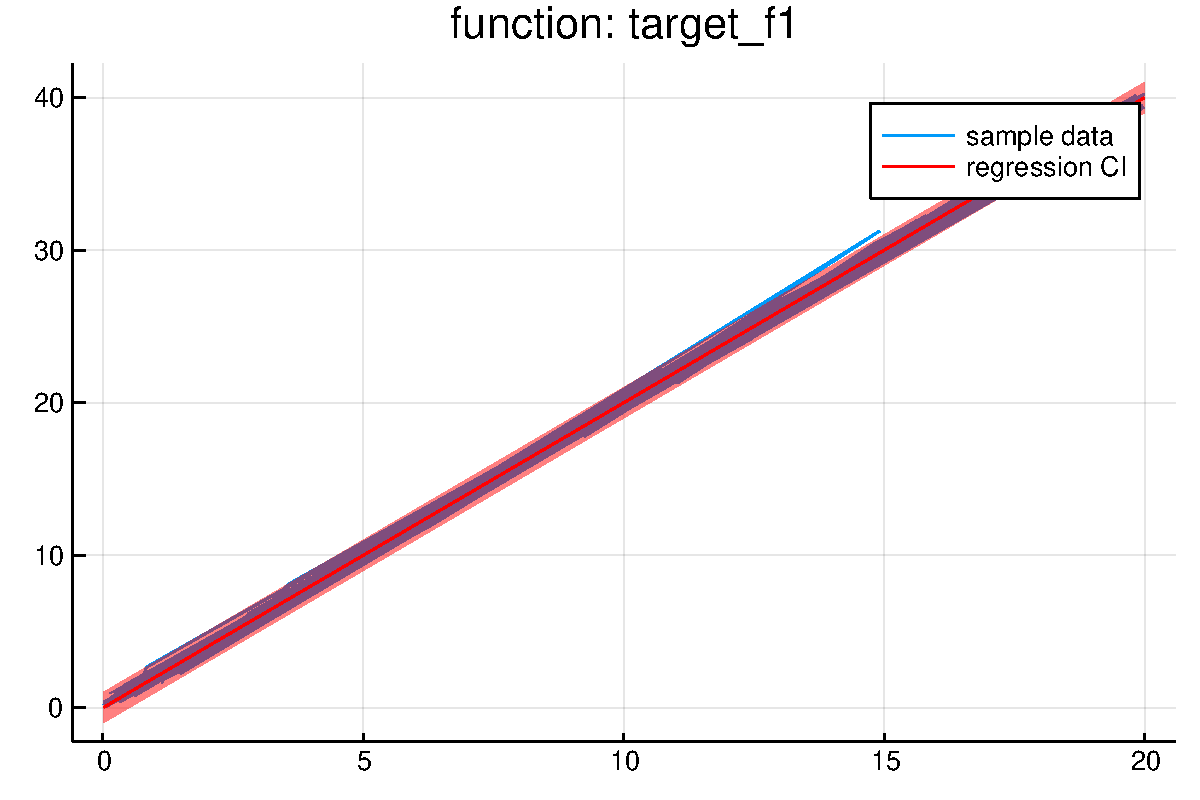
\includegraphics[width=\linewidth]{figures/A1_18_1.pdf}
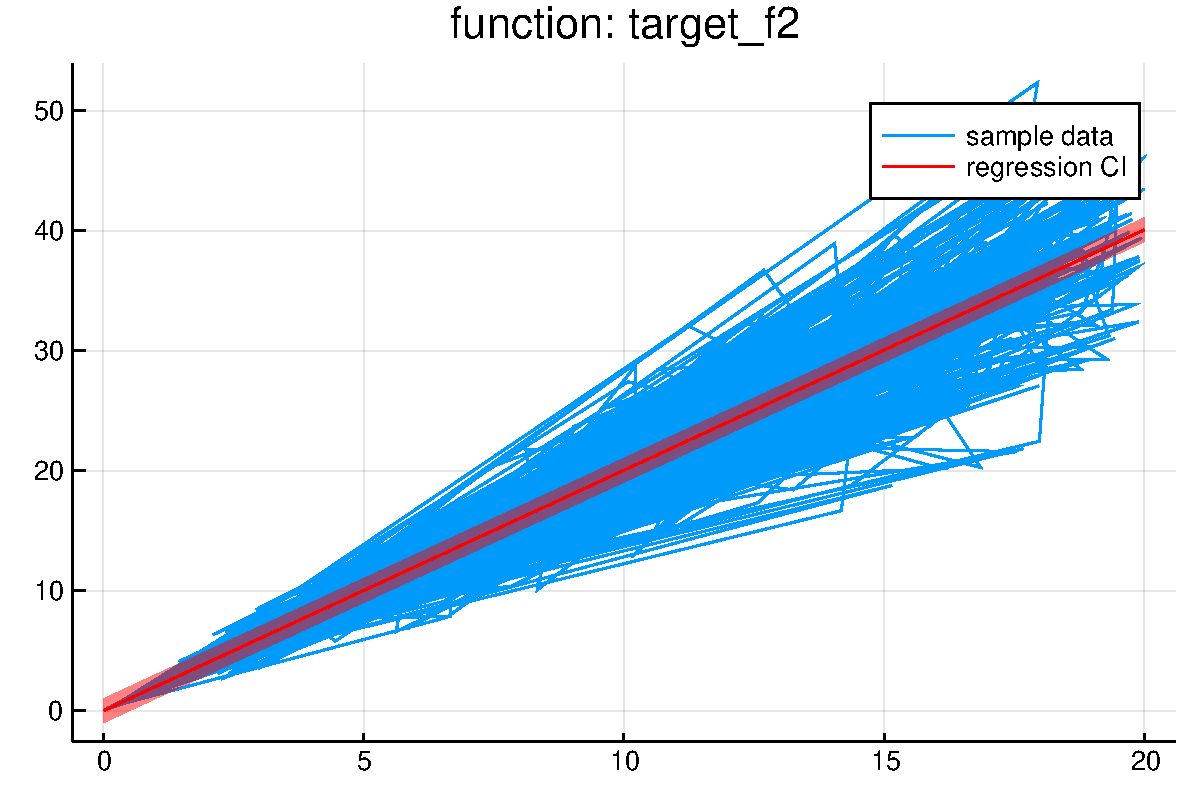
\includegraphics[width=\linewidth]{figures/A1_18_2.pdf}
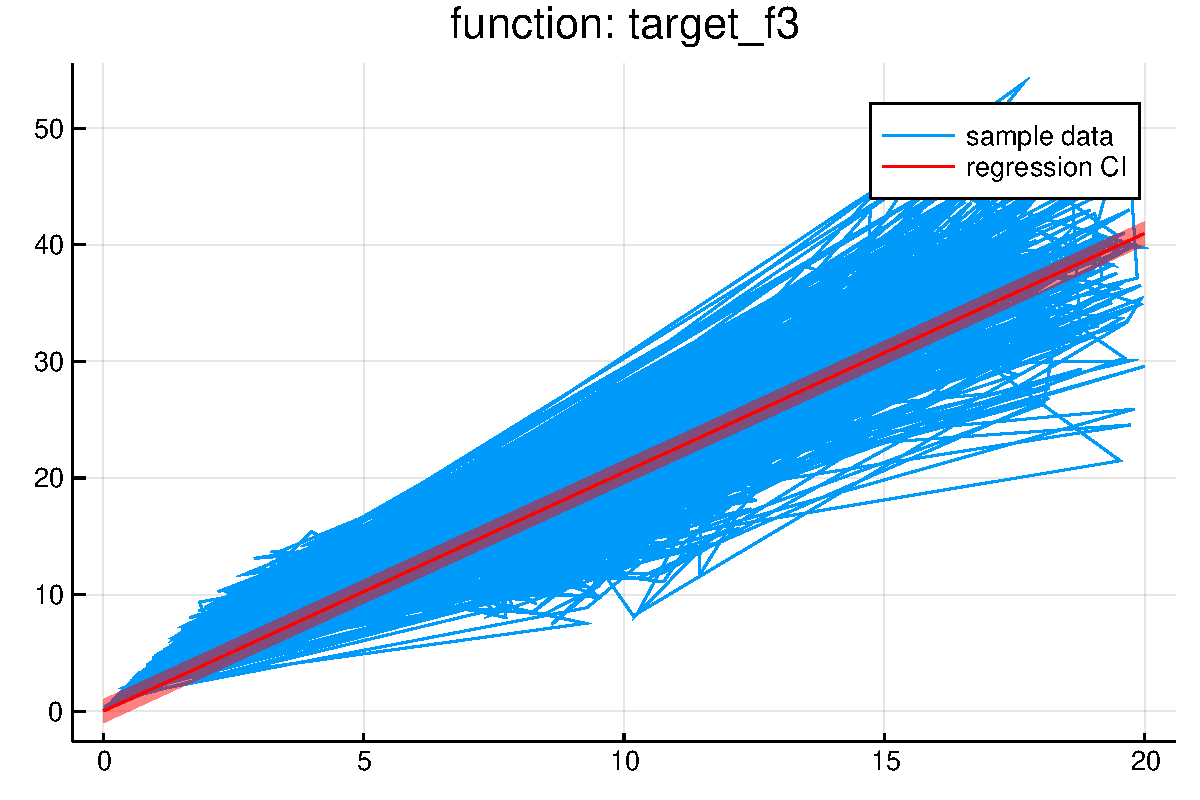
\includegraphics[width=\linewidth]{figures/A1_18_3.pdf}

\subsubsection{Non-linear Regression with a Neural Network [9pts]}
In the previous questions we have considered a linear regression model

\[
Y \sim \mathcal{N}(X^T \beta, \sigma^2)
\]
This model specified the mean of the predictive distribution for each datapoint by the product of that datapoint with our parameter.

Now, let us generalize this to consider a model where the mean of the predictive distribution is a non-linear function of each datapoint. We will have our non-linear model be a simple function called \texttt{neural\_net} with parameters $\theta$ (collection of weights and biases).

\[
Y \sim \mathcal{N}(\texttt{neural\_net}(X,\theta), \sigma^2)
\]
\begin{itemize}
\item[1. ] [3pts] Write the code for a fully-connected neural network (multi-layer perceptron) with one 10-dimensional hidden layer and a \texttt{tanh} nonlinearirty.  You must write this yourself using only basic operations like matrix multiply and \texttt{tanh}, you may not use layers provided by a library.

This network will output the mean vector, test that it outputs the correct shape for some random parameters.

\end{itemize}

\begin{lstlisting}
(*@\HLJLcs{{\#}}@*) (*@\HLJLcs{Neural}@*) (*@\HLJLcs{Network}@*) (*@\HLJLcs{Function}@*)
(*@\HLJLcs{{\#}x:1*n}@*)
(*@\HLJLk{function}@*) (*@\HLJLnf{neural{\_}net}@*)(*@\HLJLp{(}@*)(*@\HLJLn{x}@*)(*@\HLJLp{,}@*)(*@\HLJLn{\ensuremath{\theta}}@*)(*@\HLJLp{)}@*)
  (*@\HLJLn{W1}@*) (*@\HLJLoB{=}@*) (*@\HLJLn{\ensuremath{\theta}}@*)(*@\HLJLp{[}@*)(*@\HLJLni{1}@*)(*@\HLJLp{]}@*)
  (*@\HLJLn{b1}@*) (*@\HLJLoB{=}@*) (*@\HLJLn{\ensuremath{\theta}}@*)(*@\HLJLp{[}@*)(*@\HLJLni{2}@*)(*@\HLJLp{]}@*)
  (*@\HLJLn{W2}@*) (*@\HLJLoB{=}@*) (*@\HLJLn{\ensuremath{\theta}}@*)(*@\HLJLp{[}@*)(*@\HLJLni{3}@*)(*@\HLJLp{]}@*)
  (*@\HLJLn{b2}@*) (*@\HLJLoB{=}@*) (*@\HLJLn{\ensuremath{\theta}}@*)(*@\HLJLp{[}@*)(*@\HLJLni{4}@*)(*@\HLJLp{]}@*)
  (*@\HLJLn{H}@*) (*@\HLJLoB{=}@*) (*@\HLJLn{tanh}@*)(*@\HLJLoB{.}@*)(*@\HLJLp{(}@*)(*@\HLJLn{W1}@*)(*@\HLJLoB{*}@*)(*@\HLJLn{x}@*)(*@\HLJLoB{{\textquotesingle}}@*) (*@\HLJLoB{+}@*) (*@\HLJLn{b1}@*)(*@\HLJLp{)}@*)
  (*@\HLJLk{return}@*) (*@\HLJLn{W2}@*)(*@\HLJLoB{*}@*)(*@\HLJLn{H}@*) (*@\HLJLoB{+}@*) (*@\HLJLn{b2}@*)
(*@\HLJLk{end}@*)



(*@\HLJLcs{{\#}}@*) (*@\HLJLcs{Random}@*) (*@\HLJLcs{initial}@*) (*@\HLJLcs{Parameters}@*)
(*@\HLJLn{n}@*) (*@\HLJLoB{=}@*) (*@\HLJLni{100}@*)
(*@\HLJLn{\ensuremath{\theta}}@*) (*@\HLJLoB{=}@*) (*@\HLJLp{(}@*)(*@\HLJLnf{randn}@*)(*@\HLJLp{(}@*)(*@\HLJLni{10}@*)(*@\HLJLp{,}@*)(*@\HLJLn{n}@*)(*@\HLJLp{),}@*) (*@\HLJLnf{randn}@*)(*@\HLJLp{(}@*)(*@\HLJLni{10}@*)(*@\HLJLp{,),}@*)(*@\HLJLnf{randn}@*)(*@\HLJLp{(}@*)(*@\HLJLn{n}@*)(*@\HLJLp{,}@*)(*@\HLJLni{10}@*)(*@\HLJLp{),}@*)(*@\HLJLnf{randn}@*)(*@\HLJLp{(}@*)(*@\HLJLn{n}@*)(*@\HLJLp{,))}@*)
(*@\HLJLn{x}@*)(*@\HLJLp{,}@*)(*@\HLJLn{y}@*) (*@\HLJLoB{=}@*) (*@\HLJLnf{sample{\_}batch}@*)(*@\HLJLp{(}@*)(*@\HLJLn{target{\_}f1}@*)(*@\HLJLp{,}@*)(*@\HLJLn{n}@*)(*@\HLJLp{)}@*)
(*@\HLJLnd{@testset}@*) (*@\HLJLs{"{}neural}@*) (*@\HLJLs{net}@*) (*@\HLJLs{mean}@*) (*@\HLJLs{vector}@*) (*@\HLJLs{output"{}}@*) (*@\HLJLk{begin}@*)
(*@\HLJLn{x}@*)(*@\HLJLp{,}@*)(*@\HLJLn{y}@*) (*@\HLJLoB{=}@*) (*@\HLJLnf{sample{\_}batch}@*)(*@\HLJLp{(}@*)(*@\HLJLn{target{\_}f1}@*)(*@\HLJLp{,}@*)(*@\HLJLn{n}@*)(*@\HLJLp{)}@*)
(*@\HLJLn{\ensuremath{\mu}}@*) (*@\HLJLoB{=}@*) (*@\HLJLnf{neural{\_}net}@*)(*@\HLJLp{(}@*)(*@\HLJLn{x}@*)(*@\HLJLp{,}@*)(*@\HLJLn{\ensuremath{\theta}}@*)(*@\HLJLp{)}@*)
(*@\HLJLnd{@test}@*) (*@\HLJLnf{size}@*)(*@\HLJLp{(}@*)(*@\HLJLn{\ensuremath{\mu}}@*)(*@\HLJLp{)}@*) (*@\HLJLoB{==}@*) (*@\HLJLp{(}@*)(*@\HLJLn{n}@*)(*@\HLJLp{,)}@*)
(*@\HLJLk{end}@*)
\end{lstlisting}

\begin{lstlisting}
Test Summary:                 | Pass  Total
neural net mean vector output |    1      1
Test.DefaultTestSet("neural net mean vector output", Any[], 1, false)
\end{lstlisting}


\begin{itemize}
\item[2. ] [2pts] Write the code that computes the negative log-likelihood for this model where the mean is given by the output of the neural network and $\sigma = 1.0$

\end{itemize}

\begin{lstlisting}
(*@\HLJLcs{{\#}x}@*) (*@\HLJLcs{is}@*) (*@\HLJLcs{1*n,}@*) (*@\HLJLcs{y}@*) (*@\HLJLcs{is}@*) (*@\HLJLcs{n*1}@*)
(*@\HLJLk{function}@*) (*@\HLJLnf{nn{\_}model{\_}nll}@*)(*@\HLJLp{(}@*)(*@\HLJLn{\ensuremath{\theta}}@*)(*@\HLJLp{,}@*)(*@\HLJLn{x}@*)(*@\HLJLp{,}@*)(*@\HLJLn{y}@*)(*@\HLJLp{;}@*)(*@\HLJLn{\ensuremath{\sigma}}@*)(*@\HLJLoB{=}@*)(*@\HLJLni{1}@*)(*@\HLJLp{)}@*)
  (*@\HLJLn{\ensuremath{\mu}}@*) (*@\HLJLoB{=}@*) (*@\HLJLnf{neural{\_}net}@*)(*@\HLJLp{(}@*)(*@\HLJLn{x}@*)(*@\HLJLp{,}@*)(*@\HLJLn{\ensuremath{\theta}}@*)(*@\HLJLp{)}@*)
  (*@\HLJLk{return}@*) (*@\HLJLoB{-}@*)(*@\HLJLnf{sum}@*)(*@\HLJLp{(}@*)(*@\HLJLn{gaussian{\_}log{\_}likelihood}@*)(*@\HLJLoB{.}@*)(*@\HLJLp{(}@*)(*@\HLJLn{\ensuremath{\mu}}@*)(*@\HLJLp{,}@*) (*@\HLJLn{\ensuremath{\sigma}}@*)(*@\HLJLp{,}@*) (*@\HLJLn{y}@*)(*@\HLJLp{))}@*)
(*@\HLJLk{end}@*)
\end{lstlisting}

\begin{lstlisting}
nn_model_nll (generic function with 1 method)
\end{lstlisting}


\begin{itemize}
\item[3. ] [2pts] Write a function \texttt{train\_nn\_reg} that accepts a target function and an initial estimate for $\theta$ and some  hyperparameters for batch-size, model variance, learning rate, and number of iterations.  Then, for each iteration:

\begin{itemize}
\item sample data from the target function


\item compute gradients of negative log-likelihood with respect to $\theta$


\item update the estimate of $\theta$ with gradient descent with specified learning rate

\end{itemize}
and, after all iterations, returns the final estimate of $\theta$.

\end{itemize}

\begin{lstlisting}
(*@\HLJLk{using}@*) (*@\HLJLn{Logging}@*) (*@\HLJLcs{{\#}}@*) (*@\HLJLcs{Print}@*) (*@\HLJLcs{training}@*) (*@\HLJLcs{progress}@*) (*@\HLJLcs{to}@*) (*@\HLJLcs{REPL,}@*) (*@\HLJLcs{not}@*) (*@\HLJLcs{pdf}@*)

(*@\HLJLk{function}@*) (*@\HLJLnf{train{\_}nn{\_}reg}@*)(*@\HLJLp{(}@*)(*@\HLJLn{target{\_}f}@*)(*@\HLJLp{,}@*) (*@\HLJLn{\ensuremath{\theta}{\_}init}@*)(*@\HLJLp{;}@*) (*@\HLJLn{bs}@*)(*@\HLJLoB{=}@*) (*@\HLJLni{100}@*)(*@\HLJLp{,}@*) (*@\HLJLn{lr}@*) (*@\HLJLoB{=}@*) (*@\HLJLnfB{1e-5}@*)(*@\HLJLp{,}@*) (*@\HLJLn{iters}@*)(*@\HLJLoB{=}@*)(*@\HLJLni{1000}@*)(*@\HLJLp{,}@*) (*@\HLJLn{\ensuremath{\sigma}{\_}model}@*) (*@\HLJLoB{=}@*) (*@\HLJLnfB{1.}@*) (*@\HLJLp{)}@*)
    (*@\HLJLn{\ensuremath{\theta}{\_}curr}@*) (*@\HLJLoB{=}@*) (*@\HLJLn{\ensuremath{\theta}{\_}init}@*)
    (*@\HLJLk{for}@*) (*@\HLJLn{i}@*) (*@\HLJLkp{in}@*) (*@\HLJLni{1}@*)(*@\HLJLoB{:}@*)(*@\HLJLn{iters}@*)
      (*@\HLJLn{x}@*)(*@\HLJLp{,}@*)(*@\HLJLn{y}@*) (*@\HLJLoB{=}@*) (*@\HLJLnf{sample{\_}batch}@*)(*@\HLJLp{(}@*)(*@\HLJLn{target{\_}f}@*)(*@\HLJLp{,}@*) (*@\HLJLn{bs}@*)(*@\HLJLp{)}@*)
      (*@\HLJLn{log{\_}loss}@*) (*@\HLJLoB{=}@*) (*@\HLJLnf{nn{\_}model{\_}nll}@*)(*@\HLJLp{(}@*)(*@\HLJLn{\ensuremath{\theta}{\_}curr}@*)(*@\HLJLp{,}@*) (*@\HLJLn{x}@*)(*@\HLJLp{,}@*) (*@\HLJLn{y}@*)(*@\HLJLp{)}@*)
      (*@\HLJLnd{@info}@*) (*@\HLJLs{"{}loss:}@*) (*@\HLJLsi{{\$}log{\_}loss}@*)(*@\HLJLs{"{}}@*) (*@\HLJLcs{{\#}TODO:}@*) (*@\HLJLcs{log}@*) (*@\HLJLcs{loss,}@*) (*@\HLJLcs{if}@*) (*@\HLJLcs{you}@*) (*@\HLJLcs{want}@*) (*@\HLJLcs{to}@*) (*@\HLJLcs{montior}@*) (*@\HLJLcs{training}@*)
      (*@\HLJLn{grad{\_}\ensuremath{\theta}}@*) (*@\HLJLoB{=}@*) (*@\HLJLnf{gradient}@*)(*@\HLJLp{((}@*)(*@\HLJLn{\ensuremath{\theta}}@*) (*@\HLJLoB{->}@*) (*@\HLJLnf{nn{\_}model{\_}nll}@*)(*@\HLJLp{(}@*)(*@\HLJLn{\ensuremath{\theta}}@*)(*@\HLJLp{,}@*)(*@\HLJLn{x}@*)(*@\HLJLp{,}@*)(*@\HLJLn{y}@*)(*@\HLJLp{;}@*) (*@\HLJLn{\ensuremath{\sigma}}@*) (*@\HLJLoB{=}@*) (*@\HLJLn{\ensuremath{\sigma}{\_}model}@*)(*@\HLJLp{)),}@*) (*@\HLJLn{\ensuremath{\theta}{\_}curr}@*)(*@\HLJLp{)[}@*)(*@\HLJLni{1}@*)(*@\HLJLp{]}@*)
      (*@\HLJLcs{{\#}:}@*) (*@\HLJLcs{compute}@*) (*@\HLJLcs{gradients}@*)
      (*@\HLJLk{for}@*) (*@\HLJLn{j}@*) (*@\HLJLkp{in}@*) (*@\HLJLni{1}@*)(*@\HLJLoB{:}@*)(*@\HLJLni{4}@*)
        (*@\HLJLn{\ensuremath{\theta}{\_}curr}@*)(*@\HLJLp{[}@*)(*@\HLJLn{j}@*)(*@\HLJLp{]}@*) (*@\HLJLoB{=}@*) (*@\HLJLn{\ensuremath{\theta}{\_}curr}@*)(*@\HLJLp{[}@*)(*@\HLJLn{j}@*)(*@\HLJLp{]}@*) (*@\HLJLoB{-}@*) (*@\HLJLn{lr}@*)(*@\HLJLoB{*}@*)(*@\HLJLn{grad{\_}\ensuremath{\theta}}@*)(*@\HLJLp{[}@*)(*@\HLJLn{j}@*)(*@\HLJLp{]}@*)(*@\HLJLcs{{\#}:gradient}@*) (*@\HLJLcs{descent}@*)
      (*@\HLJLk{end}@*)
    (*@\HLJLk{end}@*)
    (*@\HLJLk{return}@*) (*@\HLJLn{\ensuremath{\theta}{\_}curr}@*)
(*@\HLJLk{end}@*)
\end{lstlisting}

\begin{lstlisting}
train_nn_reg (generic function with 1 method)
\end{lstlisting}


\begin{itemize}
\item[4. ] [2pts]

\end{itemize}

\begin{lstlisting}
(*@\HLJLk{using}@*) (*@\HLJLn{Zygote}@*)(*@\HLJLoB{:}@*)(*@\HLJLn{gradient}@*)
(*@\HLJLn{n}@*) (*@\HLJLoB{=}@*) (*@\HLJLni{1000}@*)
(*@\HLJLn{m}@*) (*@\HLJLoB{=}@*) (*@\HLJLni{100}@*)
(*@\HLJLcs{{\#}TODO:}@*) (*@\HLJLcs{For}@*) (*@\HLJLcs{each}@*) (*@\HLJLcs{target}@*) (*@\HLJLcs{function}@*)
(*@\HLJLk{for}@*) (*@\HLJLn{target{\_}f}@*) (*@\HLJLkp{in}@*) (*@\HLJLp{(}@*)(*@\HLJLn{target{\_}f1}@*)(*@\HLJLp{,}@*) (*@\HLJLn{target{\_}f2}@*)(*@\HLJLp{,}@*) (*@\HLJLn{target{\_}f3}@*)(*@\HLJLp{)}@*)
  (*@\HLJLn{\ensuremath{\theta}{\_}init}@*) (*@\HLJLoB{=}@*) (*@\HLJLp{(}@*)(*@\HLJLnf{rand}@*)(*@\HLJLp{(}@*)(*@\HLJLni{10}@*)(*@\HLJLp{,}@*)(*@\HLJLn{m}@*)(*@\HLJLp{),}@*) (*@\HLJLnf{randn}@*)(*@\HLJLp{(}@*)(*@\HLJLni{10}@*)(*@\HLJLp{,),}@*)(*@\HLJLnf{rand}@*)(*@\HLJLp{(}@*)(*@\HLJLn{m}@*)(*@\HLJLp{,}@*)(*@\HLJLni{10}@*)(*@\HLJLp{),}@*)(*@\HLJLnf{randn}@*)(*@\HLJLp{(}@*)(*@\HLJLn{m}@*)(*@\HLJLp{,))}@*)
  (*@\HLJLn{\ensuremath{\theta}{\_}learned}@*) (*@\HLJLoB{=}@*) (*@\HLJLnf{train{\_}nn{\_}reg}@*)(*@\HLJLp{(}@*)(*@\HLJLn{target{\_}f}@*)(*@\HLJLp{,}@*) (*@\HLJLn{\ensuremath{\theta}{\_}init}@*)(*@\HLJLp{)}@*)
  (*@\HLJLn{x}@*)(*@\HLJLp{,}@*)(*@\HLJLn{y}@*) (*@\HLJLoB{=}@*) (*@\HLJLnf{sample{\_}batch}@*)(*@\HLJLp{(}@*)(*@\HLJLn{target{\_}f}@*)(*@\HLJLp{,}@*) (*@\HLJLn{n}@*)(*@\HLJLp{)}@*)
  (*@\HLJLnf{plot}@*)(*@\HLJLp{(}@*)(*@\HLJLn{x}@*)(*@\HLJLoB{{\textquotesingle}}@*)(*@\HLJLp{,}@*)(*@\HLJLn{y}@*)(*@\HLJLp{,}@*) (*@\HLJLn{label}@*) (*@\HLJLoB{=}@*) (*@\HLJLs{"{}sample}@*) (*@\HLJLs{data"{}}@*)(*@\HLJLp{,}@*) (*@\HLJLn{title}@*) (*@\HLJLoB{=}@*) (*@\HLJLs{"{}function:}@*) (*@\HLJLsi{{\$}target{\_}f}@*)(*@\HLJLs{"{}}@*)(*@\HLJLp{)}@*)
  (*@\HLJLnf{sort!}@*)(*@\HLJLp{(}@*)(*@\HLJLn{x}@*)(*@\HLJLoB{{\textquotesingle}}@*)(*@\HLJLp{)}@*)
  (*@\HLJLnf{display}@*)(*@\HLJLp{(}@*)(*@\HLJLnf{plot!}@*)(*@\HLJLp{(}@*)(*@\HLJLn{x}@*)(*@\HLJLoB{{\textquotesingle}}@*)(*@\HLJLp{,}@*) (*@\HLJLn{x}@*)(*@\HLJLoB{{\textquotesingle}}@*) (*@\HLJLoB{*}@*) (*@\HLJLn{\ensuremath{\theta}{\_}learned}@*)(*@\HLJLp{,}@*) (*@\HLJLn{color}@*) (*@\HLJLoB{=}@*) (*@\HLJLs{"{}red"{}}@*)(*@\HLJLp{,}@*) (*@\HLJLn{ribbon}@*) (*@\HLJLoB{=}@*) (*@\HLJLni{1}@*)(*@\HLJLp{,}@*) (*@\HLJLn{label}@*) (*@\HLJLoB{=}@*) (*@\HLJLs{"{}regression}@*) (*@\HLJLs{CI"{}}@*)(*@\HLJLp{))}@*)
(*@\HLJLk{end}@*)
\end{lstlisting}

\begin{lstlisting}
Error: MethodError: no method matching setindex!(::Tuple{Array{Float64,2},A
rray{Float64,1},Array{Float64,2},Array{Float64,1}}, ::Array{Float64,2}, ::I
nt64)
\end{lstlisting}


\begin{lstlisting}
(*@\HLJLcs{{\#}TODO:}@*) (*@\HLJLcs{plot}@*) (*@\HLJLcs{data}@*) (*@\HLJLcs{samples}@*) (*@\HLJLcs{and}@*) (*@\HLJLcs{learned}@*) (*@\HLJLcs{regression}@*)
\end{lstlisting}


\subsubsection{Non-linear Regression and Input-dependent Variance with a Neural Network}

\begin{align*}
\mu, \log \sigma &= \texttt{neural\_net}(X,\theta)\\
Y &\sim \mathcal{N}(\mu, \exp(\log \sigma)^2)
\end{align*}
\begin{itemize}
\item[1. ] [1pts]

\end{itemize}

\begin{lstlisting}
(*@\HLJLcs{{\#}}@*) (*@\HLJLcs{Neural}@*) (*@\HLJLcs{Network}@*) (*@\HLJLcs{Function}@*)
(*@\HLJLk{function}@*) (*@\HLJLnf{neural{\_}net{\_}w{\_}var}@*)(*@\HLJLp{(}@*)(*@\HLJLn{x}@*)(*@\HLJLp{,}@*)(*@\HLJLn{\ensuremath{\theta}}@*)(*@\HLJLp{)}@*)
  (*@\HLJLn{W11}@*) (*@\HLJLoB{=}@*) (*@\HLJLn{\ensuremath{\theta}}@*)(*@\HLJLp{[}@*)(*@\HLJLni{1}@*)(*@\HLJLp{]}@*)
  (*@\HLJLn{b11}@*) (*@\HLJLoB{=}@*) (*@\HLJLn{\ensuremath{\theta}}@*)(*@\HLJLp{[}@*)(*@\HLJLni{2}@*)(*@\HLJLp{]}@*)
  (*@\HLJLn{W12}@*) (*@\HLJLoB{=}@*) (*@\HLJLn{\ensuremath{\theta}}@*)(*@\HLJLp{[}@*)(*@\HLJLni{3}@*)(*@\HLJLp{]}@*)
  (*@\HLJLn{b12}@*) (*@\HLJLoB{=}@*) (*@\HLJLn{\ensuremath{\theta}}@*)(*@\HLJLp{[}@*)(*@\HLJLni{4}@*)(*@\HLJLp{]}@*)
  (*@\HLJLn{W21}@*) (*@\HLJLoB{=}@*) (*@\HLJLn{\ensuremath{\theta}}@*)(*@\HLJLp{[}@*)(*@\HLJLni{5}@*)(*@\HLJLp{]}@*)
  (*@\HLJLn{b21}@*) (*@\HLJLoB{=}@*) (*@\HLJLn{\ensuremath{\theta}}@*)(*@\HLJLp{[}@*)(*@\HLJLni{6}@*)(*@\HLJLp{]}@*)
  (*@\HLJLn{W22}@*) (*@\HLJLoB{=}@*) (*@\HLJLn{\ensuremath{\theta}}@*)(*@\HLJLp{[}@*)(*@\HLJLni{7}@*)(*@\HLJLp{]}@*)
  (*@\HLJLn{b22}@*) (*@\HLJLoB{=}@*) (*@\HLJLn{\ensuremath{\theta}}@*)(*@\HLJLp{[}@*)(*@\HLJLni{8}@*)(*@\HLJLp{]}@*)
  (*@\HLJLn{H1}@*) (*@\HLJLoB{=}@*) (*@\HLJLn{tanh}@*)(*@\HLJLoB{.}@*)(*@\HLJLp{(}@*)(*@\HLJLn{W11}@*)(*@\HLJLoB{*}@*)(*@\HLJLn{x}@*)(*@\HLJLoB{{\textquotesingle}}@*) (*@\HLJLoB{+}@*) (*@\HLJLn{b11}@*)(*@\HLJLp{)}@*)
  (*@\HLJLn{\ensuremath{\mu}{\_}hat}@*) (*@\HLJLoB{=}@*) (*@\HLJLn{W12}@*)(*@\HLJLoB{*}@*)(*@\HLJLn{H1}@*) (*@\HLJLoB{+}@*) (*@\HLJLn{b12}@*)
  (*@\HLJLn{H2}@*) (*@\HLJLoB{=}@*) (*@\HLJLn{tanh}@*)(*@\HLJLoB{.}@*)(*@\HLJLp{(}@*)(*@\HLJLn{W21}@*)(*@\HLJLoB{*}@*)(*@\HLJLn{x}@*)(*@\HLJLoB{{\textquotesingle}}@*) (*@\HLJLoB{+}@*) (*@\HLJLn{b21}@*)(*@\HLJLp{)}@*)
  (*@\HLJLn{log{\_}\ensuremath{\sigma}}@*) (*@\HLJLoB{=}@*) (*@\HLJLn{W22}@*)(*@\HLJLoB{*}@*)(*@\HLJLn{H2}@*) (*@\HLJLoB{+}@*) (*@\HLJLn{b22}@*)
  (*@\HLJLk{return}@*) (*@\HLJLp{(}@*)(*@\HLJLn{\ensuremath{\mu}{\_}hat}@*)(*@\HLJLp{,}@*) (*@\HLJLn{log{\_}\ensuremath{\sigma}}@*)(*@\HLJLp{)}@*)
(*@\HLJLk{end}@*)


(*@\HLJLnd{@testset}@*) (*@\HLJLs{"{}neural}@*) (*@\HLJLs{net}@*) (*@\HLJLs{mean}@*) (*@\HLJLs{and}@*) (*@\HLJLs{logsigma}@*) (*@\HLJLs{vector}@*) (*@\HLJLs{output"{}}@*) (*@\HLJLk{begin}@*)
(*@\HLJLn{n}@*) (*@\HLJLoB{=}@*) (*@\HLJLni{100}@*)
(*@\HLJLn{\ensuremath{\theta}}@*) (*@\HLJLoB{=}@*) (*@\HLJLp{(}@*)(*@\HLJLnf{rand}@*)(*@\HLJLp{(}@*)(*@\HLJLni{10}@*)(*@\HLJLp{,}@*)(*@\HLJLn{n}@*)(*@\HLJLp{),}@*) (*@\HLJLnf{randn}@*)(*@\HLJLp{(}@*)(*@\HLJLni{10}@*)(*@\HLJLp{,),}@*)(*@\HLJLnf{rand}@*)(*@\HLJLp{(}@*)(*@\HLJLn{n}@*)(*@\HLJLp{,}@*)(*@\HLJLni{10}@*)(*@\HLJLp{),}@*)(*@\HLJLnf{randn}@*)(*@\HLJLp{(}@*)(*@\HLJLn{n}@*)(*@\HLJLp{,),}@*)
    (*@\HLJLnf{rand}@*)(*@\HLJLp{(}@*)(*@\HLJLni{10}@*)(*@\HLJLp{,}@*)(*@\HLJLn{n}@*)(*@\HLJLp{),}@*) (*@\HLJLnf{randn}@*)(*@\HLJLp{(}@*)(*@\HLJLni{10}@*)(*@\HLJLp{,),}@*)(*@\HLJLnf{rand}@*)(*@\HLJLp{(}@*)(*@\HLJLn{n}@*)(*@\HLJLp{,}@*)(*@\HLJLni{10}@*)(*@\HLJLp{),}@*)(*@\HLJLnf{randn}@*)(*@\HLJLp{(}@*)(*@\HLJLn{n}@*)(*@\HLJLp{,))}@*)
(*@\HLJLn{x}@*)(*@\HLJLp{,}@*)(*@\HLJLn{y}@*) (*@\HLJLoB{=}@*) (*@\HLJLnf{sample{\_}batch}@*)(*@\HLJLp{(}@*)(*@\HLJLn{target{\_}f1}@*)(*@\HLJLp{,}@*)(*@\HLJLn{n}@*)(*@\HLJLp{)}@*)
(*@\HLJLn{\ensuremath{\mu}}@*)(*@\HLJLp{,}@*) (*@\HLJLn{log\ensuremath{\sigma}}@*) (*@\HLJLoB{=}@*) (*@\HLJLnf{neural{\_}net{\_}w{\_}var}@*)(*@\HLJLp{(}@*)(*@\HLJLn{x}@*)(*@\HLJLp{,}@*)(*@\HLJLn{\ensuremath{\theta}}@*)(*@\HLJLp{)}@*)
(*@\HLJLnd{@test}@*) (*@\HLJLnf{size}@*)(*@\HLJLp{(}@*)(*@\HLJLn{\ensuremath{\mu}}@*)(*@\HLJLp{)}@*) (*@\HLJLoB{==}@*) (*@\HLJLp{(}@*)(*@\HLJLn{n}@*)(*@\HLJLp{,)}@*)
(*@\HLJLnd{@test}@*) (*@\HLJLnf{size}@*)(*@\HLJLp{(}@*)(*@\HLJLn{log\ensuremath{\sigma}}@*)(*@\HLJLp{)}@*) (*@\HLJLoB{==}@*) (*@\HLJLp{(}@*)(*@\HLJLn{n}@*)(*@\HLJLp{,)}@*)
(*@\HLJLk{end}@*)
\end{lstlisting}

\begin{lstlisting}
Test Summary:                              | Pass  Total
neural net mean and logsigma vector output |    2      2
Test.DefaultTestSet("neural net mean and logsigma vector output", Any[], 2,
 false)
\end{lstlisting}


\begin{itemize}
\item[2. ] [2pts]

\end{itemize}

\begin{lstlisting}
(*@\HLJLk{function}@*) (*@\HLJLnf{nn{\_}with{\_}var{\_}model{\_}nll}@*)(*@\HLJLp{(}@*)(*@\HLJLn{\ensuremath{\theta}}@*)(*@\HLJLp{,}@*)(*@\HLJLn{x}@*)(*@\HLJLp{,}@*)(*@\HLJLn{y}@*)(*@\HLJLp{)}@*)
  (*@\HLJLn{\ensuremath{\mu}}@*)(*@\HLJLp{,}@*)(*@\HLJLn{log{\_}\ensuremath{\sigma}}@*) (*@\HLJLoB{=}@*) (*@\HLJLnf{neural{\_}net{\_}w{\_}var}@*)(*@\HLJLp{(}@*)(*@\HLJLn{x}@*)(*@\HLJLp{,}@*) (*@\HLJLn{\ensuremath{\theta}}@*)(*@\HLJLp{)}@*)
  (*@\HLJLn{\ensuremath{\sigma}}@*) (*@\HLJLoB{=}@*) (*@\HLJLnf{exp}@*)(*@\HLJLp{(}@*)(*@\HLJLn{log{\_}\ensuremath{\sigma}}@*)(*@\HLJLp{)}@*)
  (*@\HLJLk{return}@*) (*@\HLJLk{return}@*) (*@\HLJLoB{-}@*)(*@\HLJLnf{sum}@*)(*@\HLJLp{(}@*)(*@\HLJLn{gaussian{\_}log{\_}likelihood}@*)(*@\HLJLoB{.}@*)(*@\HLJLp{(}@*)(*@\HLJLn{\ensuremath{\mu}}@*)(*@\HLJLp{,}@*) (*@\HLJLn{\ensuremath{\sigma}}@*)(*@\HLJLp{,}@*) (*@\HLJLn{y}@*)(*@\HLJLp{))}@*)
(*@\HLJLk{end}@*)
\end{lstlisting}

\begin{lstlisting}
nn_with_var_model_nll (generic function with 1 method)
\end{lstlisting}


\begin{itemize}
\item[3. ] [1pts]

\end{itemize}

\begin{lstlisting}
(*@\HLJLk{function}@*) (*@\HLJLnf{train{\_}nn{\_}w{\_}var{\_}reg}@*)(*@\HLJLp{(}@*)(*@\HLJLn{target{\_}f}@*)(*@\HLJLp{,}@*) (*@\HLJLn{\ensuremath{\theta}{\_}init}@*)(*@\HLJLp{;}@*) (*@\HLJLn{bs}@*)(*@\HLJLoB{=}@*) (*@\HLJLni{100}@*)(*@\HLJLp{,}@*) (*@\HLJLn{lr}@*) (*@\HLJLoB{=}@*) (*@\HLJLnfB{1e-4}@*)(*@\HLJLp{,}@*) (*@\HLJLn{iters}@*)(*@\HLJLoB{=}@*)(*@\HLJLni{10000}@*)(*@\HLJLp{)}@*)
    (*@\HLJLn{\ensuremath{\theta}{\_}curr}@*) (*@\HLJLoB{=}@*) (*@\HLJLn{\ensuremath{\theta}{\_}init}@*)
    (*@\HLJLk{for}@*) (*@\HLJLn{i}@*) (*@\HLJLkp{in}@*) (*@\HLJLni{1}@*)(*@\HLJLoB{:}@*)(*@\HLJLn{iters}@*)
      (*@\HLJLn{x}@*)(*@\HLJLp{,}@*)(*@\HLJLn{y}@*) (*@\HLJLoB{=}@*) (*@\HLJLnf{sample{\_}batch}@*)(*@\HLJLp{(}@*)(*@\HLJLn{target{\_}f}@*)(*@\HLJLp{,}@*) (*@\HLJLn{bs}@*)(*@\HLJLp{)}@*)
      (*@\HLJLn{log{\_}loss}@*) (*@\HLJLoB{=}@*) (*@\HLJLnf{nn{\_}with{\_}var{\_}model{\_}nll}@*)(*@\HLJLp{(}@*)(*@\HLJLn{\ensuremath{\theta}{\_}curr}@*)(*@\HLJLp{,}@*) (*@\HLJLn{x}@*)(*@\HLJLp{,}@*) (*@\HLJLn{y}@*)(*@\HLJLp{)}@*)
      (*@\HLJLnd{@info}@*) (*@\HLJLs{"{}loss:}@*) (*@\HLJLsi{{\$}log{\_}loss}@*)(*@\HLJLs{"{}}@*) (*@\HLJLcs{{\#}TODO:}@*) (*@\HLJLcs{log}@*) (*@\HLJLcs{loss}@*)
      (*@\HLJLn{grad{\_}\ensuremath{\theta}}@*) (*@\HLJLoB{=}@*) (*@\HLJLnf{gradient}@*)(*@\HLJLp{((}@*)(*@\HLJLn{\ensuremath{\theta}}@*) (*@\HLJLoB{->}@*) (*@\HLJLnf{nn{\_}with{\_}var{\_}model{\_}nll}@*)(*@\HLJLp{(}@*)(*@\HLJLn{\ensuremath{\theta}}@*)(*@\HLJLp{,}@*) (*@\HLJLn{x}@*)(*@\HLJLp{,}@*) (*@\HLJLn{y}@*)(*@\HLJLp{),}@*) (*@\HLJLn{\ensuremath{\theta}{\_}curr}@*)(*@\HLJLp{))[}@*)(*@\HLJLni{1}@*)(*@\HLJLp{]}@*) (*@\HLJLcs{{\#}compute}@*) (*@\HLJLcs{gradients}@*)
      (*@\HLJLk{for}@*) (*@\HLJLn{j}@*) (*@\HLJLkp{in}@*) (*@\HLJLni{1}@*)(*@\HLJLoB{:}@*)(*@\HLJLni{8}@*)
        (*@\HLJLn{\ensuremath{\theta}{\_}curr}@*)(*@\HLJLp{[}@*)(*@\HLJLn{j}@*)(*@\HLJLp{]}@*) (*@\HLJLoB{=}@*) (*@\HLJLn{\ensuremath{\theta}{\_}curr}@*)(*@\HLJLp{[}@*)(*@\HLJLn{j}@*)(*@\HLJLp{]}@*) (*@\HLJLoB{-}@*) (*@\HLJLn{lr}@*)(*@\HLJLoB{*}@*)(*@\HLJLn{grad{\_}\ensuremath{\theta}}@*)(*@\HLJLp{[}@*)(*@\HLJLn{j}@*)(*@\HLJLp{]}@*)(*@\HLJLcs{{\#}:gradient}@*) (*@\HLJLcs{descent}@*) (*@\HLJLcs{end}@*)
      (*@\HLJLk{end}@*)
    (*@\HLJLk{end}@*)
    (*@\HLJLk{return}@*) (*@\HLJLn{\ensuremath{\theta}{\_}curr}@*)
(*@\HLJLk{end}@*)
\end{lstlisting}

\begin{lstlisting}
train_nn_w_var_reg (generic function with 1 method)
\end{lstlisting}


\begin{itemize}
\item[4. ] [4pts]

\end{itemize}

\begin{lstlisting}
(*@\HLJLn{n}@*) (*@\HLJLoB{=}@*) (*@\HLJLni{1000}@*)
(*@\HLJLn{m}@*) (*@\HLJLoB{=}@*) (*@\HLJLni{100}@*)
(*@\HLJLk{for}@*) (*@\HLJLn{target{\_}f}@*) (*@\HLJLkp{in}@*) (*@\HLJLp{(}@*)(*@\HLJLn{target{\_}f1}@*)(*@\HLJLp{,}@*) (*@\HLJLn{target{\_}f2}@*)(*@\HLJLp{,}@*) (*@\HLJLn{target{\_}f3}@*)(*@\HLJLp{)}@*)
  (*@\HLJLn{\ensuremath{\theta}{\_}init}@*) (*@\HLJLoB{=}@*) (*@\HLJLp{(}@*)(*@\HLJLnf{rand}@*)(*@\HLJLp{(}@*)(*@\HLJLni{10}@*)(*@\HLJLp{,}@*)(*@\HLJLn{m}@*)(*@\HLJLp{),}@*) (*@\HLJLnf{randn}@*)(*@\HLJLp{(}@*)(*@\HLJLni{10}@*)(*@\HLJLp{,),}@*)(*@\HLJLnf{rand}@*)(*@\HLJLp{(}@*)(*@\HLJLn{m}@*)(*@\HLJLp{,}@*)(*@\HLJLni{10}@*)(*@\HLJLp{),}@*)(*@\HLJLnf{randn}@*)(*@\HLJLp{(}@*)(*@\HLJLn{m}@*)(*@\HLJLp{,))}@*)
  (*@\HLJLn{\ensuremath{\theta}{\_}learned}@*) (*@\HLJLoB{=}@*) (*@\HLJLnf{train{\_}nn{\_}w{\_}var{\_}reg}@*)(*@\HLJLp{(}@*)(*@\HLJLn{target{\_}f}@*)(*@\HLJLp{,}@*) (*@\HLJLn{\ensuremath{\theta}{\_}init}@*)(*@\HLJLp{)}@*)
  (*@\HLJLn{x}@*)(*@\HLJLp{,}@*)(*@\HLJLn{y}@*) (*@\HLJLoB{=}@*) (*@\HLJLnf{sample{\_}batch}@*)(*@\HLJLp{(}@*)(*@\HLJLn{target{\_}f}@*)(*@\HLJLp{,}@*) (*@\HLJLn{n}@*)(*@\HLJLp{)}@*)
  (*@\HLJLnf{plot}@*)(*@\HLJLp{(}@*)(*@\HLJLn{x}@*)(*@\HLJLoB{{\textquotesingle}}@*)(*@\HLJLp{,}@*)(*@\HLJLn{y}@*)(*@\HLJLp{,}@*) (*@\HLJLn{label}@*) (*@\HLJLoB{=}@*) (*@\HLJLs{"{}sample}@*) (*@\HLJLs{data"{}}@*)(*@\HLJLp{,}@*) (*@\HLJLn{title}@*) (*@\HLJLoB{=}@*) (*@\HLJLs{"{}function:}@*) (*@\HLJLsi{{\$}target{\_}f}@*)(*@\HLJLs{"{}}@*)(*@\HLJLp{)}@*)
  (*@\HLJLnf{sort!}@*)(*@\HLJLp{(}@*)(*@\HLJLn{x}@*)(*@\HLJLoB{{\textquotesingle}}@*)(*@\HLJLp{)}@*)
  (*@\HLJLnf{display}@*)(*@\HLJLp{(}@*)(*@\HLJLnf{plot!}@*)(*@\HLJLp{(}@*)(*@\HLJLn{x}@*)(*@\HLJLoB{{\textquotesingle}}@*)(*@\HLJLp{,}@*) (*@\HLJLn{x}@*)(*@\HLJLoB{{\textquotesingle}}@*) (*@\HLJLoB{*}@*) (*@\HLJLn{\ensuremath{\theta}{\_}learned}@*)(*@\HLJLp{,}@*) (*@\HLJLn{color}@*) (*@\HLJLoB{=}@*) (*@\HLJLs{"{}red"{}}@*)(*@\HLJLp{,}@*) (*@\HLJLn{ribbon}@*) (*@\HLJLoB{=}@*) (*@\HLJLni{1}@*)(*@\HLJLp{,}@*) (*@\HLJLn{label}@*) (*@\HLJLoB{=}@*) (*@\HLJLs{"{}regression}@*) (*@\HLJLs{CI"{}}@*)(*@\HLJLp{))}@*)
(*@\HLJLk{end}@*)
\end{lstlisting}

\begin{lstlisting}
Error: BoundsError: attempt to access ([0.4588224539886432 0.77166930616267
74 0.46695002080819203 0.3771318301540987 0.597352007922578 0.6082971479943
657 0.44020023390814367 0.8514424570572874 0.009724921694852062 0.177348774
94511014 0.8065436655617437 0.9044940803095112 0.7227805725324128 0.4793570
558158382 0.3861001809830109 0.7016758036863968 0.9371649146296854 0.028964
381891624758 0.08412184530582478 0.5901022808844596 0.6826138838606091 0.43
44094110946397 0.8041996759283205 0.8520591680712919 0.5203235465385732 0.0
9312402518307161 0.14341570426468553 0.8311176744855842 0.9872631806290604 
0.3288502480554003 0.04344043273158005 0.332539818650065 0.581114530598748 
0.6267647565517214 0.31000051003429374 0.034691769876004974 0.4734098394723
5626 0.5546659329960875 0.4112230253316229 0.716441747848207 0.402598484991
3513 0.9661054273608716 0.8480049618004695 0.12013848461677168 0.2150656409
590761 0.21319789458074134 0.31864801264028486 0.9286361198748025 0.5744229
953020601 0.19332156997849959 0.46777179769042165 0.8018363529508574 0.0412
2890894862841 0.961872809549257 0.6011886824126391 0.43607439513241664 0.93
33512403478632 0.35809109661198035 0.27534620814521804 0.11696117318376298 
0.3402885435000875 0.5828703604648777 0.49894951978863356 0.097005537865827
88 0.9240740745201401 0.8129466894679633 0.23271303156634304 0.210945931236
05798 0.5454946234554829 0.941142933608125 0.8303613756955972 0.11541121053
201153 0.36401205635250844 0.7567956296955074 0.24069719221011954 0.1491987
389720124 0.24626787830305252 0.16252663523476252 0.9084981509220766 0.1848
5237759465956 0.7759977949235237 0.734387494111596 0.9188728740139946 0.165
3554096764489 0.5373669311374185 0.7010532059006889 0.3963164865895783 0.86
87628671897365 0.8407714733270286 0.16370940755150887 0.5251585193659494 0.
5613197891106463 0.3253735996854321 0.34492425123721393 0.9217519641210452 
0.22766753019943375 0.5315033550563983 0.6527567538296657 0.407827363797604
65 0.37779718297051734; 0.8383871590428047 0.41541869225050565 0.7710674158
704238 0.9651524456295237 0.11314881107795638 0.04905714577006015 0.5618876
339945686 0.6972998290845782 0.5702683449631878 0.9126139218841389 0.809414
7843692392 0.24382393033773075 0.6724795944199551 0.5948209818144303 0.0451
58060639211905 0.12489679757217065 0.466654590043029 0.4979788287055462 0.1
2823010201189056 0.07890181553043707 0.049501280179217844 0.056409918973227
67 0.04086162997189158 0.6937346396718782 0.22855279292146213 0.12204865789
150343 0.7780791122292223 0.9939453188525487 0.21320752460882542 0.94749876
99292232 0.5399075894116543 0.489139977513646 0.4479548824888244 0.24766102
517961608 0.9429702738936694 0.4504213368718173 0.7229489029974194 0.930982
7476914923 0.8563068833800742 0.407527600997857 0.7268597150209886 0.033666
29259983256 0.7838995977197822 0.1536118972528 0.6436067347532624 0.9067075
28996527 0.7613592808436118 0.012643850697908077 0.5849593384025256 0.28211
51097434096 0.11619188951538484 0.040089640889743317 0.6144962248922021 0.7
289196068988426 0.12893672076593155 0.6825315997960049 0.6642502810187612 0
.3818720361047927 0.10484475363329615 0.8479744665634898 0.7233521474648663
 0.952299800387038 0.274235286758713 0.7957854800389279 0.1315443888574479 
0.4399304179883554 0.7865966032867748 0.6872667008326514 0.2510499949561564
3 0.09239695688756533 0.04877833346389826 0.07174517337137698 0.61648661609
0157 0.3777225811093792 0.5476110003958445 0.2759879036898256 0.34057279929
395046 0.6954855950004246 0.7079107485452534 0.7785586164094354 0.739686794
2599703 0.9260763583523317 0.17088915541770366 0.3392435555371571 0.2772512
480442719 0.017648357753905275 0.3304257187669062 0.4765636149572541 0.2889
976865520387 0.4370679917161937 0.16358415997979647 0.6666081355927631 0.99
7900940047802 0.325506765627652 0.9269447063584828 0.7272633425383039 0.727
0588713926374 0.14802211758225314 0.6868790200132457 0.06077518862230313; 0
.6665584644047859 0.9186063544053049 0.00891273459517583 0.1511663708294890
3 0.991458007692634 0.23951105636806402 0.0001994199210071379 0.59380282578
33963 0.4179916612311234 0.22078334756895046 0.5385931219080342 0.669910364
1233208 0.9782220815884559 0.6230502757660521 0.7892032671295781 0.87273185
55289607 0.65372820378043 0.9533506447472921 0.8185733805666757 0.458890891
16183923 0.21630272672807704 0.24511686518331355 0.7470000829043766 0.45582
830442212696 0.7751048514678902 0.4067286001245891 0.7867656590264829 0.692
2180025280227 0.13018236293710594 0.31304290375308885 0.8653763428520929 0.
43418904150540416 0.6245339465994699 0.19474360235591037 0.415484001084347 
0.3025092845550583 0.13577644197917182 0.9887078637822964 0.797794626821772
2 0.40867597860612337 0.15061763108211368 0.9360419196519982 0.075336795809
1864 0.1389643036895638 0.8393657381502173 0.6557627373624331 0.24101526368
926662 0.9376887156726978 0.4080659640978459 0.35957915417640995 0.14197703
088281122 0.12459777142527995 0.7188761583692422 0.9926403700752813 0.12471
345161177361 0.8898211096791135 0.32161427971603374 0.8270485902031555 0.14
9812989903227 0.4428596668262781 0.9967271909411939 0.01709156405207346 0.3
9992411900701663 0.9950769221664337 0.6669751134303916 0.016439965644938548
 0.08901575374831538 0.6084317424526802 0.7375840223248922 0.52681375723821
32 0.17653505053552898 0.35273815456565516 0.7232618843685978 0.74162342876
07004 0.06935588156527328 0.8075553368323403 0.8372978360727825 0.130123147
90608626 0.4736412742587477 0.348609140213606 0.39598559705986647 0.3911711
665156099 0.6908026851326459 0.910484751473134 0.8828349552772463 0.4592029
241146025 0.2485924011745313 0.1771714343724704 0.10154824813636498 0.22564
925524745405 0.9885753438006357 0.7535413710500265 0.3227163885442099 0.064
7480539297165 0.4321383587355345 0.34677169727523105 0.6017587895202428 0.5
109863885041708 0.6364784876453946 0.9103341344399267; 0.5587311850446504 0
.31129431755185366 0.5471811633113577 0.3613330659527285 0.3903290960023706
5 0.2076378561366914 0.44815530606777165 0.8780767014292812 0.9988543131983
765 0.24680900111435689 0.15183421241118777 0.1325532556872704 0.7278273538
64583 0.7799474674262663 0.19121273419265705 0.6858958060826972 0.283860577
15416957 0.23420583586771193 0.18921670551639314 0.08110703358499372 0.9497
314574286735 0.6446577464691821 0.013058525766847184 0.2181261301464117 0.2
167022836107506 0.7320175791517967 0.8433197102208574 0.10314835823604063 0
.05750842930295974 0.26984924092328755 0.8676195969034703 0.356425324116899
76 0.7445820673048926 0.3464228555531681 0.8128989318909434 0.8565037024420
887 0.15921154307060625 0.11161584517711187 0.8076703513106605 0.6571541924
878646 0.43977290827370097 0.25467726765147414 0.01698456487129474 0.286822
8310594496 0.07421672887829489 0.24980747680259796 0.6398325328133116 0.853
8126883007269 0.014009582032457946 0.8816268887503069 0.2974557476762678 0.
9633374969928146 0.16019588486337155 0.5785924539854164 0.5204691786925078 
0.6116603956206499 0.960492359348647 0.7225513555585357 0.05493481834496139
 0.2603455253476894 0.1992787047108444 0.11933335504619147 0.66442599943730
52 0.5177081248850224 0.06605146819304553 0.41368939449909625 0.46818919554
41493 0.5408594293437514 0.8989031038393176 0.5244743896359036 0.7802018080
954494 0.6933017715212888 0.5237785149933294 0.11803471183308245 0.46127168
14989839 0.9830446127245203 0.7310692752179453 0.3661204690370006 0.1323705
5051775481 0.8409437636137291 0.9705635559860939 0.4723680037945095 0.80623
1777967132 0.20047249094964403 0.6724362152487737 0.1068088115477892 0.0784
3410795685757 0.5142099267472682 0.5803857751138504 0.22370671899558592 0.6
346364066993948 0.6741752148060789 0.234187775158764 0.21454586986083135 0.
082532612223853 0.2848385641720319 0.6510544825405467 0.9873652417167509 0.
795865762410402 0.7881521129492579; 0.004039743712262789 0.7735779264964697
 0.679061174999098 0.710452866023654 0.15025351570512102 0.7975391462464965
 0.9643520675306121 0.23114614241067 0.23949379775921598 0.6736106226369234
 0.611667570456665 0.3670305475170921 0.3962719514376998 0.5428862688307421
 0.3770298050455032 0.9468001290777723 0.7281568399305915 0.927843084651240
4 0.7751759519783921 0.27763246794967755 0.3457376918361743 0.1890481949723
9433 0.9815796495878486 0.7734431663201726 0.8238074698449962 0.25603301827
641456 0.3729738734474237 0.38635677672391644 0.5334281253058883 0.02539141
227094821 0.9338775671227253 0.14546067814854458 0.6248717489476769 0.24329
497236994202 0.016440732571553207 0.13574868271219742 0.7898629024169272 0.
4538460421234167 0.829379174965182 0.42124479637840473 0.47048667634080754 
0.6664559969066732 0.5414079365781048 0.8149052987393943 0.1255034402944952
3 0.18318195907035606 0.09438687812163127 0.6106664708870895 0.576437251532
3355 0.34461610065648896 0.13127504604909657 0.5037411964180136 0.516218280
9941667 0.10814204653726023 0.6449372227939612 0.5581913841343429 0.3055547
064939208 0.0686959864517056 0.04148090117217729 0.7375752037808052 0.01022
389810420643 0.5625582663382522 0.45734914522800096 0.4202398690273239 0.98
82659892899559 0.4765175242367188 0.2080951908670332 0.8438632029432833 0.9
481865201868367 0.30308772627672975 0.7148024898747907 0.3112189756863859 0
.5195873354797802 0.9690263980238221 0.8782981715129927 0.26332289126713726
 0.9531215226053664 0.4680665239535724 0.7973865835514469 0.986410010790268
9 0.3648164822013804 0.5465813494377387 0.7026848572243378 0.36666949066898
87 0.3172439343719302 0.5515071414466364 0.3891267527297697 0.6543366579025
562 0.8174269228643398 0.047708854463480055 0.567872532965829 0.80126245885
10613 0.973792786887673 0.8456984224552397 0.6427589007176155 0.68992974765
75272 0.7819860476116274 0.46832142790156417 0.4624768007813804 0.560034480
9386091; 0.21056327578324696 0.5958802217282504 0.36648591185718926 0.18098
380343728504 0.31317684147086067 0.1062198454385519 0.028476941898033736 0.
5124472344385735 0.1889133714781388 0.1697475858035542 0.9533502926106594 0
.675920572351834 0.8448025467260072 0.5031766161930213 0.6105865363187579 0
.24253670610018419 0.45229470392077875 0.29532346507971496 0.20076299946403
497 0.16658639444648693 0.41521075561626297 0.3436545872231407 0.4847562467
597719 0.8698980435521937 0.12440039000390635 0.8483679933894626 0.82364645
64067294 0.6413974977508632 0.5557816916062239 0.7170011862090293 0.8271269
151558438 0.3746638628925083 0.8671768362832164 0.7706560722069575 0.084409
95146910302 0.7179647609081388 0.5819464266081504 0.2180998145362909 0.2187
0472047340828 0.5632219585033769 0.619933182070066 0.32751541644818416 0.98
25632889185263 0.02882161312441789 0.6690254261836703 0.14499815979895736 0
.5363993110045746 0.4605599378808063 0.30376027237959957 0.0243910009222858
55 0.4658292557214496 0.8814849304473751 0.8900863609435887 0.5830329067656
53 0.8871885520959053 0.941862114531592 0.9047298252186944 0.99985250289687
99 0.25354429098894604 0.4020470529339817 0.9134558964833073 0.946031066089
5512 0.7667548810689007 0.7835535801867557 0.7144235791964475 0.63479748333
01906 0.12505374697438598 0.005513036202255517 0.9026891793167919 0.0255193
3353363478 0.16697877210549272 0.758320752711364 0.7634484816102678 0.06595
241633719406 0.7769019008344056 0.4050531723983033 0.8891571145270962 0.588
9906580772428 0.9422286643906823 0.11905119185933466 0.7468562754717356 0.5
189581766608471 0.08705869317531012 0.8668304306557324 0.16418476686646932 
0.14749265103863984 0.6853596891108169 0.14558322914931043 0.96484463218194
3 0.5123987078869925 0.7587302612330096 0.26211254936589956 0.6608734397975
93 0.5980175395265035 0.5141580572911277 0.0860261368695574 0.4642353507240
793 0.7681755261322727 0.43470674756878314 0.8891211038136839; 0.1234069035
301073 0.9323672385487498 0.34467915209046374 0.9209552590666996 0.91815360
68964422 0.14750416115025433 0.8156032090412566 0.027103584545103532 0.3453
533720419293 0.9641949035289372 0.41651025418607124 0.9155381310470867 0.83
77392044601606 0.6097680463474431 0.8540253773468747 0.9355148026730136 0.6
221662777753434 0.5939596521214727 0.3222422957260398 0.3244240009538737 0.
0006534988327362434 0.37781385681982393 0.4055715291628059 0.93807636679052
48 0.7682918496429103 0.9697843798930528 0.15329494829814583 0.907575429328
3336 0.8024484937775807 0.5205228410684917 0.31202211954100645 0.9729486090
289936 0.1963428933167779 0.7776076574850435 0.8473801856322498 0.309563935
03064517 0.24455729534526083 0.9452120268581294 0.057260567748205204 0.4021
6017462103504 0.660387351069478 0.8796710803271033 0.4789097174525785 0.248
58651471244908 0.34767144536466366 0.9542012978366756 0.359697163038738 0.5
224776623654865 0.016645621098037466 0.8817517294686195 0.6973577999950897 
0.9125529050126324 0.4300934185330445 0.35729286499044144 0.253967635226304
94 0.5102789350895622 0.5221904830681399 0.31188421377470643 0.482741644724
21144 0.9965704076511728 0.4043067306371537 0.4018096479994073 0.4949305392
9888564 0.6276787550239318 0.413548341790565 0.26238205395435754 0.79691005
50925794 0.33575020267114963 0.36950223889377654 0.3542926514904905 0.62335
95211122478 0.20479915580782304 0.05387232111633966 0.21287281677897796 0.7
493061005568671 0.456144820368231 0.29632564968450725 0.9552565429726871 0.
5666651299291732 0.6150698915500472 0.5276076573700275 0.8359081487785844 0
.5554423294991202 0.2984803981651909 0.6557329594178656 0.6784265935365623 
0.3182560053618506 0.8285603119525742 0.9032211973798483 0.9736112588313841
 0.31626093188100723 0.8802832908424896 0.7598993044049775 0.71629397539009
72 0.7085757149889447 0.9447699370280911 0.3794583918490504 0.4250732603503
7596 0.6790276013045844 0.9667298915833893; 0.12734705962011095 0.879300104
5342765 0.48954598738736643 0.5277128506324826 0.5827600622126228 0.6246343
406490451 0.07877463739449797 0.22745422404879512 0.06377790304487285 0.159
57805382876566 0.3893069928113104 0.5275561072023764 0.12545527875976026 0.
9411816752923914 0.749731455582981 0.024444551563734596 0.342300228755428 0
.4465890818810938 0.2914535201830395 0.8209556104147477 0.6513982239793934 
0.7131594281096687 0.2819092676201449 0.6216813357481328 0.3346395097727122
 0.17907910048530984 0.7270603650984011 0.5938245240488469 0.86539327488013
45 0.15066350733795453 0.10020288615903628 0.01822177625554655 0.9012903558
155576 0.9204256954721477 0.13849963534773702 0.6539517367459304 0.42677997
310938176 0.26308069228929454 0.1775168350221661 0.18772767908177657 0.8968
845984926024 0.8946742257774039 0.3329300458011075 0.057971748229953546 0.1
867760343760605 0.6387450019243308 0.2655094601772423 0.6440566437033421 0.
8794260929490183 0.1614764733649574 0.027615079946773813 0.7611769060091482
 0.2917651422691401 0.5795725765240567 0.6705895695926216 0.092764485346980
9 0.9364133421118646 0.6220330031760382 0.7459172909234317 0.23388972549588
538 0.8727701476482761 0.45400465369227505 0.8467756869369865 0.82091248628
0426 0.5336613195717836 0.6790380399086815 0.7239926812852651 0.49989250665
105134 0.9457035957913813 0.26355496320918914 0.7731838527541408 0.65145429
30274034 0.5271938349244616 0.285665838164481 0.26520390287653695 0.2754734
99577501 0.7828121981356166 0.17883521559499682 0.9083421013129149 0.761694
1617342146 0.979539761782759 0.9836577254297523 0.032991344381907206 0.0575
8710958417246 0.329519780117582 0.6917378891890893 0.4514871767266737 0.922
9281356764114 0.6397521715662713 0.3010635511576383 0.09844392893014109 0.4
829629015659298 0.11069293793650536 0.5208676841845457 0.6736834087881585 0
.9261002935775293 0.46710705053897006 0.4563953544743016 0.5025528769915926
 0.30640387779766676; 0.534204267598722 0.6927679157681235 0.82234769129156
42 0.5695307729034802 0.27619719896264394 0.1475747021384386 0.789445814445
8283 0.24306249020143111 0.09504125971031518 0.42821424366883276 0.40071120
686374484 0.7636972855716055 0.08671908075894397 0.1017297559125101 0.26948
43477728821 0.7139388840152576 0.4673380430566716 0.9917379544729985 0.4700
891428729266 0.23235687044372066 0.6813542918121354 0.6704826326632791 0.20
419051647662534 0.08832703885839788 0.8664689395748808 0.22931101216269134 
0.36293641054799775 0.761883393190766 0.37725855997747737 0.972999982578042
4 0.7070753493380586 0.9188728851828252 0.5282412910625864 0.63453877102586
59 0.12418425396865862 0.8039186083995737 0.882801505156658 0.7569085273493
19 0.8064488580539002 0.46605472478538323 0.6619596452437537 0.049153201321
56609 0.7980581021354394 0.011779866980273557 0.7426435351764655 0.90838168
31740579 0.7364318707392681 0.6296521444584671 0.4863124476297078 0.7124459
448127316 0.985110253346906 0.9281660981613495 0.09537678249135761 0.084725
39634019127 0.22915912640964553 0.45655341912738256 0.6497348389135915 0.87
35195920107957 0.7905142199317903 0.49592242883541804 0.5289745803324957 0.
9386979413906509 0.5052256039366407 0.2513348946355971 0.793793900762799 0.
4367327242511676 0.31585104987368595 0.7472234304951932 0.704659027813541 0
.2658368766058088 0.8560716339141758 0.9586295478601801 0.7169349248758556 
0.0515338622972803 0.44150617321605834 0.43295542804745235 0.44130948571947
66 0.4811985790392457 0.9924401046493929 0.6148325245751849 0.5258391451953
388 0.9949077389773706 0.5917618835460257 0.5883609324884798 0.234152941499
98123 0.566123951970674 0.4597557320399992 0.6481561253203509 0.29609288489
605956 0.6657651550088697 0.8210490544768436 0.7442442702433429 0.297775608
5001011 0.7552484846594505 0.44542454594420655 0.6814000285256305 0.6660456
226269129 0.484660556788054 0.6889123769136711 0.6309792778915091; 0.181657
6813760189 0.98643104674855 0.9328444740046691 0.1601823193925378 0.5746395
698924778 0.5369180064194496 0.4667009209527724 0.7959922843817466 0.429016
0197904156 0.8638521692599279 0.07398001620838901 0.8115193612878486 0.7005
952350100615 0.5972838068324253 0.8943059928222716 0.7700003457008311 0.513
0766969304874 0.885241505705445 0.026522675152061526 0.5015123329064595 0.3
146827147325908 0.1291583106399703 0.435040826918772 0.06400512461989849 0.
08010552924600267 0.783069715426026 0.3906411592469605 0.9405570843414173 0
.2075116718283221 0.23627677676239367 0.03412389215363687 0.158677402114675
51 0.8876715696472897 0.7758743626300733 0.8873615644197654 0.2460069397743
5228 0.05135468930558096 0.7466457632559129 0.08120363912396544 0.776517323
9918375 0.16123269732666778 0.6224087758192269 0.19640174971028346 0.431827
88717973586 0.4215837985038047 0.635100107200604 0.775697278698356 0.158110
11598579428 0.6079596853686473 0.3795779855514756 0.20254012337713445 0.932
5641343148849 0.009391181263018744 0.5465587910045824 0.6973518927265596 0.
3075178628527042 0.05095351243038504 0.5958508160451321 0.9629234201174448 
0.01727393478527728 0.7509774619073288 0.8434939068145111 0.421663225500055
 0.7298830003924823 0.47040065282545585 0.9117515042943931 0.47012601693876
577 0.6800027427315021 0.3967840433021892 0.4066005734195537 0.652189399718
1349 0.6787211717970343 0.8874063756822033 0.02196690069563645 0.4553419627
9484207 0.7543630667337575 0.21568249821801566 0.7812635420657177 0.1316490
5370663904 0.7610114793332585 0.9034577002209634 0.045902335283219964 0.297
44144458123256 0.9298834973012668 0.8098725699892075 0.07267547503935479 0.
06892852369779301 0.5899005581477554 0.24341915501329514 0.8081300415757611
 0.5841460044364821 0.5850871837230553 0.5916150539273413 0.148374909877483
59 0.9358243337274659 0.2880695030692544 0.44879003002463613 0.245315111307
39125 0.6694234989791827 0.3744242547925829], [0.5699272953382595, -0.71388
09352190353, -0.35453616549584344, 1.0844946124072554, 2.1765281979869213, 
0.3299409245919746, 0.5282493098850596, 0.046044434594501166, -1.2516282842
639996, 0.7496302051779822], [0.4004509651830963 0.9601777767670601 0.61440
68984450031 0.31857678642010456 0.9057174679186886 0.5460641426807542 0.572
3899426628096 0.2034780363791795 0.6859525541273297 0.8842562138838415; 0.0
4870306395999502 0.053232019598452585 0.4546409587191975 0.4921267365710584
3 0.6827738420624878 0.5921434505110297 0.3028767873465177 0.44994920048404
82 0.5443755533321053 0.4428585690630398; 0.15078366308068225 0.13932648669
7243 0.10154089981181702 0.7620685475761471 0.3390419780758773 0.5939458813
497487 0.9098648176939454 0.7523533572469483 0.7908751024633849 0.302625229
38244696; 0.9847118366525343 0.5987191895996617 0.2499808881131298 0.700064
549609311 0.500178254769033 0.9522312965955999 0.6276265550868294 0.7884309
774165073 0.019999485334540656 0.35084122667439055; 0.8859369346749999 0.79
45327290117123 0.020503962363159767 0.41219700126793724 0.36272451190436117
 0.17700612010060612 0.33191570266702675 0.8720084972345277 0.0542348973240
1121 0.6744606568964933; 0.6591242905070955 0.03462037266615159 0.232047767
0508636 0.6144947738276569 0.2729490659550957 0.9055264428355221 0.75416038
23206942 0.5513811960349859 0.6474149890214491 0.5311313530884405; 0.991103
5913683282 0.020107071776206187 0.009620904829382049 0.3923426496888214 0.2
2511148070069242 0.49165748870500003 0.8968063786726821 0.49274311147111804
 0.5607680487855711 0.1257846177950448; 0.8622523583840433 0.26301383693985
38 0.11644579009771139 0.2762180128320273 0.8814891320041587 0.427906114225
4932 0.21250267886028462 0.08539562076907581 0.47267441411989086 0.89779517
91250998; 0.13110206391047674 0.38192080034845466 0.9327130279084443 0.5263
997892883632 0.42838791442215673 0.021503964677732634 0.7494125280538126 0.
5880626475137543 0.2669159533639327 0.49104797811853773; 0.2904078128980574
 0.5677462413511589 0.5706483532422644 0.5717667443028223 0.488535812608813
3 0.11003357182426021 0.29959390850318335 0.7243992849167438 0.354888481412
3292 0.7740186057140994; 0.13440545366378376 0.6503556959423007 0.065493488
06181188 0.029528000903910057 0.5119227087583174 0.05530221411576597 0.0820
6700892889884 0.762968113771634 0.07637156794168254 0.9299703276126294; 0.9
395970972827015 0.4806027850135388 0.25162433613003876 0.2205270687545302 0
.5567463891482356 0.30880137327526236 0.5975831791976265 0.7773330422304858
 0.9917570197827186 0.9851003943777252; 0.9897397713557872 0.43252459688599
19 0.04315697158517984 0.30511669536254704 0.7367212441139639 0.58600805090
98773 0.8693651652007686 0.5766578198734658 0.09168998728772348 0.758062801
0873949; 0.7126456067757059 0.8868625823496312 0.025802130298331782 0.85887
37818493608 0.4299632804946303 0.26869544501981446 0.5375073542688724 0.713
4339096753777 0.6052187375886016 0.5667551413189511; 0.7790776828528996 0.9
720948534741296 0.02294267763919078 0.6187087905924198 0.6978301756364109 0
.4688160144422864 0.2094824702278144 0.6561695667566041 0.6959638565960045 
0.9467058615348787; 0.7659871559638154 0.9949954573224629 0.491000350868098
23 0.4571517449440301 0.19791968227159917 0.9579787903774231 0.898458508253
4651 0.10142989016357018 0.4010068834014182 0.41689854378034896; 0.86891250
16528534 0.18831329408725805 0.12323256002032457 0.18117812085312357 0.5285
27224187602 0.21147427018795928 0.15657678927236796 0.3577034719147465 0.54
06224619207303 0.9417826722843563; 0.919445171445233 0.4028419107104244 0.7
8883015050183 0.37938588317700805 0.9108636097503251 0.31733008694458653 0.
8538472124623799 0.444430396397125 0.6589220851318711 0.4910263832415578; 0
.563172760944973 0.5849774893545165 0.8738700840815892 0.10730671318744034 
0.7788802900184075 0.23864629476119625 0.36198032961965376 0.52778926776660
21 0.5698914137367748 0.5335355508992383; 0.04020739771433579 0.85648423403
16039 0.2590052370816156 0.6331012080070848 0.9474525768838904 0.2096255207
4252105 0.46034482065011484 0.250474479559762 0.04054053494777432 0.1369533
4309608387; 0.4212534180719205 0.6808771991881948 0.1087364536886779 0.7180
119599385755 0.3834746571345513 0.275485413135373 0.9555745827028459 0.9308
840371020266 0.5628994395239217 0.5287070370432323; 0.6556921312274011 0.24
06603736383397 0.24042015748217094 0.7076070891255035 0.3200774520087415 0.
5899054461514983 0.38389966417408816 0.9557978688954629 0.8179979735903782 
0.5637205655027748; 0.16237767430399597 0.14535008069271926 0.5213615172981
751 0.9377260103281859 0.1330392475218305 0.4149307645730731 0.702946396014
5548 0.3127383772667387 0.47254188560607346 0.2831883681686518; 0.276319634
5590466 0.6790157156248606 0.9999945935322478 0.6518436670992782 0.96677178
23632167 0.0757928974903137 0.04537300129666022 0.6061790919178378 0.626286
9911886897 0.020678964561414714; 0.8350186141207938 0.616553074361816 0.233
7832676571101 0.33281951415328725 0.7794690567206524 0.8434955636397621 0.4
3893997041455024 0.29793677707781874 0.406263071055581 0.8824052766212211; 
0.7262400053473272 0.6899158718171341 0.3035317180228445 0.7343523690768468
 0.8422967011153719 0.6961740056134436 0.9060285166348059 0.094252428815311
48 0.09204306285253483 0.772675095667662; 0.8600235169126396 0.397112245777
7454 0.38754601402523425 0.7387304441873037 0.9397365233607051 0.8553226637
112379 0.3613570115944966 0.005319308687846025 0.5590195931746316 0.9482576
159207743; 0.3631978876078905 0.4180799388941878 0.5385837900017314 0.52122
35154939193 0.49313931467774097 0.5959121611973757 0.6787531988868458 0.440
5402023237279 0.9431366921101627 0.8823236244389179; 0.16912050803567547 0.
12343855757995859 0.8391512043636942 0.7353067793299248 0.2193548081820842 
0.2014211931907941 0.4057132325890589 0.9142287858874065 0.6950007924496406
 0.4177000660303327; 0.35174451865581946 0.5053820003747214 0.2146944880392
576 0.5676158444322352 0.27332874551024466 0.9310554552304922 0.23959041793
521663 0.8103663526384091 0.7092693917144559 0.9578957057086619; 0.68626855
28256764 0.324999942474274 0.709203662628556 0.14769558955960016 0.80519269
77292794 0.1381288214927352 0.19470820764542607 0.37207133051756824 0.29338
277713107064 0.630455186724264; 0.1847612514936301 0.060058053405083855 0.7
683511300887051 0.6122005824359085 0.8964789792201817 0.04476370150826092 0
.3051999126892124 0.9340227332517328 0.03625082474910579 0.1668581955472343
6; 0.8260768346330245 0.7500374327346817 0.015448302152872628 0.66209969245
71114 0.29176893277705074 0.19489955872053177 0.660779989139834 0.423856967
2142065 0.99271015895057 0.6972981806898593; 0.4117360578724687 0.183089299
51983388 0.7532763874527051 0.9292644983216973 0.14351816801084216 0.037205
01237950513 0.2866209902191681 0.578543050925211 0.16825618125225628 0.7845
171901452284; 0.4522732476252789 0.5661174111674405 0.8207704808201277 0.64
63616988986045 0.3337365829595569 0.7794273319106648 0.7172651349037129 0.3
7831588325894727 0.8061587650729263 0.429732526493682; 0.9827186273813049 0
.8060126615380425 0.588386862366268 0.6354655262523681 0.15573997128696226 
0.3675110409512121 0.8151039215522176 0.4015301943973113 0.835928342626914 
0.017010917739657128; 0.764122302746082 0.6407745771789715 0.08506396193066
168 0.3101959287387903 0.7566871673800217 0.02609427545446552 0.83753802617
10867 0.44517185533191195 0.0502358693232563 0.24864825953773662; 0.6442879
327861524 0.2294216876403128 0.6561548257847314 0.4312931835058966 0.678632
4038504927 0.004979993683306372 0.7137677038349277 0.4352012874089184 0.062
53351550232611 0.874073472816951; 0.23967392513670105 0.007115476231602358 
0.18590650826696464 0.7575303357150918 0.4629814725963277 0.425182442295051
64 0.43804939804069365 0.0391800649397509 0.8751997157487141 0.933733879072
4439; 0.9190483801347478 0.8712011291966633 0.818267316442159 0.23118331455
791452 0.3200850188083604 0.22429270476744856 0.03588969466150527 0.8019825
715771278 0.8892791897087635 0.7774372474654403; 0.004355410217100619 0.984
8728661265063 0.5826983484760893 0.11680875193705265 0.34497124791179945 0.
7314916073036253 0.28452084892059726 0.30541919049887833 0.645419978463887 
0.4135381930919435; 0.820914426488087 0.7070779565190699 0.9752308946749118
 0.5308771456016796 0.9125801004541272 0.857624902739941 0.6088314324886224
 0.490392251016732 0.1635902275188419 0.6738517229917507; 0.092678949533026
24 0.9056036527736586 0.9761814211142879 0.7929363367072897 0.7380674176655
888 0.965723992014766 0.7277586146908717 0.8754071649319595 0.0962693454721
184 0.24262157348268154; 0.7461738512606486 0.22941764563979405 0.420073645
3034757 0.6009138377880414 0.11683213956509242 0.8341615428985845 0.8604974
969340227 0.8756526384612362 0.5778418301057526 0.7139973192370352; 0.34805
472424634365 0.040624869206169034 0.28256061061572946 0.5320575761486808 0.
8372682416102459 0.6675189402124018 0.4808903824267976 0.5649608791985996 0
.41866989265855814 0.17705406515265842; 0.4685083421941165 0.98626050309367
6 0.32512482785582764 0.22067838857675892 0.4989992814457267 0.250515834343
55384 0.07206743049263897 0.0566743916054997 0.4130063026103552 0.105733361
11236342; 0.7596533359081179 0.40318137574062374 0.9662615189574191 0.80154
51287540125 0.8747918153804715 0.45573311458233023 0.9075341611258023 0.302
74442045501426 0.917897240325064 0.9783549565831136; 0.15571094804782382 0.
47123028208413054 0.9883049816994514 0.04318194202749903 0.4047677004781005
 0.3632053249740823 0.9160933839788072 0.20382010009978901 0.57251365105208
36 0.003984471863893946; 0.878369618071476 0.4848780825805694 0.76585922560
19063 0.06284519846449821 0.04678804336478404 0.5702343783225097 0.10313156
589260752 0.6971253087244889 0.4284263823315635 0.32104921617936344; 0.8338
453719931205 0.6262656424078463 0.6347969366917612 0.011318535882936187 0.0
59496081814035096 0.6234608051782438 0.25913070672980965 0.4424361214178725
 0.33842795075518595 0.4864875397180879; 0.3558242807682086 0.8846622182166
923 0.27904654097405635 0.10740132536376557 0.33976802965711395 0.761842639
057188 0.770429672570814 0.8470753315627062 0.5320490976163874 0.6299574031
786748; 0.9691629444702818 0.7394402133818077 0.8980745807935209 0.33101298
43702332 0.9643078782266521 0.9084840815182715 0.321959242094803 0.87376104
18926491 0.9266808237471369 0.7958186632561317; 0.011128294350939871 0.7538
671971702964 0.045179587266584775 0.04231226502757446 0.6691159567820919 0.
3921839574587982 0.06573475617658886 0.5919928605023168 0.1456520498891154 
0.23552995180981173; 0.8485305858066103 0.9022657072769291 0.82275145525522
91 0.9330545104713697 0.8444504188768267 0.7102964137176677 0.1207725131126
6224 0.7979141640033633 0.4907479221956199 0.22289836200174085; 0.886020941
6973732 0.6296576688120712 0.31467249690112187 0.28590163677216474 0.800360
4187114848 0.44106087721130005 0.05076337818857124 0.1070257772760752 0.455
71770117096655 0.0011535686575210313; 0.8300133139617496 0.3722093933780135
 0.06375783027384396 0.6138026358908326 0.36484669186538365 0.3043891651042
4874 0.8840598538155071 0.5555645353189769 0.7269141469790552 0.10851490126
41391; 0.7614967782230389 0.9647371866837993 0.6972267876707015 0.702200503
4835075 0.36728430351990027 0.5917227797570164 0.9560264571683161 0.3495814
5412435804 0.7325370703743916 0.2284642605685907; 0.2754643500438576 0.3208
8330408581567 0.311643126318478 0.6935305092795183 0.4200952412988248 0.813
9280456616387 0.4827169208526625 0.5143664322819212 0.9615482464606986 0.43
611058524191626; 0.6679344336030113 0.07622456266879296 0.01312567666145581
 0.642405748967882 0.5395589678940815 0.8445530677610742 0.9856498983128656
 0.11594243934335857 0.9588717657703998 0.6745596266767349; 0.6250121045845
498 0.22304782349226748 0.8250716086894114 0.2380082134057424 0.36041866165
972003 0.8099839841374332 0.19760286401150107 0.8907503859617822 0.82372157
21348681 0.15488982889658787; 0.5411597519629894 0.2871827666875184 0.21324
53866303785 0.8013024369151283 0.006416702812195307 0.7312087209492537 0.23
354634561352228 0.11348812391608476 0.2781459518722491 0.44156972925184745;
 0.4409629567422739 0.013841212455028673 0.5441004200072141 0.9509083916880
259 0.7516124909253721 0.32655297675203454 0.9572740627736451 0.36600126759
054463 0.8213006567110566 0.09974969595622141; 0.4455214241504082 0.2263540
6459472596 0.7996036694265394 0.1261795296978323 0.4442403815454288 0.55610
44820884387 0.9896795377230232 0.017953941839459864 0.137208449212868 0.851
6465726452673; 0.9960383292242279 0.5799978157457952 0.12197632992111362 0.
5190192806671712 0.5551255484720252 0.6582826279864313 0.2927394516909505 0
.8180086570870337 0.20203801139441357 0.09460317521335626; 0.99696021437971
83 0.713007129961525 0.26880741623846927 0.08991279445571188 0.447116155582
9464 0.2109269673459404 0.21252459188556672 0.7008099258575744 0.6261986433
222451 0.8341383197079917; 0.803959307575038 0.9839376080650728 0.910387629
8772222 0.7092007225388126 0.15376251951896158 0.0923692230183979 0.1861253
693320899 0.17294288780933198 0.36589375229199317 0.7426731378833751; 0.058
204344692586396 0.14788839665284104 0.6496345633592921 0.7937410288763735 0
.8641557745299031 0.9869826315447212 0.8099235860928347 0.03578950587310481
 0.8624174854849156 0.21525170649685688; 0.4965273041483842 0.9975746504470
64 0.522722513471741 0.9671448838425292 0.3422307274277063 0.72882610245005
37 0.5227131752658196 0.7097616702588694 0.7761708306124759 0.3329398462552
4553; 0.554304167887693 0.9346634097676305 0.07393935272838159 0.9959367241
930106 0.0017114397338364729 0.011204057853741789 0.07017412039679893 0.606
4221529534499 0.8057504712142807 0.3314400253246046; 0.8611630525511458 0.2
0266047056423808 0.31210978292930647 0.8060703895105596 0.22250130589411743
 0.35630965471456566 0.7727881699710026 0.22864175878157944 0.9110455410026
927 0.4078856364081975; 0.9155663211830634 0.061867109462363956 0.976181924
9464392 0.7210111931315379 0.1672518655411772 0.5680728958009431 0.93653710
42422925 0.06152804063899908 0.12292020645157753 0.10755178596519577; 0.614
2840440249224 0.18546598640461154 0.9730203183072661 0.6675871566967044 0.5
673338129261167 0.3136544247054307 0.698186898322017 0.004510822995402064 0
.9331158721608903 0.6010460104849522; 0.5868259508961682 0.2693674118836169
 0.22190138254217762 0.5980948443267196 0.9799724083221204 0.94644711523655
88 0.199139507786239 0.7845051627659128 0.38985677103739347 0.2129333527079
0936; 0.6269656728615196 0.4701449703193954 0.4977380080005698 0.8758499791
339938 0.5065854313308722 0.6938215955151166 0.5396421857111096 0.215278689
37254313 0.06789173765225986 0.8219358958517524; 0.6030196599033197 0.84915
43137416846 0.942445542090792 0.37179582699421476 0.49616500425714016 0.416
9786346675173 0.5213691801733595 0.2791987747693412 0.2896611592327738 0.57
15980570630401; 0.05538598594229893 0.8899232686788487 0.5394078072921014 0
.12660518797566267 0.27124888427887894 0.4524620667466128 0.716424372739917
3 0.43615490659645495 0.8760555825767546 0.16020531595020637; 0.33989589430
122824 0.5300753085542829 0.32728532768768015 0.5637185805363523 0.04731408
66812507 0.14816276197990996 0.6818811244582452 0.9552282390174687 0.988270
0981304373 0.16930748057538647; 0.6909967305214719 0.20193106574271602 0.41
838556915637737 0.2837431454874193 0.4969656582235411 0.35411949400481246 0
.054681546688631455 0.2796445315114844 0.08486443756592976 0.72618317902656
14; 0.8101621089656608 0.7769995067456723 0.35890610720835325 0.02816747460
388913 0.24719353224370888 0.6730759939657076 0.28027496874239155 0.8517015
572834477 0.16436166612257308 0.8299480575101537; 0.9167439248426972 0.7907
898261631265 0.11334704765730375 0.027637203079808215 0.15413883201248146 0
.4183782169250774 0.9045184058154363 0.6929799579886871 0.4897733391938148 
0.44280069199139493; 0.8360836007375538 0.17562433957124624 0.0035708986523
119712 0.3995862351663839 0.018160021405655202 0.17750052599446597 0.800861
9381631374 0.14560560095103736 0.951165263889044 0.33421239201790676; 0.490
6973290893506 0.25431648018885 0.7265044338744144 0.08642869320256819 0.312
1235628253034 0.2693170982764226 0.7966211168751902 0.8994840050676134 0.36
39983395873956 0.16486618248891993; 0.35492080384338953 0.8053468635778889 
0.7594490737568689 0.030145626904835465 0.28393731386274523 0.2075032024138
015 0.8551969472202614 0.9086293641336693 0.006139666340503114 0.1888287510
0885066; 0.10152853838246512 0.378247544449815 0.9485115776029691 0.3843162
808062197 0.19102909025785952 0.727256638836137 0.1772868088124413 0.708815
4297181677 0.08281319899069017 0.8913078691103302; 0.7615395244367313 0.078
62807183458442 0.2480635702731142 0.49498721007938284 0.10024287569756063 0
.4502388336542562 0.9686026311769564 0.4826598062231804 0.4730383631263151 
0.659376096328868; 0.29302895432550624 0.9423513455271177 0.741837941200114
8 0.2756654694957894 0.546869670738193 0.7688515121880577 0.391827775776360
85 0.48352413275205497 0.2570339148242251 0.6256286262387609; 0.97259160648
99667 0.6531421918555014 0.035738499431835935 0.033721579981435656 0.939016
0306104698 0.22330825901697615 0.4935448545686647 0.5511987885640204 0.6517
996929907617 0.11618599385936368; 0.730350767708142 0.1321808731481504 0.48
113562449582514 0.39738016323750514 0.47781585380620495 0.1884912718841154 
0.6228540996666247 0.41984461693837605 0.7694320178699177 0.069846734518352
; 0.8681485645220759 0.7631195634987107 0.35259393900243574 0.5244065735142
256 0.41986366904637884 0.5791140482828627 0.1707949401405391 0.34013655304
947155 0.46330049358592396 0.4209880025603403; 0.003101347507143082 0.64623
48876166699 0.4707103016606129 0.3588451270462161 0.9929768107976429 0.6368
849062593009 0.736616783650051 0.8188000964343638 0.08609627345804505 0.576
0224579429061; 0.27847779752921253 0.8332149656976457 0.8228717423925322 0.
17103940577975352 0.10406121336848595 0.04410767955485939 0.200800913035948
94 0.7528281219739392 0.7341919674406905 0.12041217189653342; 0.28684040435
925096 0.844081080751337 0.8419454846335828 0.5451240212430186 0.9425135602
554262 0.19059741813371534 0.13295649229254836 0.46010340334203526 0.376436
03942075665 0.9819482370605552; 0.9653534661365792 0.1684035180874417 0.249
0915228053301 0.36584672650871797 0.38403122584886695 0.6223429776510232 0.
9346821470130888 0.4147613104303085 0.7798203074430479 0.9999357397141244; 
0.2289986605103702 0.7494297082519006 0.12625349473820013 0.417565080444339
15 0.6506934898947261 0.9378894573995158 0.1788882033929704 0.5075978228635
296 0.003891715896954029 0.3812674330147503; 0.9190498740299298 0.993548247
4222852 0.34538888091018527 0.6190044792521638 0.9167045445809461 0.7135469
61095106 0.5256400305946294 0.29196093423849545 0.5895295047896183 0.980279
1385944549; 0.18779467856556753 0.8813736525799034 0.31571806871813624 0.62
0871788720297 0.2678882026837337 0.09069798681803842 0.7562648287888167 0.9
035407135871738 0.8469662992232443 0.047489173040225374; 0.6719388368652852
 0.0316704171041724 0.6763144217992221 0.49131848450491633 0.49263781693690
9 0.2587251519301079 0.7728107975273091 0.8570628614221913 0.56262356060488
46 0.984622247556673; 0.8532178261680128 0.3961372159166907 0.7308850457632
152 0.48628090546679337 0.9553510362555759 0.6172843024403118 0.68242852761
91826 0.06013365376051394 0.17439670394277607 0.41938405535921763; 0.545846
8153528218 0.491654525278191 0.5326436601890083 0.8467875028750331 0.925346
597296639 0.09287714598729835 0.19810600738789463 0.5525889769092984 0.6441
206485324447 0.8449695718569366; 0.6749700243329864 0.2558075786130465 0.61
23577575053802 0.6684990584175265 0.49160829316282983 0.7645100779438698 0.
47387436297938956 0.15025227288241316 0.4195990336096336 0.8134142572521355
], [0.44295587457616153, 0.3714790528722635, -0.31680516663911995, -1.21051
29055780868, 0.3653352478993388, -0.8204264000804077, -1.7531216327508594, 
-0.9100049458481181, -0.4622244555693198, -1.2099160872281427, -0.010714138
902860118, 1.651102389497533, 0.6583499115168461, 0.48116663524454956, 0.98
92998321521639, 0.46185779867353227, 0.8709588496613613, -0.432894984479407
4, -0.6861451417520541, 1.0901639352432622, -0.06465108889871095, -0.408716
58553126977, 0.6641108069450495, 0.25593741269705184, -0.4861699677546788, 
-0.012213418216159089, 0.44692347144625316, 0.8824575320745508, 1.022405308
0098576, -0.5692662752744966, 0.5852169622673458, -0.6797947059672016, -0.4
4731848189593204, 0.7826016833130862, 0.501707908345434, 0.2638903069269914
5, -0.6183857525874836, 0.8993104786137751, -0.3899397424538534, 0.34295788
43278232, -0.19189701266893594, -0.23412579045703963, 0.5908260880438949, -
0.12137823835363916, 0.031316999839795516, -0.7508594128470011, 1.385040583
2915351, 0.8930407579776328, -1.5664837583410751, -0.8974796339286654, 0.39
905156233976746, 0.5187287320552875, 0.527572736961803, -0.9087886890997939
, 1.3876757416476, -0.3713415370472372, -0.50757109829717, 0.95309844392953
57, 0.6163881785772987, -0.5980237216415043, -1.2409508064143224, 0.8952271
239425131, -1.1304568781807707, -0.13166145890104836, 0.6903094068464418, -
1.7659011217727942, -1.5818172833241375, 0.9314130245362074, 0.544902459610
8625, 0.17148639117193745, -0.7239079696022391, 0.998021219455659, -1.00361
67314485132, 0.8159152485329485, 0.2883461840933731, -1.9591298745824153, 0
.21184415908287263, 0.6547137790968354, 0.3092534485482585, -0.614547272487
8503, -1.2973379386537554, 0.7295665552084312, -0.23161338227673647, 0.3002
172946480727, -0.9863241566362775, -0.06298528558273957, 1.3946653025911042
, -0.5860838749182151, 0.21914816767469478, -0.5812218734137384, -1.4004335
576325806, -0.036421060029247256, -1.397894327658611, -1.0632850314106996, 
0.9217893161572603, -0.19548135033603603, 0.6361972584734631, -1.5044801375
742394, -0.29925851765898226, -1.058004902237868])
  at index [5]
\end{lstlisting}



\end{document}
